%% notes.tex -- Classical electron dynamics revisited
%%
%% Build from inside notes/, twice for cross-references:
%%   pdflatex notes && bibtex notes && pdflatex notes && pdflatex notes

\documentclass[preprint]{aastex701}

%% No affiliations wanted, both authors on one line, and no leftover marker.
%% AASTeX v7 refuses to compile unless every author has an \affiliation, but an
%% empty \affiliation{} still registers an affiliation group, and that group is
%% what prints the superscript after the name and the empty footnote below it.
%% Defining the class's internal affil@<n> macros directly satisfies the check
%% without registering anything, so \affiliation is omitted entirely below.
%% NOTE: one line per author, in lower-case roman numerals. Adding a third
%% author means adding affil@iii here, or the build stops with an error.
\makeatletter
\expandafter\gdef\csname affil@i\endcsname{}
\expandafter\gdef\csname affil@ii\endcsname{}
\makeatother

%% AASTeX v7 no longer loads RevTeX, so amsmath is not pulled in for us.
%% \tfrac, \dfrac, align etc. need it explicitly.
\usepackage{amsmath}
\usepackage{amssymb}

%% Figures are drawn in TikZ rather than imported, so that the labels are set
%% in the document's own fonts and the geometry stays editable.
\usepackage{tikz}
\usetikzlibrary{arrows.meta,patterns}

%% pgfplots for the function plots; booktabs for the rules in the tables.
\usepackage{pgfplots}
\pgfplotsset{compat=1.18}
\usepackage{booktabs}

%% Marker for outline placeholders in Sec. 6, which is not written yet.
%% Delete this and all \note{...} calls once the body is in.
\newcommand{\note}[1]{{\color{blue}\textit{[#1]}}}

%% Shorthands used throughout
\newcommand{\Aret}{A^\alpha_{\rm ret}}
\newcommand{\Aadv}{A^\alpha_{\rm adv}}
\newcommand{\Fext}{F^\alpha_{\rm ext}}
\newcommand{\taunought}{\tau_0}

\begin{document}

\title{Notes on Classical Electron Dynamics:  Lorentz--Dirac Equation}

\author{Dong Zhang}
\email{dongzhanghz@gmail.com}

\author{Claude Code}
\email{noreply@anthropic.com}

\begin{abstract}
These notes reorganize, twenty years later, the classical-electron part of an
undergraduate thesis written in 2006, and set it against the literature it was
drawing on. The material is arranged as one line of argument. The runaway
appears with Lorentz, survives Dirac's much better derivation unchanged, and is
then attacked along the two branches Eliezer identified in 1947: change the
coefficient of the radiation-reaction term, or raise the order of the equation.
Each branch is followed on its own terms and scored against criteria fixed
before either is on the table. Two things are recorded as they arise --- where
a result the 2006 text reached numerically had already been obtained
analytically, and where a step it relies on is in tension with what is now
known. No new results are claimed, and the twenty-years-on assessment is left
for a later section.
\end{abstract}

%\keywords{\note{AAS keywords, to be chosen}}

%% ===================================================================
\section{The Lorentz Equation and the Runaway Problem}
\label{sec:lorentz}

Conventions, fixed here and used throughout. Electrodynamic quantities are in
Gaussian units. The factor $c$ is kept explicit in formulae rather than set to
one, and where it is convenient to drop it --- in the tube integral of
Sec.~\ref{sec:element} and in the non-relativistic reductions of
Sec.~\ref{sec:eliezer} --- that is said locally and $c$ is restored at the end.
The metric signature is $(-,+,+,+)$, so that $u^\alpha u_\alpha = -1$. The world
line is $z^\alpha(\tau)$ with $\tau$ the proper time, and
$u^\alpha = dz^\alpha/d\tau$, $a^\alpha = du^\alpha/d\tau$; an overdot means
$d/d\tau$ except in explicitly non-relativistic passages, where it means $d/dt$.
Differentiating $u\cdot u=-1$ gives $u\cdot a = 0$ and then
$u\cdot\dot a = -a\cdot a$, both of which are used constantly and neither of
which is flagged again.

One number is worth fixing at the outset, because every section below uses it.
The characteristic time of the electron is $\taunought = 2e^2/3mc^3$, which in
Gaussian units is $6.27\times10^{-24}\,$s. \citet{zhang2006} declares Gaussian
units but evaluates this quantity without the factor $1/4\pi\varepsilon_0$,
obtaining $10^{-33}\,$s instead. The corrected value is used here from the
start, and nothing else is made of the discrepancy.

\subsection{Electrodynamics does not supply an equation of motion for the charge}

Classical electrodynamics rests on three pillars: the conservation laws, chief
among them the conservation of charge, Maxwell's equations, and the Lorentz
force law \citep{zhang_zongsui}. Maxwell's equations fix the field produced by a given distribution of charge
and current. The Lorentz force law fixes the force exerted on a charge by a
given field. Between them the two appear to account for everything an
electrodynamical problem could ask for, and they do not: neither supplies the
equation of motion of the charge itself.

The gap is structural rather than an oversight. To follow the motion of a charge
one needs the force acting on it, hence the total field at its location, and the
total field includes the field that the charge itself produces. Maxwell's
equations say how that self-field is generated but not how it acts back. The
Lorentz force law says how a field acts on a charge but is silent on whether the
charge's own field belongs among the fields that act. Electrodynamics is
complete as an account of how charges make fields and of how fields push
charges, and it is incomplete exactly where the two meet on the same particle.
Closing that gap is the subject of everything below.

\subsection{Three historical routes}

Any attempt to close the gap must begin by deciding what a charge is, and two
pictures divide the subject between them. In the first the charge sits at a
point. Its own field then diverges as the point is approached, and with the
field the Lorentz force, so the force expression loses its meaning exactly where
it is needed. One may object that the Lorentz force was only ever intended for
external fields and that the self-field is simply not subject to it. But the
objection buys nothing, because it leaves the self-force undetermined and the
equation of motion no closer than before. That is the standing difficulty of the
point picture. In the second the charge is spread over a finite region and
treated as a continuous medium. Every quantity is then finite and the self-force
is a well-defined integral over the distribution. The price is that like charges
repel, so a body carrying charge of one sign must fly apart. Bound charges
nevertheless exist, and electrodynamics does not say what holds them together.

Three attempts, spread over thirty years, took these pictures in turn.
\citet{poincare1906} worked in the extended picture and supplied the missing agent
by hand, adding to the electromagnetic stress--energy tensor a binding tensor
called the Poincar\'e stresses, chosen so that the total is in equilibrium and
the charged body holds. The construction does what is asked of it, but it
postulates a force for the sole purpose of removing a single contradiction, with
no other consequence and no independent evidence for its existence. In the
century since, few have followed it.

\citet{lorentz1909} took a position between the two pictures: the electron is a
sphere of finite radius carrying a uniform charge. This is concrete enough to
yield a definite equation of motion, which is the subject of
Sec.~\ref{sec:lorentzmodel}.

\citet{dirac1938} returned to the point picture, but gave up computing the self-force
as the mutual action of one part of the charge on another. He imposed
momentum--energy conservation on a thin tube surrounding the world line and read
the equation of motion off the balance, so that the divergent self-field enters
only through quantities that cancel. This is the route the rest of these notes
follow. It is set out in Sec.~\ref{sec:LDderiv}.

These notes adopt the point picture, for the reasons that recommended it to
Dirac. It is technically uniform. The model carries no internal structure that
has to be specified in advance. The equation of motion comes out in a fixed
form. The construction also generalizes, both to curved backgrounds and to the
corresponding gravitational problem. The cost is that infinite quantities appear
at intermediate stages, so the force has to be extracted indirectly. This can be
done either by balancing finite quantities, as in the conservation method, or by
separating off a singular part and discarding it. In what sense those operations
are legitimate is a question that runs through everything below.

\subsection{The Lorentz model and its three defects}
\label{sec:lorentzmodel}

Lorentz's electron is a sphere of finite radius carrying a uniform charge. It is
far enough into the extended picture that nothing diverges, and structureless
enough to remain tractable. What holds the charge together is left unanswered, which is
precisely the question the Poincar\'e stresses were invented to settle. In
motion the sphere is contracted into an ellipsoid.

Two forces then act on it. One is external. The other is a self-force, produced
by the action of the charge elements on one another. At rest this self-force
vanishes by symmetry. In motion it does not, and the reason is retardation: the
field with which one element acts on a second is the field it carried at an
earlier time, and the reaction of the second on the first is delayed in the same
way, so the two no longer cancel. The charge elements taken by themselves
therefore violate Newton's third law. Nothing is genuinely lost. The missing
momentum resides in the field. But the failure is a fair measure of how far the
problem has already moved away from mechanics.

\subsubsection{Deriving the self-force directly}
\label{sec:direct}

The calculation itself is not deep. The work is all in the expansion, and it is
standard \citep[see, e.g.,][]{jackson1999,rohrlich2007}. Let the
charge be distributed with density $\rho$ over a rigid body of size $R$, moving
slowly enough that magnetic contributions may be dropped to the order kept. The
self-force is the double integral of the retarded interaction over all pairs of
charge elements,
\begin{equation}
\mathbf F_{\rm self} = \int\!\!\int d^3r\,d^3r'\,\rho(\mathbf r)\rho(\mathbf r')
\;\mathbf K\!\left(\mathbf r,\mathbf r';\,t - s\right),
\qquad s = \frac{|\mathbf r - \mathbf r'|}{c},
\label{eq:selfforce}
\end{equation}
in which the kernel $\mathbf K$ is evaluated not at the present time but one
light-crossing time $s$ earlier. Since $s \sim R/c$ is small, expand every
retarded quantity about the present instant,
\begin{equation}
f(t-s) = f(t) - s\,\dot f(t) + \frac{s^2}{2}\ddot f(t)
- \frac{s^3}{6}\dddot f(t) + \cdots,
\label{eq:retexp}
\end{equation}
and collect. Each additional power of $s$ costs one factor of $R/c$ and buys one
more time derivative of $\mathbf v$. The series therefore organizes itself by
derivative order. The term containing $d^n\mathbf v/dt^n$ carries $R^{\,n-2}$.
The zeroth term is the static self-repulsion, which vanishes by symmetry for a
rigid symmetric body, and what survives is
\begin{equation}
\mathbf F_{\rm self}
= -\frac{4U_0}{3c^2}\,\dot{\mathbf v}
\;+\; \frac{2e^2}{3c^3}\,\ddot{\mathbf v}
\;+\; \sum_{n\ge3}\alpha_n\,\frac{e^2R^{\,n-2}}{c^{\,n+1}}
\frac{d^n\mathbf v}{dt^n},
\label{eq:ALseries}
\end{equation}
where $U_0$ is the electrostatic self-energy and the $\alpha_n$ are pure numbers
fixed by the shape of the distribution.

The three groups of terms meet three quite different fates, set out in
Table~\ref{tab:terms}, and the whole of the subject descends from that split.

\begin{table}[htb]
\centering
\begin{tabular}{lll}
\toprule
Term & Coefficient scales as & What becomes of it \\
\midrule
$n=1$, $\propto\dot{\mathbf v}$
  & $R^{-1}$, divergent
  & absorbed into the mass \\
$n=2$, $\propto\ddot{\mathbf v}$
  & $R^{0}$, model-independent
  & survives as the radiation reaction \\
$n\ge3$, $\propto d^n\mathbf v/dt^n$
  & $R^{\,n-2}$, vanishing
  & lost in the point limit \\
\bottomrule
\end{tabular}
\caption{The three groups of terms in the expansion Eq.~(\ref{eq:ALseries}),
and what becomes of each as the radius of the body is taken to zero. Only the
middle row survives, and the classical theory of the electron is the theory of
that one row.
\label{tab:terms}}
\end{table}

The first row is the divergence, and it is harmless only because of its form.
Being proportional to $\dot{\mathbf v}$, it cannot be distinguished from mass
times acceleration. It can therefore be hidden in the mass,
\begin{equation}
m = m_{\rm bare} + \frac{4U_0}{3c^2}.
\label{eq:massren}
\end{equation}
This is the first appearance in the subject of what would later be called mass
renormalization, and the source of the first defect below.

The second row is the one that matters, and its coefficient cannot depend on how
the charge is arranged. With no power of $R$ available there is nothing left to
build a coefficient from except $e$ and $c$, so the combination is fixed up to a
pure number. A sphere, a shell and a dumbbell all return $2e^2/3c^3$, while each
returns its own coefficient for the divergent term. That asymmetry is the reason
the radiation-reaction term is believed and the mass term is renormalized away.

The third row is the casualty. Those terms are the only place where the internal
structure of the electron would ever have shown itself, and the point limit
destroys precisely that information.

Substituting Eq.~(\ref{eq:ALseries}) into
$m_{\rm bare}\dot{\mathbf v} = \mathbf F + \mathbf F_{\rm self}$ and using
Eq.~(\ref{eq:massren}) gives
\begin{equation}
\boxed{\;m\dot{\mathbf v} - \frac{2e^2}{3c^3}\ddot{\mathbf v} + \cdots
= \mathbf F\;}
\tag{AL}
\label{eq:AL}
\end{equation}
now usually called the Abraham--Lorentz equation \citep{abraham1905,lorentz1909},
in which $m$ is the observed
mass and everything from the second term on the left is the self-force.

\subsubsection{The same result from energy balance}
\label{sec:enbal}

There is a much shorter route, which avoids the charge distribution altogether
and therefore never meets the divergent mass. Take the Larmor formula \citep{larmor1897} for the
radiated power, $P = (2e^2/3c^3)\,\dot{\mathbf v}\cdot\dot{\mathbf v}$, and
demand that the work done by the self-force account for the energy radiated over
an interval,
\begin{equation}
\int_{t_1}^{t_2}\mathbf F_{\rm self}\cdot\mathbf v\,dt
= -\int_{t_1}^{t_2}\frac{2e^2}{3c^3}\,
\dot{\mathbf v}\cdot\dot{\mathbf v}\,dt .
\label{eq:enbalance}
\end{equation}
Integrating the right-hand side by parts,
\begin{equation}
-\int_{t_1}^{t_2}\frac{2e^2}{3c^3}\dot{\mathbf v}\cdot\dot{\mathbf v}\,dt
= -\frac{2e^2}{3c^3}\Big[\dot{\mathbf v}\cdot\mathbf v\Big]_{t_1}^{t_2}
+ \int_{t_1}^{t_2}\frac{2e^2}{3c^3}\,\ddot{\mathbf v}\cdot\mathbf v\,dt .
\label{eq:byparts}
\end{equation}
If the boundary term vanishes, as it does for periodic motion or whenever
$\dot{\mathbf v}\cdot\mathbf v$ takes the same value at both ends, the two
integrands may be compared:
\begin{equation}
\mathbf F_{\rm self} = \frac{2e^2}{3c^3}\,\ddot{\mathbf v},
\label{eq:ALshort}
\end{equation}
which is the self-force of Eq.~(\ref{eq:AL}) in three lines. The mass never
enters, so it stays where classical mechanics put it.

Two things should be said about what this shortcut costs. First, the conclusion
is drawn from equality of integrals over a restricted class of intervals, not
from any pointwise identity, so it establishes an average effect and not an
instantaneous law. The third and higher derivatives of $\mathbf v$, which the
direct calculation delivers in Eq.~(\ref{eq:ALseries}), are simply invisible to
it. Second, and more interestingly, the term thrown away is not junk. The
boundary term $(2e^2/3c^3)\,\dot{\mathbf v}\cdot\mathbf v$ is the Schott energy \citep{schott1912},
and the piece of the covariant reaction force whose time derivative it is will
turn out to be the Schott term. Everything awkward about energy balance in
Sec.~\ref{sec:LDdisc} is already present here. The radiated power and the work
done by the reaction force refuse to match instant by instant. Uniformly
accelerated motion radiates while feeling no reaction at all. Both puzzles sit
in the term this derivation is allowed to discard because the motion was assumed
periodic.

\subsubsection{Three defects}
\label{sec:defects}

Three objections can be raised against Eq.~(\ref{eq:AL}).

\emph{The mass is entirely electromagnetic, and comes out with the wrong
coefficient.} The absorbed term gives $m = 4U_0/3c^2$, where $U_0$ is the
electrostatic self-energy, finite here because the radius is. The factor $4/3$
is itself a symptom: a covariant accounting of the momentum of a bound charge
distribution yields $U_0/c^2$, and the extra third appears only because the
electromagnetic stress has been counted while whatever holds the sphere together
has not. It is the same omission as before, now showing up as a number.
\citet{fermi1922} and \citet{wilson1936} later showed that the coefficient becomes unity once the binding stresses
are included. The deeper objection survives the repair. If inertia is
electromagnetic in origin, a neutral particle should have no mass, and neutral
particles have mass. Inertial mass cannot be a manifestation of charge. At most
one may say that charge brings mass with it. Nor does Lorentz's derivation claim
otherwise on its own terms, since the $U_0$ appearing in it is electromagnetic
energy alone and contains no mechanical rest energy. The energy-balance
derivation of Sec.~\ref{sec:enbal} sidesteps the whole question, which is its
chief attraction.

\emph{The equation is not covariant.} Equation~(\ref{eq:AL}) is written with
$d/dt$ in a particular frame. The repair is due to \citet{landau_lifshitz} and is
disarmingly short. Replace $d/dt$ by $d/d\tau$ and guess
$m\,\dot u^\alpha = F^\alpha + k\,\ddot u^\alpha$. The guess fails at once,
because contracting with $u_\alpha$ and using $u^\alpha u_\alpha = -1$, whose
first two derivatives give $u\cdot a = 0$ and $u\cdot\dot a = -a\cdot a$, leaves
$-k\,(a\cdot a)$ on the right where zero is required. The cure is to add a term
along $u^\alpha$ and let the constraint fix its coefficient: demanding
$u_\alpha(\dot a^\alpha + C\,u^\alpha a\cdot a) = 0$ gives $C = -1$, so that the
reaction force must be
\begin{equation}
\frac{2e^2}{3c^3}\left(\dot a^\alpha - u^\alpha a^\beta a_\beta\right)
= \frac{2e^2}{3c^3}
\left(\delta^\alpha{}_\beta + u^\alpha u_\beta\right)\dot a^\beta .
\label{eq:LLcov}
\end{equation}
This is exactly the term that Dirac's far longer construction produces in
Sec.~\ref{sec:LDderiv}. Covariance alone, applied to a nonrelativistic result,
very nearly hands over the answer. This is worth keeping in mind when
judging how much the tube derivation really establishes.

\emph{A free electron accelerates itself without bound.} This is the serious
defect, and it is not repaired anywhere in these notes. It is the subject of
Sec.~\ref{sec:runaway}.

\subsection{The Abraham--Lorentz equation and its runaway solutions}
\label{sec:runaway}

%% figures/fig-runaway.tex -- Figure for Sec. 1.4.
%% Pulled into notes.tex with %% figures/fig-runaway.tex -- Figure for Sec. 1.4.
%% Pulled into notes.tex with %% figures/fig-runaway.tex -- Figure for Sec. 1.4.
%% Pulled into notes.tex with \input{figures/fig-runaway}.
%% Needs pgfplots, loaded in the main preamble.
%%
%% Panel (a) plots a = C exp(t/tau_0) for three values of C. Panel (b) plots
%% the impulse response of Eq. (AL): a = 0 before the blow and
%% a = kappa exp(t/tau_0) after it, with kappa = -J/(m tau_0). The sign is the
%% point of the panel and is not a drawing choice -- integrating
%% m a - m tau_0 adot = J delta(t) across t = 0 gives a jump of -J/(m tau_0),
%% so the runaway is directed against the impulse.

\begin{figure}[htb]
\centering
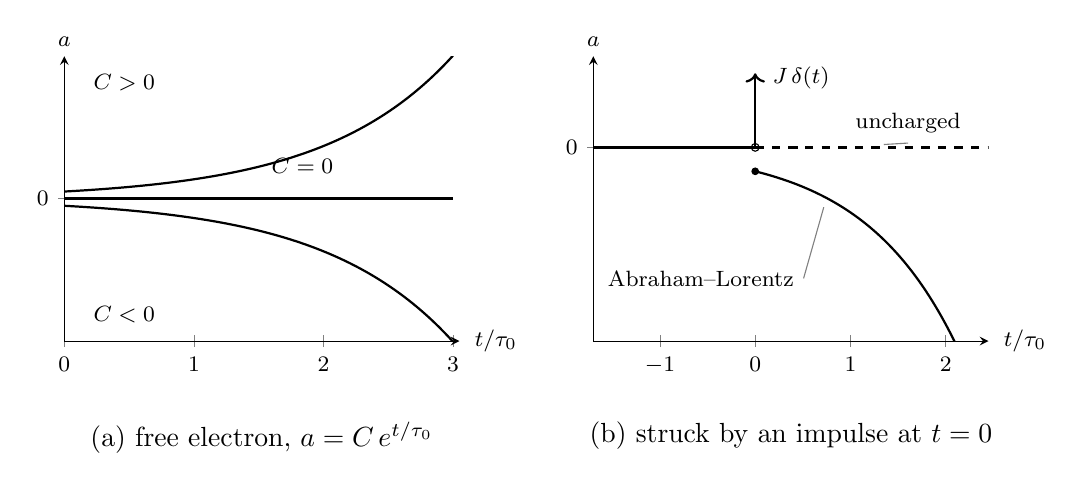
\begin{tikzpicture}

%% ---------------- panel (a): the free electron ----------------
\begin{axis}[
  name=free,
  width=6.6cm, height=5.2cm,
  xlabel={$t/\tau_0$}, ylabel={$a$},
  xmin=0, xmax=3.05, ymin=-3.2, ymax=3.2,
  axis lines=left,
  ytick={0}, yticklabels={$0$},
  xtick={0,1,2,3},
  every axis y label/.style={at={(ticklabel* cs:1.0)},anchor=south},
  every axis x label/.style={at={(ticklabel* cs:1.0)},anchor=west,
                             xshift=2pt},
  clip=true, samples=80, font=\footnotesize,
]
  \addplot[domain=0:3,thick] {0.16*exp(x)};
  \addplot[domain=0:3,thick] {-0.16*exp(x)};
  \addplot[domain=0:3,very thick] {0};
  \node[anchor=west,font=\footnotesize] at (axis cs:0.15,2.6)  {$C>0$};
  \node[anchor=west,font=\footnotesize] at (axis cs:0.15,-2.6) {$C<0$};
  \node[anchor=south east,font=\footnotesize] at (axis cs:2.15,0.35) {$C=0$};
\end{axis}
\node[anchor=north,align=center] at ([yshift=-9mm]free.south)
     {(a) free electron, $a=C\,e^{t/\tau_0}$};

%% ---------------- panel (b): struck by an impulse ----------------
\begin{axis}[
  name=imp,
  at={(free.east)}, anchor=west, xshift=1.7cm,
  width=6.6cm, height=5.2cm,
  xlabel={$t/\tau_0$}, ylabel={$a$},
  xmin=-1.7, xmax=2.45, ymin=-3.4, ymax=1.6,
  axis lines=left,
  ytick={0}, yticklabels={$0$},
  xtick={-1,0,1,2},
  every axis y label/.style={at={(ticklabel* cs:1.0)},anchor=south},
  every axis x label/.style={at={(ticklabel* cs:1.0)},anchor=west,
                             xshift=2pt},
  clip=true, samples=80, font=\footnotesize,
]
  %% before the blow: at rest
  \addplot[domain=-1.7:0,very thick] {0};
  %% uncharged particle: back to zero immediately
  \addplot[domain=0:2.45,very thick,dashed] {0};
  %% the impulse itself
  \draw[->,thick] (axis cs:0,0) -- (axis cs:0,1.3);
  \node[anchor=west,font=\footnotesize] at (axis cs:0.08,1.22) {$J\,\delta(t)$};
  %% Abraham-Lorentz: jumps the wrong way, then runs
  \addplot[domain=0:2.45,thick] {-0.42*exp(x)};
  \fill (axis cs:0,-0.42) circle (1.4pt);
  \draw (axis cs:0,0) circle (1.4pt);
  %% labels placed in the empty regions, with leaders
  \node[anchor=west,font=\footnotesize] (unch) at (axis cs:0.95,0.42)
       {uncharged};
  \draw[gray] (unch.south) -- (axis cs:1.35,0.05);
  \node[anchor=west,font=\footnotesize] (al) at (axis cs:-1.65,-2.3)
       {Abraham--Lorentz};
  \draw[gray] (al.east) -- (axis cs:0.72,-1.05);
\end{axis}
\node[anchor=north,align=center] at ([yshift=-9mm]imp.south)
     {(b) struck by an impulse at $t=0$};

\end{tikzpicture}
\caption{The two faces of the third-order term. \emph{(a)} A free electron
obeying Eq.~(\ref{eq:AL}) has $a = C\,e^{t/\tau_0}$. Every $C\ne0$ runs away;
the physical solution is the single value $C=0$, and nothing in the
initial-value problem selects it, since the equation is first order in $a$ and
admits any $a(0)$. \emph{(b)} An impulse delivered at $t=0$. An uncharged
particle takes the blow, jumps in velocity, and returns to zero acceleration:
the force is over and so is the acceleration. The electron does the opposite.
Its acceleration jumps to $\kappa = -J/m\tau_0$ and grows without bound long
after nothing is acting on it, and, since $\kappa$ carries the sign opposite to
$J$, it runs away against the blow that started it. The velocity, by contrast,
is continuous at $t=0$ here: it is the acceleration that jumps.
\label{fig:runaway}}
\end{figure}
.
%% Needs pgfplots, loaded in the main preamble.
%%
%% Panel (a) plots a = C exp(t/tau_0) for three values of C. Panel (b) plots
%% the impulse response of Eq. (AL): a = 0 before the blow and
%% a = kappa exp(t/tau_0) after it, with kappa = -J/(m tau_0). The sign is the
%% point of the panel and is not a drawing choice -- integrating
%% m a - m tau_0 adot = J delta(t) across t = 0 gives a jump of -J/(m tau_0),
%% so the runaway is directed against the impulse.

\begin{figure}[htb]
\centering
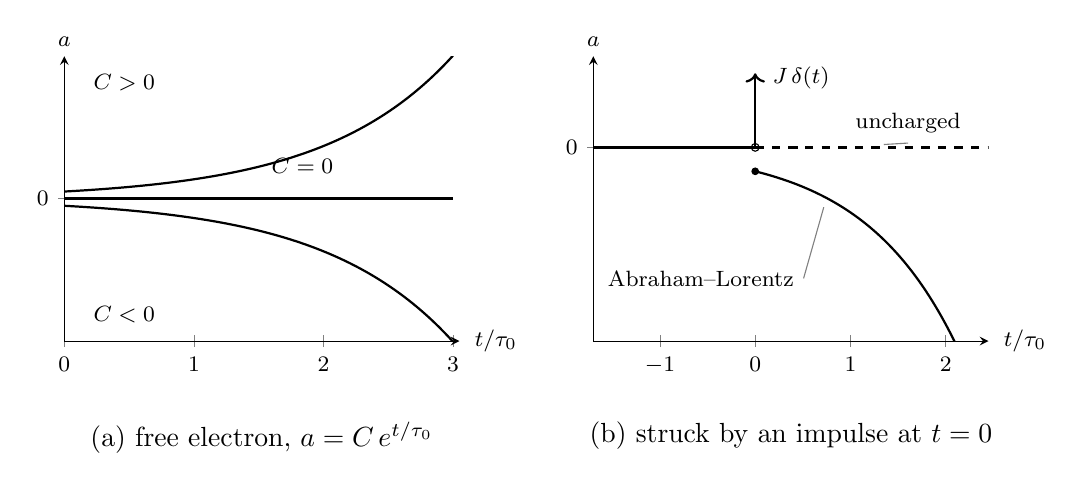
\begin{tikzpicture}

%% ---------------- panel (a): the free electron ----------------
\begin{axis}[
  name=free,
  width=6.6cm, height=5.2cm,
  xlabel={$t/\tau_0$}, ylabel={$a$},
  xmin=0, xmax=3.05, ymin=-3.2, ymax=3.2,
  axis lines=left,
  ytick={0}, yticklabels={$0$},
  xtick={0,1,2,3},
  every axis y label/.style={at={(ticklabel* cs:1.0)},anchor=south},
  every axis x label/.style={at={(ticklabel* cs:1.0)},anchor=west,
                             xshift=2pt},
  clip=true, samples=80, font=\footnotesize,
]
  \addplot[domain=0:3,thick] {0.16*exp(x)};
  \addplot[domain=0:3,thick] {-0.16*exp(x)};
  \addplot[domain=0:3,very thick] {0};
  \node[anchor=west,font=\footnotesize] at (axis cs:0.15,2.6)  {$C>0$};
  \node[anchor=west,font=\footnotesize] at (axis cs:0.15,-2.6) {$C<0$};
  \node[anchor=south east,font=\footnotesize] at (axis cs:2.15,0.35) {$C=0$};
\end{axis}
\node[anchor=north,align=center] at ([yshift=-9mm]free.south)
     {(a) free electron, $a=C\,e^{t/\tau_0}$};

%% ---------------- panel (b): struck by an impulse ----------------
\begin{axis}[
  name=imp,
  at={(free.east)}, anchor=west, xshift=1.7cm,
  width=6.6cm, height=5.2cm,
  xlabel={$t/\tau_0$}, ylabel={$a$},
  xmin=-1.7, xmax=2.45, ymin=-3.4, ymax=1.6,
  axis lines=left,
  ytick={0}, yticklabels={$0$},
  xtick={-1,0,1,2},
  every axis y label/.style={at={(ticklabel* cs:1.0)},anchor=south},
  every axis x label/.style={at={(ticklabel* cs:1.0)},anchor=west,
                             xshift=2pt},
  clip=true, samples=80, font=\footnotesize,
]
  %% before the blow: at rest
  \addplot[domain=-1.7:0,very thick] {0};
  %% uncharged particle: back to zero immediately
  \addplot[domain=0:2.45,very thick,dashed] {0};
  %% the impulse itself
  \draw[->,thick] (axis cs:0,0) -- (axis cs:0,1.3);
  \node[anchor=west,font=\footnotesize] at (axis cs:0.08,1.22) {$J\,\delta(t)$};
  %% Abraham-Lorentz: jumps the wrong way, then runs
  \addplot[domain=0:2.45,thick] {-0.42*exp(x)};
  \fill (axis cs:0,-0.42) circle (1.4pt);
  \draw (axis cs:0,0) circle (1.4pt);
  %% labels placed in the empty regions, with leaders
  \node[anchor=west,font=\footnotesize] (unch) at (axis cs:0.95,0.42)
       {uncharged};
  \draw[gray] (unch.south) -- (axis cs:1.35,0.05);
  \node[anchor=west,font=\footnotesize] (al) at (axis cs:-1.65,-2.3)
       {Abraham--Lorentz};
  \draw[gray] (al.east) -- (axis cs:0.72,-1.05);
\end{axis}
\node[anchor=north,align=center] at ([yshift=-9mm]imp.south)
     {(b) struck by an impulse at $t=0$};

\end{tikzpicture}
\caption{The two faces of the third-order term. \emph{(a)} A free electron
obeying Eq.~(\ref{eq:AL}) has $a = C\,e^{t/\tau_0}$. Every $C\ne0$ runs away;
the physical solution is the single value $C=0$, and nothing in the
initial-value problem selects it, since the equation is first order in $a$ and
admits any $a(0)$. \emph{(b)} An impulse delivered at $t=0$. An uncharged
particle takes the blow, jumps in velocity, and returns to zero acceleration:
the force is over and so is the acceleration. The electron does the opposite.
Its acceleration jumps to $\kappa = -J/m\tau_0$ and grows without bound long
after nothing is acting on it, and, since $\kappa$ carries the sign opposite to
$J$, it runs away against the blow that started it. The velocity, by contrast,
is continuous at $t=0$ here: it is the acceleration that jumps.
\label{fig:runaway}}
\end{figure}
.
%% Needs pgfplots, loaded in the main preamble.
%%
%% Panel (a) plots a = C exp(t/tau_0) for three values of C. Panel (b) plots
%% the impulse response of Eq. (AL): a = 0 before the blow and
%% a = kappa exp(t/tau_0) after it, with kappa = -J/(m tau_0). The sign is the
%% point of the panel and is not a drawing choice -- integrating
%% m a - m tau_0 adot = J delta(t) across t = 0 gives a jump of -J/(m tau_0),
%% so the runaway is directed against the impulse.

\begin{figure}[htb]
\centering
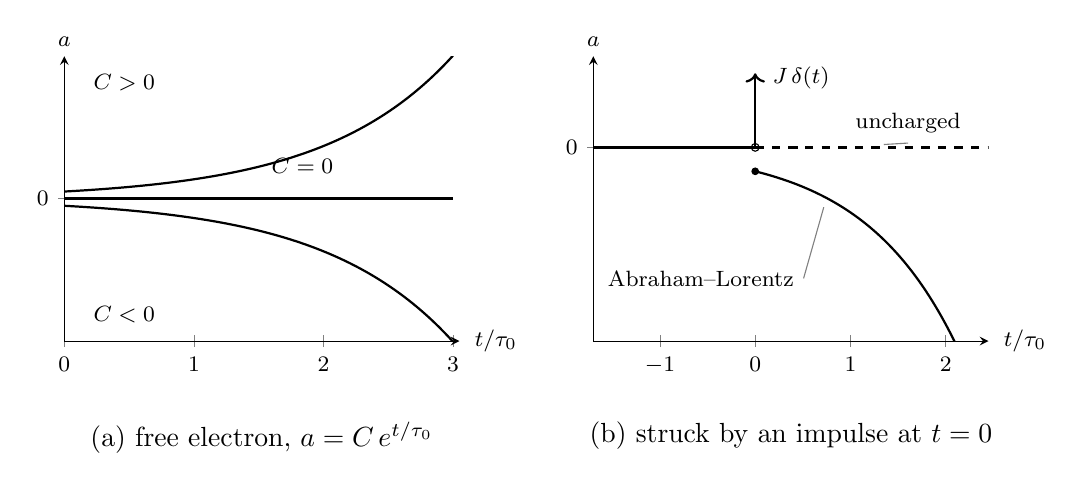
\begin{tikzpicture}

%% ---------------- panel (a): the free electron ----------------
\begin{axis}[
  name=free,
  width=6.6cm, height=5.2cm,
  xlabel={$t/\tau_0$}, ylabel={$a$},
  xmin=0, xmax=3.05, ymin=-3.2, ymax=3.2,
  axis lines=left,
  ytick={0}, yticklabels={$0$},
  xtick={0,1,2,3},
  every axis y label/.style={at={(ticklabel* cs:1.0)},anchor=south},
  every axis x label/.style={at={(ticklabel* cs:1.0)},anchor=west,
                             xshift=2pt},
  clip=true, samples=80, font=\footnotesize,
]
  \addplot[domain=0:3,thick] {0.16*exp(x)};
  \addplot[domain=0:3,thick] {-0.16*exp(x)};
  \addplot[domain=0:3,very thick] {0};
  \node[anchor=west,font=\footnotesize] at (axis cs:0.15,2.6)  {$C>0$};
  \node[anchor=west,font=\footnotesize] at (axis cs:0.15,-2.6) {$C<0$};
  \node[anchor=south east,font=\footnotesize] at (axis cs:2.15,0.35) {$C=0$};
\end{axis}
\node[anchor=north,align=center] at ([yshift=-9mm]free.south)
     {(a) free electron, $a=C\,e^{t/\tau_0}$};

%% ---------------- panel (b): struck by an impulse ----------------
\begin{axis}[
  name=imp,
  at={(free.east)}, anchor=west, xshift=1.7cm,
  width=6.6cm, height=5.2cm,
  xlabel={$t/\tau_0$}, ylabel={$a$},
  xmin=-1.7, xmax=2.45, ymin=-3.4, ymax=1.6,
  axis lines=left,
  ytick={0}, yticklabels={$0$},
  xtick={-1,0,1,2},
  every axis y label/.style={at={(ticklabel* cs:1.0)},anchor=south},
  every axis x label/.style={at={(ticklabel* cs:1.0)},anchor=west,
                             xshift=2pt},
  clip=true, samples=80, font=\footnotesize,
]
  %% before the blow: at rest
  \addplot[domain=-1.7:0,very thick] {0};
  %% uncharged particle: back to zero immediately
  \addplot[domain=0:2.45,very thick,dashed] {0};
  %% the impulse itself
  \draw[->,thick] (axis cs:0,0) -- (axis cs:0,1.3);
  \node[anchor=west,font=\footnotesize] at (axis cs:0.08,1.22) {$J\,\delta(t)$};
  %% Abraham-Lorentz: jumps the wrong way, then runs
  \addplot[domain=0:2.45,thick] {-0.42*exp(x)};
  \fill (axis cs:0,-0.42) circle (1.4pt);
  \draw (axis cs:0,0) circle (1.4pt);
  %% labels placed in the empty regions, with leaders
  \node[anchor=west,font=\footnotesize] (unch) at (axis cs:0.95,0.42)
       {uncharged};
  \draw[gray] (unch.south) -- (axis cs:1.35,0.05);
  \node[anchor=west,font=\footnotesize] (al) at (axis cs:-1.65,-2.3)
       {Abraham--Lorentz};
  \draw[gray] (al.east) -- (axis cs:0.72,-1.05);
\end{axis}
\node[anchor=north,align=center] at ([yshift=-9mm]imp.south)
     {(b) struck by an impulse at $t=0$};

\end{tikzpicture}
\caption{The two faces of the third-order term. \emph{(a)} A free electron
obeying Eq.~(\ref{eq:AL}) has $a = C\,e^{t/\tau_0}$. Every $C\ne0$ runs away;
the physical solution is the single value $C=0$, and nothing in the
initial-value problem selects it, since the equation is first order in $a$ and
admits any $a(0)$. \emph{(b)} An impulse delivered at $t=0$. An uncharged
particle takes the blow, jumps in velocity, and returns to zero acceleration:
the force is over and so is the acceleration. The electron does the opposite.
Its acceleration jumps to $\kappa = -J/m\tau_0$ and grows without bound long
after nothing is acting on it, and, since $\kappa$ carries the sign opposite to
$J$, it runs away against the blow that started it. The velocity, by contrast,
is continuous at $t=0$ here: it is the acceleration that jumps.
\label{fig:runaway}}
\end{figure}


Set $\mathbf F = 0$ in Eq.~(\ref{eq:AL}), keep only the two terms written, and
reduce to one dimension. The coefficient of the self-force term is $m$ times a
time,
\begin{equation}
\taunought = \frac{2e^2}{3mc^3} = 6.27\times10^{-24}~{\rm s}
\quad(\text{electron}),
\label{eq:tau0}
\end{equation}
which will reappear in every section below, and the equation of motion of a free
electron collapses to a first-order equation for the acceleration alone,
\begin{equation}
\dot a = \frac{a}{\taunought},
\qquad\text{whence}\qquad
a = C\,e^{\,t/\taunought}.
\label{eq:runawaysol}
\end{equation}

Both branches of this solution are unsatisfactory, and for different reasons.
If $C \neq 0$, an electron with nothing whatever acting on it accelerates
itself, and does so on the timescale $\taunought$, which is to say it gains a
factor of $e$ in acceleration every ${\sim}10^{-23}$ seconds. In the nonrelativistic
equation the velocity grows without bound. In the covariant version of
Sec.~\ref{sec:LDdisc} it approaches $c$ instead, but the character of the
solution is unchanged. No intuition about free particles survives this, and no
agent is available to be held responsible for the energy.

If $C = 0$ then $a = 0$, the electron moves uniformly, and Newton's first law is
recovered. One may say that the Abraham--Lorentz equation tells us that a free
electron moves exactly as an uncharged body does. The physical content is
unobjectionable. What is objectionable is the standing of the condition.
Equation~(\ref{eq:runawaysol}) is first order in $a$ and therefore admits any
initial value $a(0)$. The physical solution is picked out by setting $a(0)=0$,
and the only reason offered for doing so is that every other choice misbehaves
as $t\to\infty$. A condition imposed at infinity to restrict data at $t=0$ has
no warrant in the initial-value problem it is being applied to. This remains
true no matter how reasonable the surviving solution looks.

The impulse problem sharpens the objection into something concrete. Write the
electron's equation with an impulsive force of strength $J$ delivered at $t=0$,
\begin{equation}
ma - m\taunought\,\dot a = J\,\delta(t),
\label{eq:impulse}
\end{equation}
and compare with the corresponding classical problem. A free mass point struck
by an impulse jumps discontinuously in velocity and has zero acceleration
immediately afterwards: the blow is over, and so is the acceleration. Solving
Eq.~(\ref{eq:impulse}) with the electron moving uniformly beforehand gives
instead
\begin{equation}
a =
\begin{cases}
0, & t<0,\\[2pt]
\kappa\, e^{\,t/\taunought}, & t>0,
\end{cases}
\qquad \kappa = -\frac{J}{m\taunought}.
\label{eq:impulsesol}
\end{equation}
The electron does not stop accelerating when the blow ends. It accelerates ever
harder, without limit, long after nothing is acting on it. Since $\kappa$
carries the opposite sign to $J$, it runs away in the direction opposite to the
blow that started it. This is the runaway, or acceleration collapse, in its
starkest form. No choice of initial data avoids it here, because the requirement
of uniform motion before the pulse has already been spent.

The root of the behaviour is visible in the order of the equation. Newton's
equation of motion contains the acceleration and nothing beyond it, so when the
force stops the acceleration stops with it. Equation~(\ref{eq:AL}) contains
derivatives of the acceleration, so the state of the electron at a given instant
includes how fast its acceleration is changing, and that quantity survives the
force that produced it. What sustains it, physically, is the electron's own
electromagnetic field. The defect is therefore not an artefact of the sphere
model or of the expansion used to reach Eq.~(\ref{eq:AL}). Any equation of
motion that accounts for the self-field by adding a derivative of the
acceleration will inherit it. Dirac's equation, derived on entirely different
principles in Sec.~\ref{sec:LDderiv}, inherits it exactly.

\subsection{Criteria for a physically acceptable equation of motion}
\label{sec:criteria}

Everything from here on consists of proposals to replace Eq.~(\ref{eq:AL}) with
something better behaved, and proposals cannot be judged without a standard to
judge them by. It is worth fixing that standard now, before any candidate is on
the table, so that it cannot be quietly adjusted to fit whichever equation is
under discussion. Three requirements are imposed throughout these notes.

\begin{enumerate}

\item \textbf{The motion must follow from the equation in the ordinary way.}
\label{crit:ivp}
The particle should obey a differential equation that can be solved by the usual
procedure. One supplies initial or boundary data, integrates, and obtains the
state at all later times. The data supplied must themselves be data the physical
situation could actually provide. This is a weaker demand than it may appear,
and Sec.~\ref{sec:runaway} has already shown Eq.~(\ref{eq:AL}) failing it: the
equation is solvable, but the solution that survives is picked out by a
condition imposed at $t\to\infty$, and no experimenter preparing an electron at
$t=0$ has access to that condition.

\item \textbf{A stable state must remain stable under a small disturbance.}
\label{crit:stability}
The concrete test used throughout is the one already applied in
Sec.~\ref{sec:runaway}: take a particle in uniform motion, strike it with a
pulse, and ask what it does afterwards. An acceptable equation returns it to
uniform motion. It is also acceptable for the particle to settle into a regular
variation confined to a bounded range of speeds. This weaker alternative is
included deliberately, because Sec.~\ref{sec:eliezer} produces solutions of
exactly this kind. What is not acceptable is for the
particle to accelerate without limit toward $c$, or to swing back and forth
between $+c$ and $-c$. Both are read here as signs that the equation has no
stable state to return to, rather than as physics.

\item \textbf{The ordinary physical laws must hold.}
\label{crit:conservation}
Energy conservation and causality are not negotiable, and an equation that
purchases good behaviour by breaking either has not solved the problem but
relocated it. This criterion does the least work in the pages that follow and is
the easiest to forget, which is why it is worth writing down. The sign of a
radiation-reaction term, for instance, is exactly the kind of thing one may
change to remove a runaway without noticing what it does to the energy budget.

\end{enumerate}

These three are the scorecard. Sections~\ref{sec:LDdisc}, \ref{sec:lk} and
\ref{sec:eliezer} each close by returning to them. Two features of the list are
worth noticing before it is used. It is stated entirely in terms of the
behaviour of solutions and says nothing about the form an equation should take,
which is deliberate, since the strategy of the sections that follow is precisely
to alter the form and inspect what comes out. And it asks that a charged
particle behave, in these respects, like an ordinary mechanical one. That
expectation is reasonable and widely shared, but it is worth flagging as an
assumption rather than a deduction.

%% ===================================================================
\section{The Lorentz--Dirac Equation: Derivation}
\label{sec:LDderiv}

A word on the name before the derivation. Throughout these notes
\emph{Lorentz--Dirac}, abbreviated LD and also found in the literature as
Abraham--Lorentz--Dirac, means the classical equation of motion of a point
charge derived below and tagged (LD). It never means Dirac's relativistic wave
equation, with which it has nothing in common but its author.

\subsection{The world-tube momentum--energy balance}
\label{sec:tube}

%% figures/fig-tube.tex -- Figure 1, Dirac's world tube.
%% Pulled into notes.tex with %% figures/fig-tube.tex -- Figure 1, Dirac's world tube.
%% Pulled into notes.tex with %% figures/fig-tube.tex -- Figure 1, Dirac's world tube.
%% Pulled into notes.tex with \input{figures/fig-tube}.
%% Needs tikz with the arrows.meta library, loaded in the main preamble.
%%
%% Geometry note: the world line is x = 0.3*sin(45 s), so dx/ds vanishes
%% at s = 2. The point annotated in panel (a) is placed there, which is
%% why u(tau) can be drawn straight up and the separation exactly
%% horizontal -- the right angle in the figure is true, not suggested.

\begin{figure}[htb]
\centering
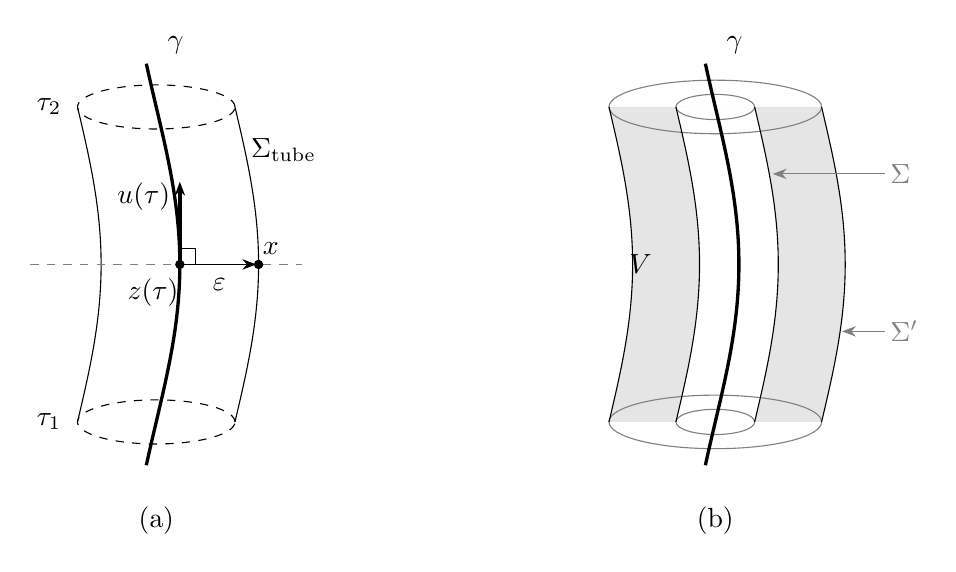
\begin{tikzpicture}[>={Stealth[length=5pt]},line join=round]

%% ---------------- panel (a): the tube construction ----------------
\begin{scope}
  %% end caps, dashed: the integration is over the wall only
  \draw[dashed] (0,0) ellipse [x radius=1, y radius=0.28];
  \draw[dashed] (0,4) ellipse [x radius=1, y radius=0.28];
  %% tube walls
  \draw plot[domain=0:4,samples=80,smooth] ({0.3*sin(45*\x) - 1},\x);
  \draw plot[domain=0:4,samples=80,smooth] ({0.3*sin(45*\x) + 1},\x);
  %% hyperplane of simultaneity through z(tau)
  \draw[dashed,gray] (-1.6,2) -- (1.85,2);
  %% world line, drawn through both caps so it reads as a line
  \draw[very thick] plot[domain=-0.55:4.55,samples=90,smooth]
       ({0.3*sin(45*\x)},\x);
  \node[right] at (0.02,4.78) {$\gamma$};
  %% proper times
  \node[left] at (-1.08,0) {$\tau_1$};
  \node[left] at (-1.08,4) {$\tau_2$};
  %% annotated point: world line is momentarily vertical here, so u is
  %% straight up and the separation is horizontal
  \draw[->,very thick] (0.3,2) -- (0.3,3.05);
  \node[left] at (0.3,2.86) {$u(\tau)$};
  \draw[->] (0.3,2) -- (1.27,2);
  \node[below] at (0.8,1.95) {$\varepsilon$};
  \draw (0.3,2.2) -- (0.5,2.2) -- (0.5,2);
  \fill (0.3,2) circle (1.7pt);
  \node[below left,xshift=3pt] at (0.3,1.94) {$z(\tau)$};
  \fill (1.3,2) circle (1.7pt);
  \node[above right,xshift=-2pt] at (1.3,2.0) {$x$};
  \node[right] at (1.08,3.45) {$\Sigma_{\rm tube}$};
  \node at (0,-1.25) {(a)};
\end{scope}

%% ---------------- panel (b): the choice of tube is immaterial ----------
\begin{scope}[xshift=7.1cm]
  %% source-free region between the two tubes
  \fill[gray!20]
     plot[domain=0:4,samples=80,smooth] ({0.3*sin(45*\x) - 1.35},\x)
  -- plot[domain=4:0,samples=80,smooth] ({0.3*sin(45*\x) + 1.35},\x)
  -- cycle;
  \fill[white]
     plot[domain=0:4,samples=80,smooth] ({0.3*sin(45*\x) - 0.5},\x)
  -- plot[domain=4:0,samples=80,smooth] ({0.3*sin(45*\x) + 0.5},\x)
  -- cycle;
  %% caps, so both surfaces read as tubes
  \draw[gray] (0,0) ellipse [x radius=1.35, y radius=0.34];
  \draw[gray] (0,4) ellipse [x radius=1.35, y radius=0.34];
  \draw[gray] (0,0) ellipse [x radius=0.5,  y radius=0.16];
  \draw[gray] (0,4) ellipse [x radius=0.5,  y radius=0.16];
  %% walls
  \draw plot[domain=0:4,samples=80,smooth] ({0.3*sin(45*\x) - 0.5},\x);
  \draw plot[domain=0:4,samples=80,smooth] ({0.3*sin(45*\x) + 0.5},\x);
  \draw plot[domain=0:4,samples=80,smooth] ({0.3*sin(45*\x) - 1.35},\x);
  \draw plot[domain=0:4,samples=80,smooth] ({0.3*sin(45*\x) + 1.35},\x);
  \draw[very thick] plot[domain=-0.55:4.55,samples=90,smooth]
       ({0.3*sin(45*\x)},\x);
  \node[right] at (0.02,4.78) {$\gamma$};
  %% leaders to the two walls
  \draw[->,gray] (2.15,3.15) -- (0.73,3.15);
  \node[right,gray] at (2.1,3.15) {$\Sigma$};
  \draw[->,gray] (2.15,1.15) -- (1.61,1.15);
  \node[right,gray] at (2.1,1.15) {$\Sigma'$};
  \node at (-0.95,2) {$V$};
  \node at (0,-1.25) {(b)};
\end{scope}

\end{tikzpicture}
\caption{Dirac's construction. \emph{(a)} The tube. At each proper time the
point $z(\tau)$ on the world line $\gamma$ carries a sphere of radius
$\varepsilon$, drawn in the hyperplane of simultaneity of $z(\tau)$ --- the
dashed line --- so that the separation $x-z(\tau)$ to a point $x$ of the tube is
orthogonal to the four-velocity $u(\tau)$, as in Eq.~(\ref{eq:diractube}).
Dragging that sphere along $\gamma$ from $\tau_1$ to $\tau_2$ sweeps out
$\Sigma_{\rm tube}$. The end caps are drawn dashed as a reminder that the
integration is carried out over the wall alone; see
Sec.~\ref{sec:reservations}. \emph{(b)} Why the choice of tube does not matter.
Two tubes $\Sigma$ and $\Sigma'$ enclose the same world line, and the region
$V$ between them contains no charge, so the flux of $T^{\mu\nu}$ through the two
is the same by Eq.~(\ref{eq:tubeindep}). The balance may therefore be read on
any surface, including one that keeps well away from the singular world line.
\label{fig:tube}}
\end{figure}
.
%% Needs tikz with the arrows.meta library, loaded in the main preamble.
%%
%% Geometry note: the world line is x = 0.3*sin(45 s), so dx/ds vanishes
%% at s = 2. The point annotated in panel (a) is placed there, which is
%% why u(tau) can be drawn straight up and the separation exactly
%% horizontal -- the right angle in the figure is true, not suggested.

\begin{figure}[htb]
\centering
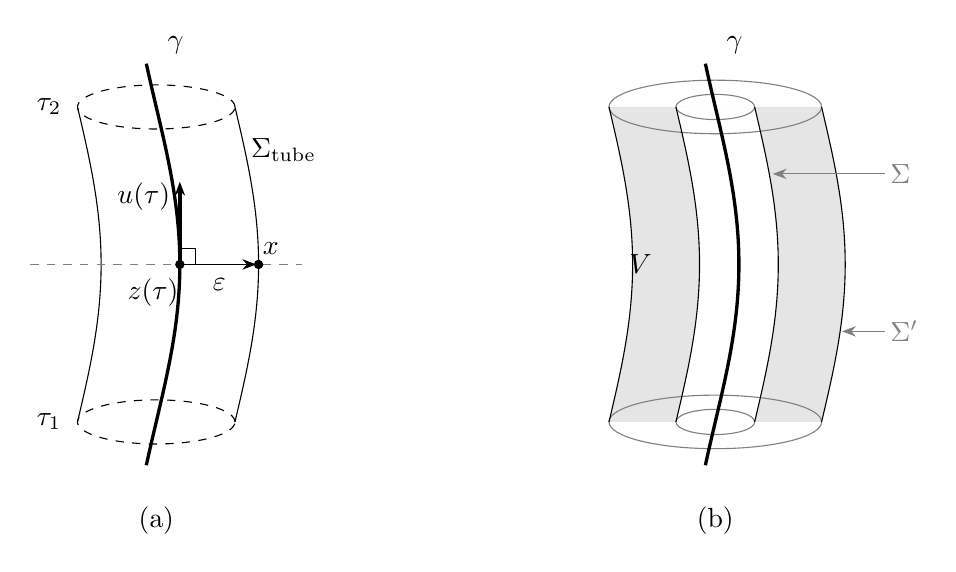
\begin{tikzpicture}[>={Stealth[length=5pt]},line join=round]

%% ---------------- panel (a): the tube construction ----------------
\begin{scope}
  %% end caps, dashed: the integration is over the wall only
  \draw[dashed] (0,0) ellipse [x radius=1, y radius=0.28];
  \draw[dashed] (0,4) ellipse [x radius=1, y radius=0.28];
  %% tube walls
  \draw plot[domain=0:4,samples=80,smooth] ({0.3*sin(45*\x) - 1},\x);
  \draw plot[domain=0:4,samples=80,smooth] ({0.3*sin(45*\x) + 1},\x);
  %% hyperplane of simultaneity through z(tau)
  \draw[dashed,gray] (-1.6,2) -- (1.85,2);
  %% world line, drawn through both caps so it reads as a line
  \draw[very thick] plot[domain=-0.55:4.55,samples=90,smooth]
       ({0.3*sin(45*\x)},\x);
  \node[right] at (0.02,4.78) {$\gamma$};
  %% proper times
  \node[left] at (-1.08,0) {$\tau_1$};
  \node[left] at (-1.08,4) {$\tau_2$};
  %% annotated point: world line is momentarily vertical here, so u is
  %% straight up and the separation is horizontal
  \draw[->,very thick] (0.3,2) -- (0.3,3.05);
  \node[left] at (0.3,2.86) {$u(\tau)$};
  \draw[->] (0.3,2) -- (1.27,2);
  \node[below] at (0.8,1.95) {$\varepsilon$};
  \draw (0.3,2.2) -- (0.5,2.2) -- (0.5,2);
  \fill (0.3,2) circle (1.7pt);
  \node[below left,xshift=3pt] at (0.3,1.94) {$z(\tau)$};
  \fill (1.3,2) circle (1.7pt);
  \node[above right,xshift=-2pt] at (1.3,2.0) {$x$};
  \node[right] at (1.08,3.45) {$\Sigma_{\rm tube}$};
  \node at (0,-1.25) {(a)};
\end{scope}

%% ---------------- panel (b): the choice of tube is immaterial ----------
\begin{scope}[xshift=7.1cm]
  %% source-free region between the two tubes
  \fill[gray!20]
     plot[domain=0:4,samples=80,smooth] ({0.3*sin(45*\x) - 1.35},\x)
  -- plot[domain=4:0,samples=80,smooth] ({0.3*sin(45*\x) + 1.35},\x)
  -- cycle;
  \fill[white]
     plot[domain=0:4,samples=80,smooth] ({0.3*sin(45*\x) - 0.5},\x)
  -- plot[domain=4:0,samples=80,smooth] ({0.3*sin(45*\x) + 0.5},\x)
  -- cycle;
  %% caps, so both surfaces read as tubes
  \draw[gray] (0,0) ellipse [x radius=1.35, y radius=0.34];
  \draw[gray] (0,4) ellipse [x radius=1.35, y radius=0.34];
  \draw[gray] (0,0) ellipse [x radius=0.5,  y radius=0.16];
  \draw[gray] (0,4) ellipse [x radius=0.5,  y radius=0.16];
  %% walls
  \draw plot[domain=0:4,samples=80,smooth] ({0.3*sin(45*\x) - 0.5},\x);
  \draw plot[domain=0:4,samples=80,smooth] ({0.3*sin(45*\x) + 0.5},\x);
  \draw plot[domain=0:4,samples=80,smooth] ({0.3*sin(45*\x) - 1.35},\x);
  \draw plot[domain=0:4,samples=80,smooth] ({0.3*sin(45*\x) + 1.35},\x);
  \draw[very thick] plot[domain=-0.55:4.55,samples=90,smooth]
       ({0.3*sin(45*\x)},\x);
  \node[right] at (0.02,4.78) {$\gamma$};
  %% leaders to the two walls
  \draw[->,gray] (2.15,3.15) -- (0.73,3.15);
  \node[right,gray] at (2.1,3.15) {$\Sigma$};
  \draw[->,gray] (2.15,1.15) -- (1.61,1.15);
  \node[right,gray] at (2.1,1.15) {$\Sigma'$};
  \node at (-0.95,2) {$V$};
  \node at (0,-1.25) {(b)};
\end{scope}

\end{tikzpicture}
\caption{Dirac's construction. \emph{(a)} The tube. At each proper time the
point $z(\tau)$ on the world line $\gamma$ carries a sphere of radius
$\varepsilon$, drawn in the hyperplane of simultaneity of $z(\tau)$ --- the
dashed line --- so that the separation $x-z(\tau)$ to a point $x$ of the tube is
orthogonal to the four-velocity $u(\tau)$, as in Eq.~(\ref{eq:diractube}).
Dragging that sphere along $\gamma$ from $\tau_1$ to $\tau_2$ sweeps out
$\Sigma_{\rm tube}$. The end caps are drawn dashed as a reminder that the
integration is carried out over the wall alone; see
Sec.~\ref{sec:reservations}. \emph{(b)} Why the choice of tube does not matter.
Two tubes $\Sigma$ and $\Sigma'$ enclose the same world line, and the region
$V$ between them contains no charge, so the flux of $T^{\mu\nu}$ through the two
is the same by Eq.~(\ref{eq:tubeindep}). The balance may therefore be read on
any surface, including one that keeps well away from the singular world line.
\label{fig:tube}}
\end{figure}
.
%% Needs tikz with the arrows.meta library, loaded in the main preamble.
%%
%% Geometry note: the world line is x = 0.3*sin(45 s), so dx/ds vanishes
%% at s = 2. The point annotated in panel (a) is placed there, which is
%% why u(tau) can be drawn straight up and the separation exactly
%% horizontal -- the right angle in the figure is true, not suggested.

\begin{figure}[htb]
\centering
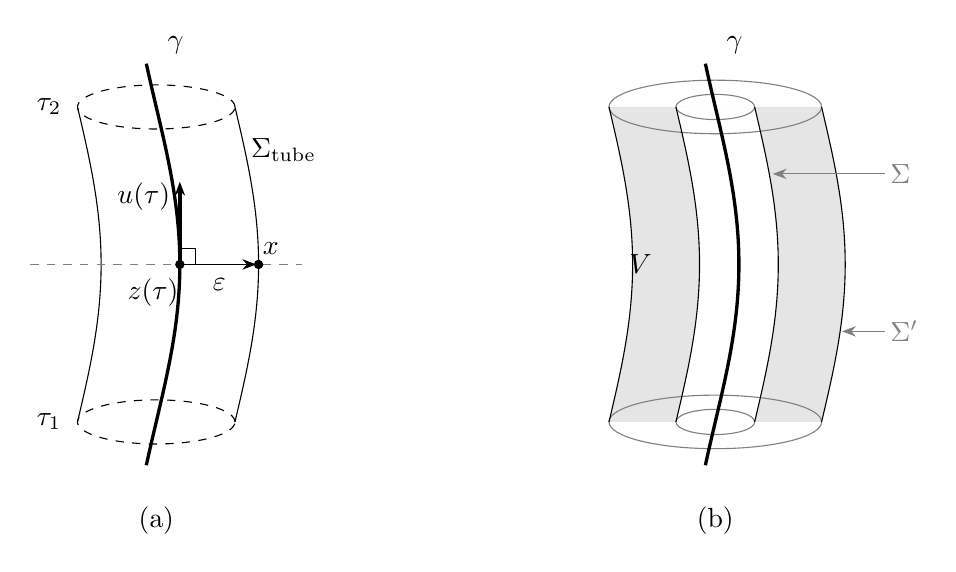
\begin{tikzpicture}[>={Stealth[length=5pt]},line join=round]

%% ---------------- panel (a): the tube construction ----------------
\begin{scope}
  %% end caps, dashed: the integration is over the wall only
  \draw[dashed] (0,0) ellipse [x radius=1, y radius=0.28];
  \draw[dashed] (0,4) ellipse [x radius=1, y radius=0.28];
  %% tube walls
  \draw plot[domain=0:4,samples=80,smooth] ({0.3*sin(45*\x) - 1},\x);
  \draw plot[domain=0:4,samples=80,smooth] ({0.3*sin(45*\x) + 1},\x);
  %% hyperplane of simultaneity through z(tau)
  \draw[dashed,gray] (-1.6,2) -- (1.85,2);
  %% world line, drawn through both caps so it reads as a line
  \draw[very thick] plot[domain=-0.55:4.55,samples=90,smooth]
       ({0.3*sin(45*\x)},\x);
  \node[right] at (0.02,4.78) {$\gamma$};
  %% proper times
  \node[left] at (-1.08,0) {$\tau_1$};
  \node[left] at (-1.08,4) {$\tau_2$};
  %% annotated point: world line is momentarily vertical here, so u is
  %% straight up and the separation is horizontal
  \draw[->,very thick] (0.3,2) -- (0.3,3.05);
  \node[left] at (0.3,2.86) {$u(\tau)$};
  \draw[->] (0.3,2) -- (1.27,2);
  \node[below] at (0.8,1.95) {$\varepsilon$};
  \draw (0.3,2.2) -- (0.5,2.2) -- (0.5,2);
  \fill (0.3,2) circle (1.7pt);
  \node[below left,xshift=3pt] at (0.3,1.94) {$z(\tau)$};
  \fill (1.3,2) circle (1.7pt);
  \node[above right,xshift=-2pt] at (1.3,2.0) {$x$};
  \node[right] at (1.08,3.45) {$\Sigma_{\rm tube}$};
  \node at (0,-1.25) {(a)};
\end{scope}

%% ---------------- panel (b): the choice of tube is immaterial ----------
\begin{scope}[xshift=7.1cm]
  %% source-free region between the two tubes
  \fill[gray!20]
     plot[domain=0:4,samples=80,smooth] ({0.3*sin(45*\x) - 1.35},\x)
  -- plot[domain=4:0,samples=80,smooth] ({0.3*sin(45*\x) + 1.35},\x)
  -- cycle;
  \fill[white]
     plot[domain=0:4,samples=80,smooth] ({0.3*sin(45*\x) - 0.5},\x)
  -- plot[domain=4:0,samples=80,smooth] ({0.3*sin(45*\x) + 0.5},\x)
  -- cycle;
  %% caps, so both surfaces read as tubes
  \draw[gray] (0,0) ellipse [x radius=1.35, y radius=0.34];
  \draw[gray] (0,4) ellipse [x radius=1.35, y radius=0.34];
  \draw[gray] (0,0) ellipse [x radius=0.5,  y radius=0.16];
  \draw[gray] (0,4) ellipse [x radius=0.5,  y radius=0.16];
  %% walls
  \draw plot[domain=0:4,samples=80,smooth] ({0.3*sin(45*\x) - 0.5},\x);
  \draw plot[domain=0:4,samples=80,smooth] ({0.3*sin(45*\x) + 0.5},\x);
  \draw plot[domain=0:4,samples=80,smooth] ({0.3*sin(45*\x) - 1.35},\x);
  \draw plot[domain=0:4,samples=80,smooth] ({0.3*sin(45*\x) + 1.35},\x);
  \draw[very thick] plot[domain=-0.55:4.55,samples=90,smooth]
       ({0.3*sin(45*\x)},\x);
  \node[right] at (0.02,4.78) {$\gamma$};
  %% leaders to the two walls
  \draw[->,gray] (2.15,3.15) -- (0.73,3.15);
  \node[right,gray] at (2.1,3.15) {$\Sigma$};
  \draw[->,gray] (2.15,1.15) -- (1.61,1.15);
  \node[right,gray] at (2.1,1.15) {$\Sigma'$};
  \node at (-0.95,2) {$V$};
  \node at (0,-1.25) {(b)};
\end{scope}

\end{tikzpicture}
\caption{Dirac's construction. \emph{(a)} The tube. At each proper time the
point $z(\tau)$ on the world line $\gamma$ carries a sphere of radius
$\varepsilon$, drawn in the hyperplane of simultaneity of $z(\tau)$ --- the
dashed line --- so that the separation $x-z(\tau)$ to a point $x$ of the tube is
orthogonal to the four-velocity $u(\tau)$, as in Eq.~(\ref{eq:diractube}).
Dragging that sphere along $\gamma$ from $\tau_1$ to $\tau_2$ sweeps out
$\Sigma_{\rm tube}$. The end caps are drawn dashed as a reminder that the
integration is carried out over the wall alone; see
Sec.~\ref{sec:reservations}. \emph{(b)} Why the choice of tube does not matter.
Two tubes $\Sigma$ and $\Sigma'$ enclose the same world line, and the region
$V$ between them contains no charge, so the flux of $T^{\mu\nu}$ through the two
is the same by Eq.~(\ref{eq:tubeindep}). The balance may therefore be read on
any surface, including one that keeps well away from the singular world line.
\label{fig:tube}}
\end{figure}


Dirac's advance was a change of question. Lorentz's route, followed in
Sec.~\ref{sec:lorentzmodel}, asks what force the charge exerts on itself and
answers by summing the retarded action of one charge element on another. That
sum has no meaning for a point charge, since the self-field diverges on the
world line. Dirac keeps the point charge and declines to ask about the force at
all. He asks instead where the energy and momentum go. Whatever the particle
radiates must be paid for out of the particle's own energy and momentum. That
balance can be struck without ever evaluating a field on the world line.
The divergent self-field still enters the calculation, but only through
differences, and the differences are finite.

\subsubsection{The tube, and why its shape is immaterial}
\label{sec:tubeindep}

Surround the world line $\gamma$ by a three-dimensional tube $\Sigma$. The
four-momentum crossing it is
\begin{equation}
\Delta P^\mu = \int_\Sigma T^{\mu\nu}\,d\Sigma_\nu .
\label{eq:tubeflux}
\end{equation}
Let $\Sigma$ and $\Sigma'$ both enclose $\gamma$, and let $V$ be the region
between them. That region contains no charge, so the stress--energy tensor is
conserved throughout it, and
\begin{equation}
\Delta P'^\mu - \Delta P^\mu
= \oint_{\partial V} T^{\mu\nu}\,d\Sigma_\nu
= \int_V T^{\mu\nu}{}_{,\nu}\,dV = 0 .
\label{eq:tubeindep}
\end{equation}

This is the whole reason the strategy beats Lorentz's. It deserves to be stated
on its own. A force must be evaluated somewhere, and for a point charge every
candidate location is a place where the field is infinite. A balance need not be
evaluated anywhere in particular. It may be read off on any surface at all,
including surfaces that keep a comfortable distance from the singularity.
Equation~(\ref{eq:tubeindep}) guarantees that the reading is the same. See
Fig.~\ref{fig:tube}(b).

Dirac's tube is the one adapted to the instantaneous rest frame. For a point $x$
on the tube, let $z(\tau)$ be the point of $\gamma$ satisfying
\begin{equation}
\left[x^\mu - z^\mu(\tau)\right]u_\mu(\tau) = 0 ,
\qquad
\left[x - z(\tau)\right]\cdot\left[x - z(\tau)\right] = \varepsilon^2 ,
\label{eq:diractube}
\end{equation}
the separation being spacelike. The first condition places $x$ on the hyperplane
of simultaneity of $z(\tau)$, so that ``at the same moment'' means at the same
moment for the particle. The second fixes the radius. Together they describe a
sphere of radius $\varepsilon$ drawn in the instantaneous rest frame and dragged
along the world line, sweeping out
$\Sigma_{\rm tube} = \{x(\tau,\varepsilon,\Omega);\ \tau_1\le\tau\le\tau_2\}$,
as in Fig.~\ref{fig:tube}(a).

\subsubsection{The surface element}
\label{sec:element}

Set $c=1$ for the rest of this subsection and work in the instantaneous rest
frame at proper time $\tau$, restoring $c$ at the end. Let $n^\mu$ be the unit
spacelike vector pointing from $z(\tau)$ to the point $x$ of the tube, so that
$x = z(\tau) + \varepsilon n$ with $n\cdot u = 0$ and $n\cdot n = 1$. Three
angular integrals are all that will be needed:
\begin{equation}
\oint d\Omega = 4\pi, \qquad
\oint n^i\,d\Omega = 0, \qquad
\oint n^i n^j\,d\Omega = \frac{4\pi}{3}\delta^{ij}.
\label{eq:angint}
\end{equation}

Differentiate $x = z + \varepsilon n$ along the world line at fixed $\Omega$.
The vector $n$ is Fermi--Walker transported, so
$\dot n^\mu = (a\cdot n)\,u^\mu$. Thus
\begin{equation}
\frac{\partial x^\mu}{\partial\tau} = u^\mu\left(1 + \varepsilon\,a\cdot n\right).
\label{eq:tubetilt}
\end{equation}
Each of the two angular directions contributes a factor $\varepsilon$. Thus
\begin{equation}
d\Sigma_\nu = n_\nu\,\varepsilon^2
\left(1 + \varepsilon\,a\cdot n\right) d\Omega\,d\tau .
\label{eq:tubeelement}
\end{equation}

The factor $1 + \varepsilon\,a\cdot n$ is the one thing in this subsection worth
memorizing. It is there because the tube is dragged along a world line that is
accelerating. Successive cross-sections are not parallel, and the wall stretches
on the side the particle is accelerating towards. It is also easy to write the
surface element without it, and everything that distinguishes this calculation
from the charged sphere of Sec.~\ref{sec:lorentzmodel} is contained in it.

\subsubsection{The field near the world line}
\label{sec:nearfield}

Expanded about $z(\tau)$ in the rest frame, the retarded field is
\begin{equation}
\mathbf E = \frac{e}{\varepsilon^2}\,\mathbf n
- \frac{e}{2\varepsilon}\left[\mathbf a + (\mathbf a\cdot\mathbf n)\mathbf n\right]
+ \frac{2e}{3}\,\dot{\mathbf a} + O(\varepsilon),
\label{eq:nearfield}
\end{equation}
while $\mathbf B$, which vanishes for a charge at rest, begins only at
$O(\varepsilon^{-1})$. The surface element carries $\varepsilon^2$, so a product
of two fields must reach $O(\varepsilon^{-3})$ to leave anything divergent
behind. Since $\mathbf{BB}$ is only $O(\varepsilon^{-2})$, the magnetic field
cannot contribute to the divergent term at all, and the whole of the next
subsubsection is an exercise with $\mathbf E$. The four-momentum leaving the
tube is
\begin{equation}
\frac{dP^\mu}{d\tau} = -\oint T^{\mu\nu} n_\nu\,
\varepsilon^2\left(1+\varepsilon\,a\cdot n\right)d\Omega ,
\qquad
T^{\mu\nu} = \frac{1}{4\pi}
\left[F^{\mu\alpha}F^{\nu}{}_{\alpha}
- \tfrac14\eta^{\mu\nu}F^{\alpha\beta}F_{\alpha\beta}\right].
\label{eq:fluxdef}
\end{equation}

\subsubsection{The divergent term, and what becomes of the $4/3$}
\label{sec:fourthirds}

%% figures/fig-simultaneity.tex -- Figure for Sec. 2.1.4.
%% Pulled into notes.tex with %% figures/fig-simultaneity.tex -- Figure for Sec. 2.1.4.
%% Pulled into notes.tex with %% figures/fig-simultaneity.tex -- Figure for Sec. 2.1.4.
%% Pulled into notes.tex with \input{figures/fig-simultaneity}.
%% Needs tikz with the arrows.meta library, loaded in the main preamble.
%%
%% Geometry: the world line is x = 0.18 t^2, so the velocity at time t is
%% v = 0.36 t. In an (x,t) diagram the simultaneity line of the instantaneous
%% rest frame at an event has slope dt/dx = v there, so the two slices drawn
%% in panel (a) have slopes 0.432 and 0.648 and cannot be parallel. Every
%% number below follows from those two lines; nothing is drawn by eye.

\begin{figure}[htb]
\centering
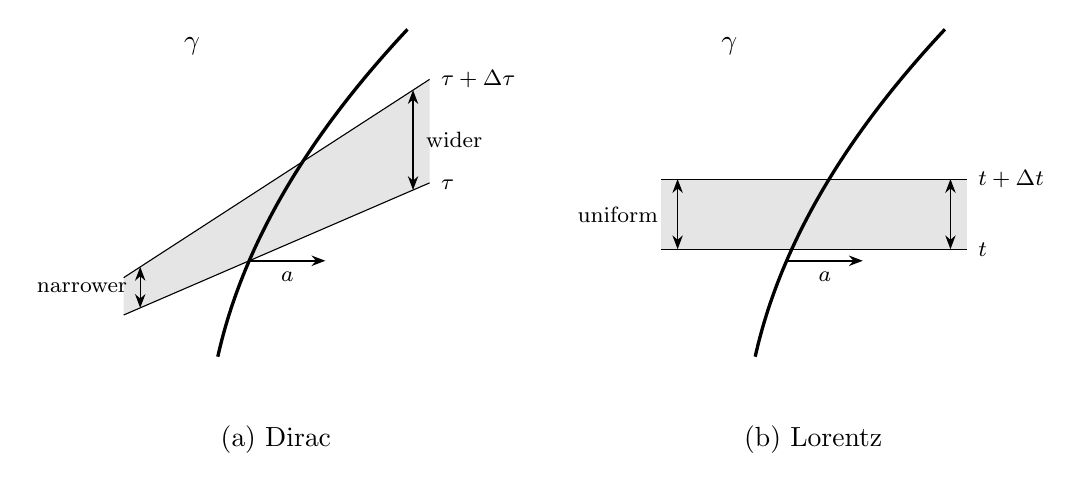
\begin{tikzpicture}[>={Stealth[length=5pt]},scale=2.1,line join=round]

%% ---------------- panel (a): the particle's own simultaneity ----------
\begin{scope}
  \fill[gray!20] (-0.5,0.872) -- (1.35,1.671) -- (1.35,2.297) -- (-0.5,1.098)
     -- cycle;
  %% the two rest-frame slices
  \draw (-0.5,0.872) -- (1.35,1.671);
  \draw (-0.5,1.098) -- (1.35,2.297);
  \node[right,font=\footnotesize] at (1.36,1.66) {$\tau$};
  \node[right,font=\footnotesize] at (1.36,2.30) {$\tau+\Delta\tau$};
  %% world line
  \draw[very thick] plot[domain=0.62:2.6,samples=60,smooth]
       ({0.18*\x*\x},\x);
  \node[left] at (0.02,2.5) {$\gamma$};
  %% acceleration
  \draw[->,thick] (0.259,1.2) -- (0.72,1.2);
  \node[below,font=\footnotesize] at (0.49,1.19) {$a$};
  %% the gap, measured at both ends
  \draw[<->] (-0.4,0.915) -- (-0.4,1.163);
  \draw[<->] (1.25,1.628) -- (1.25,2.232);
  \node[left,font=\footnotesize]  at (-0.42,1.04) {narrower};
  \node[right,font=\footnotesize] at (1.27,1.93) {wider};
  \node at (0.42,0.12) {(a) Dirac};
\end{scope}

%% ---------------- panel (b): constant time in one frame ---------------
\begin{scope}[xshift=3.25cm]
  \fill[gray!20] (-0.5,1.27) rectangle (1.35,1.694);
  \draw (-0.5,1.27)  -- (1.35,1.27);
  \draw (-0.5,1.694) -- (1.35,1.694);
  \node[right,font=\footnotesize] at (1.36,1.27)  {$t$};
  \node[right,font=\footnotesize] at (1.36,1.694) {$t+\Delta t$};
  \draw[very thick] plot[domain=0.62:2.6,samples=60,smooth]
       ({0.18*\x*\x},\x);
  \node[left] at (0.02,2.5) {$\gamma$};
  \draw[->,thick] (0.259,1.2) -- (0.72,1.2);
  \node[below,font=\footnotesize] at (0.49,1.19) {$a$};
  \draw[<->] (-0.4,1.27) -- (-0.4,1.694);
  \draw[<->] (1.25,1.27) -- (1.25,1.694);
  \node[left,font=\footnotesize]  at (-0.46,1.48) {uniform};
  \node at (0.42,0.12) {(b) Lorentz};
\end{scope}

\end{tikzpicture}
\caption{Where the $4/3$ goes. Both panels show the same accelerating world
line $\gamma$ and the same slab of it, and differ only in what is being called
``at the same moment''. \emph{(a)} Dirac's tube is built from the particle's own
succession of rest frames. Because the velocity changes along $\gamma$,
successive slices are not parallel: they fan open on the side the particle is
accelerating towards, and the slab is wider there. That fanning is the factor
$1+\varepsilon\,a\cdot n$ of Eq.~(\ref{eq:tubeelement}). \emph{(b)} Collecting
field momentum at constant time in one chosen frame gives parallel slices and a
slab of uniform thickness, with no such factor. The wedge by which the two
shaded regions differ is worth exactly one third of the electromagnetic mass,
which is the whole of the discrepancy between Eqs.~(\ref{eq:massren}) and
(\ref{eq:divterm}).
\label{fig:simultaneity}}
\end{figure}
.
%% Needs tikz with the arrows.meta library, loaded in the main preamble.
%%
%% Geometry: the world line is x = 0.18 t^2, so the velocity at time t is
%% v = 0.36 t. In an (x,t) diagram the simultaneity line of the instantaneous
%% rest frame at an event has slope dt/dx = v there, so the two slices drawn
%% in panel (a) have slopes 0.432 and 0.648 and cannot be parallel. Every
%% number below follows from those two lines; nothing is drawn by eye.

\begin{figure}[htb]
\centering
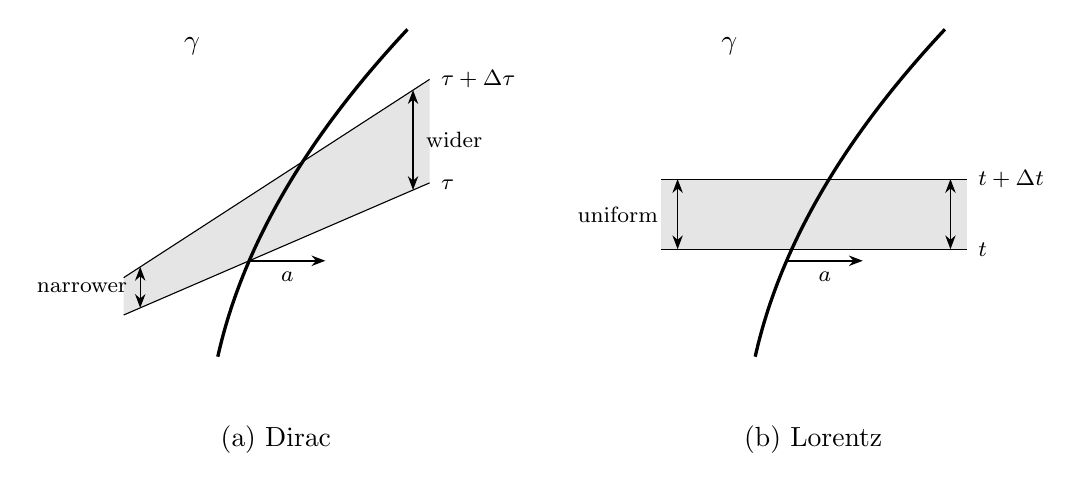
\begin{tikzpicture}[>={Stealth[length=5pt]},scale=2.1,line join=round]

%% ---------------- panel (a): the particle's own simultaneity ----------
\begin{scope}
  \fill[gray!20] (-0.5,0.872) -- (1.35,1.671) -- (1.35,2.297) -- (-0.5,1.098)
     -- cycle;
  %% the two rest-frame slices
  \draw (-0.5,0.872) -- (1.35,1.671);
  \draw (-0.5,1.098) -- (1.35,2.297);
  \node[right,font=\footnotesize] at (1.36,1.66) {$\tau$};
  \node[right,font=\footnotesize] at (1.36,2.30) {$\tau+\Delta\tau$};
  %% world line
  \draw[very thick] plot[domain=0.62:2.6,samples=60,smooth]
       ({0.18*\x*\x},\x);
  \node[left] at (0.02,2.5) {$\gamma$};
  %% acceleration
  \draw[->,thick] (0.259,1.2) -- (0.72,1.2);
  \node[below,font=\footnotesize] at (0.49,1.19) {$a$};
  %% the gap, measured at both ends
  \draw[<->] (-0.4,0.915) -- (-0.4,1.163);
  \draw[<->] (1.25,1.628) -- (1.25,2.232);
  \node[left,font=\footnotesize]  at (-0.42,1.04) {narrower};
  \node[right,font=\footnotesize] at (1.27,1.93) {wider};
  \node at (0.42,0.12) {(a) Dirac};
\end{scope}

%% ---------------- panel (b): constant time in one frame ---------------
\begin{scope}[xshift=3.25cm]
  \fill[gray!20] (-0.5,1.27) rectangle (1.35,1.694);
  \draw (-0.5,1.27)  -- (1.35,1.27);
  \draw (-0.5,1.694) -- (1.35,1.694);
  \node[right,font=\footnotesize] at (1.36,1.27)  {$t$};
  \node[right,font=\footnotesize] at (1.36,1.694) {$t+\Delta t$};
  \draw[very thick] plot[domain=0.62:2.6,samples=60,smooth]
       ({0.18*\x*\x},\x);
  \node[left] at (0.02,2.5) {$\gamma$};
  \draw[->,thick] (0.259,1.2) -- (0.72,1.2);
  \node[below,font=\footnotesize] at (0.49,1.19) {$a$};
  \draw[<->] (-0.4,1.27) -- (-0.4,1.694);
  \draw[<->] (1.25,1.27) -- (1.25,1.694);
  \node[left,font=\footnotesize]  at (-0.46,1.48) {uniform};
  \node at (0.42,0.12) {(b) Lorentz};
\end{scope}

\end{tikzpicture}
\caption{Where the $4/3$ goes. Both panels show the same accelerating world
line $\gamma$ and the same slab of it, and differ only in what is being called
``at the same moment''. \emph{(a)} Dirac's tube is built from the particle's own
succession of rest frames. Because the velocity changes along $\gamma$,
successive slices are not parallel: they fan open on the side the particle is
accelerating towards, and the slab is wider there. That fanning is the factor
$1+\varepsilon\,a\cdot n$ of Eq.~(\ref{eq:tubeelement}). \emph{(b)} Collecting
field momentum at constant time in one chosen frame gives parallel slices and a
slab of uniform thickness, with no such factor. The wedge by which the two
shaded regions differ is worth exactly one third of the electromagnetic mass,
which is the whole of the discrepancy between Eqs.~(\ref{eq:massren}) and
(\ref{eq:divterm}).
\label{fig:simultaneity}}
\end{figure}
.
%% Needs tikz with the arrows.meta library, loaded in the main preamble.
%%
%% Geometry: the world line is x = 0.18 t^2, so the velocity at time t is
%% v = 0.36 t. In an (x,t) diagram the simultaneity line of the instantaneous
%% rest frame at an event has slope dt/dx = v there, so the two slices drawn
%% in panel (a) have slopes 0.432 and 0.648 and cannot be parallel. Every
%% number below follows from those two lines; nothing is drawn by eye.

\begin{figure}[htb]
\centering
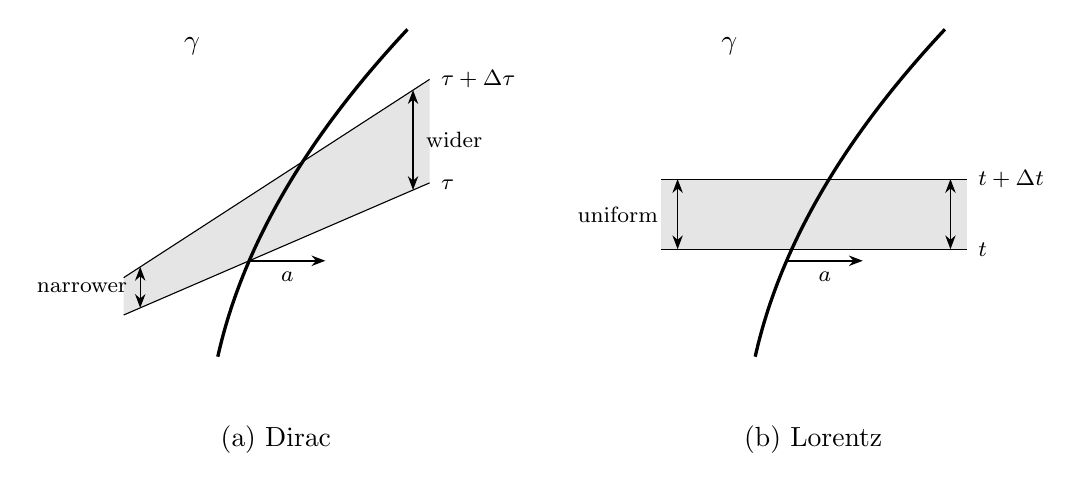
\begin{tikzpicture}[>={Stealth[length=5pt]},scale=2.1,line join=round]

%% ---------------- panel (a): the particle's own simultaneity ----------
\begin{scope}
  \fill[gray!20] (-0.5,0.872) -- (1.35,1.671) -- (1.35,2.297) -- (-0.5,1.098)
     -- cycle;
  %% the two rest-frame slices
  \draw (-0.5,0.872) -- (1.35,1.671);
  \draw (-0.5,1.098) -- (1.35,2.297);
  \node[right,font=\footnotesize] at (1.36,1.66) {$\tau$};
  \node[right,font=\footnotesize] at (1.36,2.30) {$\tau+\Delta\tau$};
  %% world line
  \draw[very thick] plot[domain=0.62:2.6,samples=60,smooth]
       ({0.18*\x*\x},\x);
  \node[left] at (0.02,2.5) {$\gamma$};
  %% acceleration
  \draw[->,thick] (0.259,1.2) -- (0.72,1.2);
  \node[below,font=\footnotesize] at (0.49,1.19) {$a$};
  %% the gap, measured at both ends
  \draw[<->] (-0.4,0.915) -- (-0.4,1.163);
  \draw[<->] (1.25,1.628) -- (1.25,2.232);
  \node[left,font=\footnotesize]  at (-0.42,1.04) {narrower};
  \node[right,font=\footnotesize] at (1.27,1.93) {wider};
  \node at (0.42,0.12) {(a) Dirac};
\end{scope}

%% ---------------- panel (b): constant time in one frame ---------------
\begin{scope}[xshift=3.25cm]
  \fill[gray!20] (-0.5,1.27) rectangle (1.35,1.694);
  \draw (-0.5,1.27)  -- (1.35,1.27);
  \draw (-0.5,1.694) -- (1.35,1.694);
  \node[right,font=\footnotesize] at (1.36,1.27)  {$t$};
  \node[right,font=\footnotesize] at (1.36,1.694) {$t+\Delta t$};
  \draw[very thick] plot[domain=0.62:2.6,samples=60,smooth]
       ({0.18*\x*\x},\x);
  \node[left] at (0.02,2.5) {$\gamma$};
  \draw[->,thick] (0.259,1.2) -- (0.72,1.2);
  \node[below,font=\footnotesize] at (0.49,1.19) {$a$};
  \draw[<->] (-0.4,1.27) -- (-0.4,1.694);
  \draw[<->] (1.25,1.27) -- (1.25,1.694);
  \node[left,font=\footnotesize]  at (-0.46,1.48) {uniform};
  \node at (0.42,0.12) {(b) Lorentz};
\end{scope}

\end{tikzpicture}
\caption{Where the $4/3$ goes. Both panels show the same accelerating world
line $\gamma$ and the same slab of it, and differ only in what is being called
``at the same moment''. \emph{(a)} Dirac's tube is built from the particle's own
succession of rest frames. Because the velocity changes along $\gamma$,
successive slices are not parallel: they fan open on the side the particle is
accelerating towards, and the slab is wider there. That fanning is the factor
$1+\varepsilon\,a\cdot n$ of Eq.~(\ref{eq:tubeelement}). \emph{(b)} Collecting
field momentum at constant time in one chosen frame gives parallel slices and a
slab of uniform thickness, with no such factor. The wedge by which the two
shaded regions differ is worth exactly one third of the electromagnetic mass,
which is the whole of the discrepancy between Eqs.~(\ref{eq:massren}) and
(\ref{eq:divterm}).
\label{fig:simultaneity}}
\end{figure}


Two products of Eq.~(\ref{eq:nearfield}) reach the required order. Take the
Coulomb term against itself first.
\begin{equation}
T^{ij}n_j\Big|_{\rm CC}
= \frac{1}{4\pi}\frac{e^2}{\varepsilon^4}
\left[n^in^j - \tfrac12\delta^{ij}\right]n^j
= \frac{e^2}{8\pi\varepsilon^4}\,n^i .
\label{eq:CC}
\end{equation}
At order $\varepsilon^{-2}$ this integrates to nothing, since
$\oint n^i d\Omega = 0$. An isotropic Coulomb field pushes equally in every
direction. Against the tilt factor it survives:
\begin{equation}
-\oint \frac{e^2}{8\pi\varepsilon^4}\,n^i\,
\varepsilon^3(a\cdot n)\,d\Omega
= -\frac{e^2}{8\pi\varepsilon}\cdot\frac{4\pi}{3}a^i
= -\frac{e^2}{6\varepsilon}\,a^i .
\label{eq:CCtilt}
\end{equation}
The second product is the Coulomb term against the acceleration field, which is
the one a sphere would have too:
\begin{equation}
-\oint\frac{1}{4\pi}
\left[-\frac{e^2}{2\varepsilon^3}a^i
-\frac{e^2}{2\varepsilon^3}(a\cdot n)n^i\right]\varepsilon^2 d\Omega
= \frac{e^2}{2\varepsilon}\left(1+\tfrac13\right)a^i
= \frac{2e^2}{3\varepsilon}\,a^i .
\label{eq:CA}
\end{equation}
Writing $U_0 = e^2/2\varepsilon$ for the electrostatic energy of a shell of
radius $\varepsilon$, the coefficient here is $4U_0/3$: the same $4/3$ the
sphere produced in Sec.~\ref{sec:lorentzmodel}. It is arrived at in the same
way, by ignoring the tilt.

Adding Eqs.~(\ref{eq:CCtilt}) and (\ref{eq:CA}),
\begin{equation}
\frac{dP^i}{d\tau}\bigg|_{\rm div}
= \left(\frac{2}{3}-\frac{1}{6}\right)\frac{e^2}{\varepsilon}\,a^i
= \frac{e^2}{2\varepsilon}\,a^i = U_0\,a^i .
\label{eq:divterm}
\end{equation}

The coefficient is $1$, not $4/3$, and the two derivations in these notes
therefore disagree about the electromagnetic mass:
Eq.~(\ref{eq:massren}) absorbed $4U_0/3c^2$, while Eq.~(\ref{eq:divterm})
absorbs $U_0/c^2$. Neither contains an error, and it is worth being clear about
what the disagreement is.

Section~\ref{sec:lorentzmodel} recorded the $4/3$ as the mark of having counted
the electromagnetic stress while omitting whatever holds the sphere together.
Dirac's calculation has no sphere to hold together and no binding stress to
omit, and it returns $U_0/c^2$. What produces the difference is the tilt factor
of Eq.~(\ref{eq:tubeelement}), and the tilt factor is a statement about
simultaneity. Lorentz gathers the field momentum on a hyperplane of constant
time in one chosen frame. Dirac gathers it on a surface assembled from the
particle's own succession of rest frames. The gap between those two ways of
deciding what counts as ``at the same moment'' is precisely the missing third.

The $4/3$ was never a statement about electrons. It was a statement about a
choice of simultaneity, and it disappears as soon as the choice is made
covariantly.

\subsubsection{The finite term, and two checks}
\label{sec:finiteterm}

The cross of the Coulomb field with the radiative term
$\tfrac{2e}{3}\dot{\mathbf a}$ gives, after the first and third pieces of
$T^{ij}n_j$ cancel against each other,
\begin{equation}
-\oint\frac{1}{4\pi}\frac{2e^2}{3\varepsilon^2}\,\dot a^i\,
\varepsilon^2\,d\Omega = -\frac{2e^2}{3}\,\dot a^i .
\label{eq:finiteterm}
\end{equation}
The finite pieces not written out are the acceleration field against itself,
$\mathbf B$ against itself, and the tilt correction to Eq.~(\ref{eq:CA}). They
contain no $\dot a$, and assemble into the term along $u^\mu$ that
$u\cdot dP/d\tau = 0$ requires. Restoring $c$,
\begin{equation}
\frac{dP^\mu}{d\tau}
= \frac{e^2}{2\varepsilon c^2}\,a^\mu
- \frac{2e^2}{3c^3}\left(\dot a^\mu - u^\mu a^\beta a_\beta\right),
\label{eq:tuberesult}
\end{equation}
$P^\mu$ being the four-momentum carried out of the tube.

Two things can be checked without redoing anything. Contracting
Eq.~(\ref{eq:tuberesult}) with $u_\mu$, and using $u\cdot u=-1$ and
$u\cdot\dot a = -a\cdot a$, gives zero, as it must. And the component along
$u^\mu$ is $(2e^2/3c^3)\,a\cdot a$, the Larmor power. Thus the radiated energy
is present with the coefficient that Sec.~\ref{sec:enbal} obtained from energy
balance, by an argument that never mentioned a tube.

What Eq.~(\ref{eq:tuberesult}) is not is an equation of motion. It records how
much four-momentum the \emph{field} carries out of the tube. Turning that into a
statement about the particle requires saying what the particle's own
four-momentum is, and nothing in the calculation supplies it. That freedom is
the subject of Sec.~\ref{sec:Bmu}.

\subsection{The undetermined four-vector $B^\mu$}
\label{sec:Bmu}

Total four-momentum is conserved, so the particle's own four-momentum changes at
the rate at which the external field supplies it, less the rate at which the
field carries it out of the tube,
\begin{equation}
\frac{dP_{\rm mech}^\mu}{d\tau} = F^\mu_{\rm ext} - \frac{dP^\mu}{d\tau},
\label{eq:balance}
\end{equation}
with $dP^\mu/d\tau$ given by Eq.~(\ref{eq:tuberesult}). Everything on the right
is known. The left is not, because nothing computed so far says what
$P_{\rm mech}^\mu$ is.

This is the bill for the trick of Sec.~\ref{sec:tubeindep}. The tube integral
was arranged to be insensitive to what lies inside it. That insensitivity is
exactly why the divergent self-field never had to be evaluated. But the
particle lies inside it. The construction is silent about the interior by
design, and it is silent about the particle's own momentum for the same reason.
So a form has to be put in by hand:
\begin{equation}
P_{\rm mech}^\mu = m_0 u^\mu + B^\mu ,
\label{eq:Pmech}
\end{equation}
with $B^\mu$ undetermined.

One condition is available. Since $u\cdot u = -1$ throughout, $u\cdot a = 0$, and
contracting Eq.~(\ref{eq:balance}) with $u_\mu$ must therefore give an identity.
The Lorentz force is orthogonal to $u$, and $u\cdot dP/d\tau = 0$ was checked in
Sec.~\ref{sec:finiteterm}, and $m_0\,u\cdot a = 0$. What remains is
\begin{equation}
u_\mu\,\frac{dB^\mu}{d\tau} = 0 .
\label{eq:Bcond}
\end{equation}
This says no more than that whatever force $B^\mu$ contributes must be
orthogonal to the four-velocity, which is a requirement on any force term in a
relativistic equation of motion. It is the only condition the tube construction
imposes, though not the only one that has been imposed on $B^\mu$ in the
literature: \citet{eliezer1947} requires in addition that
$v_\lambda P_{\rm mech}^\mu - v^\mu P_{{\rm mech}\,\lambda}$ be a perfect
differential, which is what forces the series of Sec.~\ref{sec:Bexpand} to
contain only even derivatives.

It is a very weak condition. One scalar equation restricts four functions, so
three functions of $\tau$ remain free at every instant. Dirac's choice is the
simplest solution,
\begin{equation}
B^\mu = k\,u^\mu, \qquad k = \text{const},
\label{eq:Bdirac}
\end{equation}
for which $dB^\mu/d\tau = k\,a^\mu$ and Eq.~(\ref{eq:Bcond}) holds
automatically. Substituting Eqs.~(\ref{eq:Pmech}) and (\ref{eq:Bdirac}) into
Eq.~(\ref{eq:balance}) with Eq.~(\ref{eq:tuberesult}),
\begin{equation}
\left(m_0 + k + \frac{e^2}{2\varepsilon c^2}\right)a^\mu
= F^\mu_{\rm ext} + \frac{2e^2}{3c^3}\left(\dot a^\mu - u^\mu a^\beta a_\beta\right),
\label{eq:preLD}
\end{equation}
and the entire content of Dirac's choice is visible in the bracket: $k$ appears
only added to $m_0$ and to the divergent $e^2/2\varepsilon c^2$. Choosing
$B^\mu = k u^\mu$ is choosing to add nothing to the dynamics. It shifts a mass,
and the mass is not observable separately in any case, since only the sum
\begin{equation}
m = m_0 + k + \frac{e^2}{2\varepsilon c^2}
\label{eq:massren2}
\end{equation}
appears. Holding $m$ finite as $\varepsilon\to0$ requires $m_0 + k \to -\infty$,
which should be recorded plainly. The bare mass is negatively infinite, and the
observed mass is the residue of a cancellation between two quantities. Neither
quantity is separately meaningful.

Two things follow, and they point in opposite directions.

The first is that the derivation has not determined the equation of motion. It
has determined it \emph{given} Eq.~(\ref{eq:Bdirac}), and
Eq.~(\ref{eq:Bdirac}) was chosen for simplicity, not derived. Any
\begin{equation}
B^\mu = P_0\,u^\mu + P_1\,a^\mu + P_2\,\dot a^\mu + \cdots
\label{eq:Bgeneral}
\end{equation}
whose derivative is orthogonal to $u$ is equally admissible, and each choice
yields a different equation of motion. It is generally of higher order, since
each extra term carries another derivative. Dirac himself put it as a choice of the
simplest form rather than as a result. Section~\ref{sec:eliezer} takes that door
seriously and walks through it.

The second is that the freedom is less mysterious than the notation makes it
look, because a particular choice of $B^\mu$ is nothing but a choice of what to
call the particle's momentum. Suppose one posits, instead of
Eq.~(\ref{eq:Bdirac}),
\begin{equation}
P_{\rm mech}^\mu = m_0 u^\mu + C\,\frac{e^2}{c^3}a^\mu
\label{eq:PmechC}
\end{equation}
and asks what $C$ must be if the field side is to contain only the irreversible
radiated momentum. In that bookkeeping the Schott piece has been moved from the
field momentum into $P_{\rm mech}^\mu$. Contracting the source-free balance with
$u_\mu$, the mechanical side gives
$u\cdot(m_0 a + Ce^2\dot a/c^3) = -Ce^2\,a\cdot a/c^3$. The remaining radiative
field piece contributes $-\tfrac23 e^2 a\cdot a/c^3$, so the two cancel only if
\begin{equation}
C = -\tfrac23 .
\label{eq:Cvalue}
\end{equation}
So orthogonality does fix the coefficient, once the \emph{form} has been assumed.
This is the same situation as before, wearing different clothes. What is
worth noticing is the object it fixes. The extra piece of the momentum is
$-\tfrac23 e^2 a^\mu/c^3$, which is the Schott momentum. It is the same quantity that
appeared in Sec.~\ref{sec:enbal} as the boundary term
$(2e^2/3c^3)\,\dot{\mathbf v}\cdot\mathbf v$ that the energy-balance derivation
was permitted to discard. It was discarded there by assuming periodic motion.
Here it cannot be discarded, and it has to be carried as part of what the
particle owns.

\subsection{The equation}
\label{sec:LDeq}

Absorbing the mass as in Eq.~(\ref{eq:massren2}), Eq.~(\ref{eq:preLD}) is the
Lorentz--Dirac equation,
\begin{equation}
\boxed{\;ma^\alpha = \Fext + \frac{2e^2}{3c^3}
\left(\delta^\alpha{}_\beta + u^\alpha u_\beta\right)\dot a^\beta\;}
\tag{LD}
\label{eq:LD}
\end{equation}
the projector $\delta^\alpha{}_\beta + u^\alpha u_\beta$ being the compact way of
writing $\dot a^\alpha - u^\alpha a\cdot a$, and enforcing $u\cdot a = 0$ term by
term.

The reaction force has two pieces and they are not the same kind of thing. The
piece $\tfrac{2e^2}{3c^3}\dot a^\alpha$ is the Schott term. It is a total
derivative, it changes sign with $\dot a$, and it is not radiation. It is
momentum lent to the near field and returned. The piece
$-\tfrac{2e^2}{3c^3}u^\alpha a\cdot a$ points along the four-velocity, never
changes sign, and is exactly the Larmor power carried off, as
Sec.~\ref{sec:finiteterm} verified. Only the second is irreversible. Almost
every puzzle in Sec.~\ref{sec:LDdisc} is a puzzle about the first. The radiated
power and the work done by the reaction force fail to match instant by instant.
Uniform acceleration radiates while feeling no reaction at all.

It is worth stating what this derivation did and did not buy, since the same
equation was very nearly written down in Sec.~\ref{sec:lorentzmodel} by
Landau and Lifshitz's two-line covariantization, Eq.~(\ref{eq:LLcov}). What is
new is not the form. Covariance and $u\cdot a = 0$ fix the form almost by
themselves, and the coefficient $2e^2/3c^3$ was already fixed by the
nonrelativistic limit. What is new is, first, that no extended body was needed
and therefore no binding stress was omitted, which is why the electromagnetic
mass came out as $U_0/c^2$ rather than $4U_0/3c^2$. Second, the freedom left
over has been made explicit rather than hidden, in the shape of
Eq.~(\ref{eq:Bgeneral}). A derivation that tells you exactly which of its
conclusions were choices is worth more than one that reaches the same equation
silently.

What the derivation did not buy is any improvement in the behaviour of the
solutions. Equation~(\ref{eq:LD}) still contains $\dot a$, so it is still of
third order in the position, and Sec.~\ref{sec:runaway} already showed what that
implies. Section~\ref{sec:LDdisc} works out the consequences.

\subsection{The other route: separating the singular part}
\label{sec:sepsing}

%% figures/fig-retadv.tex -- Figure for Sec. 2.4.
%% Pulled into notes.tex with %% figures/fig-retadv.tex -- Figure for Sec. 2.4.
%% Pulled into notes.tex with %% figures/fig-retadv.tex -- Figure for Sec. 2.4.
%% Pulled into notes.tex with \input{figures/fig-retadv}.
%% Needs tikz with the arrows.meta library, loaded in the main preamble.
%%
%% Same world line as fig-simultaneity.tex, x = 0.18 t^2, so that the two
%% figures can be read against each other. The intersections of the light cone
%% through the field point with the world line are solved exactly, not placed
%% by eye. For a field point at (X,T) the null condition 0.18 t^2 = X -+ (T - t)
%% is a quadratic in t:
%%
%%   panel (a), X = 0.95, T = 1.6:
%%       retarded   0.18 t^2 - t + 0.65 = 0  ->  t = 0.7517, x = 0.1017
%%       advanced   0.18 t^2 + t - 2.55 = 0  ->  t = 1.9000, x = 0.6498
%%   panel (b), X = 0.52, T = 1.6:
%%       retarded   0.18 t^2 - t + 1.08 = 0  ->  t = 1.4678, x = 0.3878
%%       advanced   0.18 t^2 + t - 2.12 = 0  ->  t = 1.6374, x = 0.4826
%%
%% Both null rays are therefore at 45 degrees by construction, and the merging
%% of u and v in panel (b) is a computed fact about those roots.

\begin{figure}[htb]
\centering
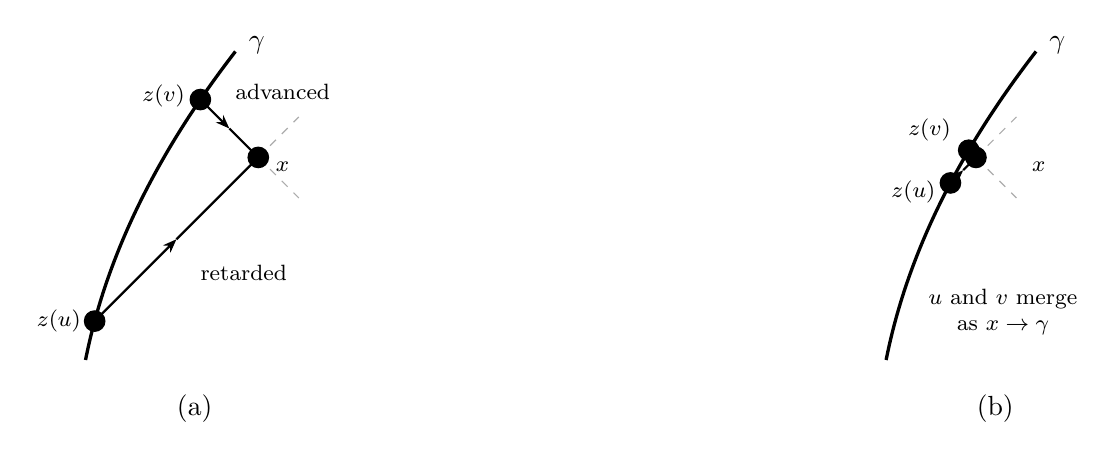
\begin{tikzpicture}[>={Stealth[length=5pt]},scale=2.45,line join=round]

%% ---------------- panel (a): a field point off the world line ----------
\begin{scope}
  %% short stubs marking the light cone through x
  \draw[dashed,gray!65] (0.95,1.6) -- (1.16,1.81);
  \draw[dashed,gray!65] (0.95,1.6) -- (1.16,1.39);
  %% world line
  \draw[very thick] plot[domain=0.55:2.15,samples=70,smooth]
       ({0.18*\x*\x},\x);
  \node[right] at (0.85,2.18) {$\gamma$};
  %% the two null rays that matter
  \draw[->,thick] (0.1017,0.7517) -- (0.5259,1.1759);
  \draw[thick] (0.5259,1.1759) -- (0.95,1.6);
  \draw[->,thick] (0.6498,1.9000) -- (0.7999,1.7499);
  \draw[thick] (0.7999,1.7499) -- (0.95,1.6);
  %% events
  \fill (0.1017,0.7517) circle (1.6pt);
  \node[left,font=\footnotesize] at (0.08,0.7517) {$z(u)$};
  \fill (0.6498,1.9000) circle (1.6pt);
  \node[left,font=\footnotesize] at (0.62,1.92) {$z(v)$};
  \fill (0.95,1.6) circle (1.6pt);
  \node[right,font=\footnotesize] at (0.99,1.55) {$x$};
  %% which ray is which, set level and clear of the rays
  \node[right,font=\footnotesize] at (0.60,1.00) {retarded};
  \node[right,font=\footnotesize] at (0.78,1.94) {advanced};
  \node at (0.62,0.30) {(a)};
\end{scope}

%% ---------------- panel (b): the field point brought close --------------
\begin{scope}[xshift=4.15cm]
  \draw[dashed,gray!65] (0.52,1.6) -- (0.73,1.81);
  \draw[dashed,gray!65] (0.52,1.6) -- (0.73,1.39);
  \draw[very thick] plot[domain=0.55:2.15,samples=70,smooth]
       ({0.18*\x*\x},\x);
  \node[right] at (0.85,2.18) {$\gamma$};
  \draw[->,thick] (0.3878,1.4678) -- (0.4539,1.5339);
  \draw[thick] (0.4539,1.5339) -- (0.52,1.6);
  \draw[->,thick] (0.4826,1.6374) -- (0.5013,1.6187);
  \draw[thick] (0.5013,1.6187) -- (0.52,1.6);
  \fill (0.3878,1.4678) circle (1.6pt);
  \node[left,font=\footnotesize] at (0.36,1.42) {$z(u)$};
  \fill (0.4826,1.6374) circle (1.6pt);
  \node[left,font=\footnotesize] at (0.44,1.74) {$z(v)$};
  \fill (0.52,1.6) circle (1.6pt);
  \node[right,font=\footnotesize] at (0.76,1.55) {$x$};
  \node[align=center,font=\footnotesize] at (0.66,0.80)
       {$u$ and $v$ merge\\as $x\to\gamma$};
  \node at (0.62,0.30) {(b)};
\end{scope}

\end{tikzpicture}
\caption{What the retarded and advanced potentials are, geometrically. The light
cone through a field point $x$ meets the world line twice: once in the past, at
$z(u)$, and once in the future, at $z(v)$. The first gives $A_{\rm ret}$, the
second $A_{\rm adv}$. \emph{(a)} For $x$ well off the world line the two events
are far apart, and only the retarded one is causally admissible. \emph{(b)} As
$x$ is brought towards the world line the two roots approach each other and both
approach the same event. Both potentials diverge there, at the same rate and
with the same coefficient, because both are being sourced by the same piece of
the same world line; that is why the singular parts cancel in the difference
$\tfrac12(A_{\rm ret}-A_{\rm adv})$ and survive undiminished in the sum
$\tfrac12(A_{\rm ret}+A_{\rm adv})$. Equation~(\ref{eq:retadvsplit}) splits them
where it does for this reason and no other.
\label{fig:retadv}}
\end{figure}
.
%% Needs tikz with the arrows.meta library, loaded in the main preamble.
%%
%% Same world line as fig-simultaneity.tex, x = 0.18 t^2, so that the two
%% figures can be read against each other. The intersections of the light cone
%% through the field point with the world line are solved exactly, not placed
%% by eye. For a field point at (X,T) the null condition 0.18 t^2 = X -+ (T - t)
%% is a quadratic in t:
%%
%%   panel (a), X = 0.95, T = 1.6:
%%       retarded   0.18 t^2 - t + 0.65 = 0  ->  t = 0.7517, x = 0.1017
%%       advanced   0.18 t^2 + t - 2.55 = 0  ->  t = 1.9000, x = 0.6498
%%   panel (b), X = 0.52, T = 1.6:
%%       retarded   0.18 t^2 - t + 1.08 = 0  ->  t = 1.4678, x = 0.3878
%%       advanced   0.18 t^2 + t - 2.12 = 0  ->  t = 1.6374, x = 0.4826
%%
%% Both null rays are therefore at 45 degrees by construction, and the merging
%% of u and v in panel (b) is a computed fact about those roots.

\begin{figure}[htb]
\centering
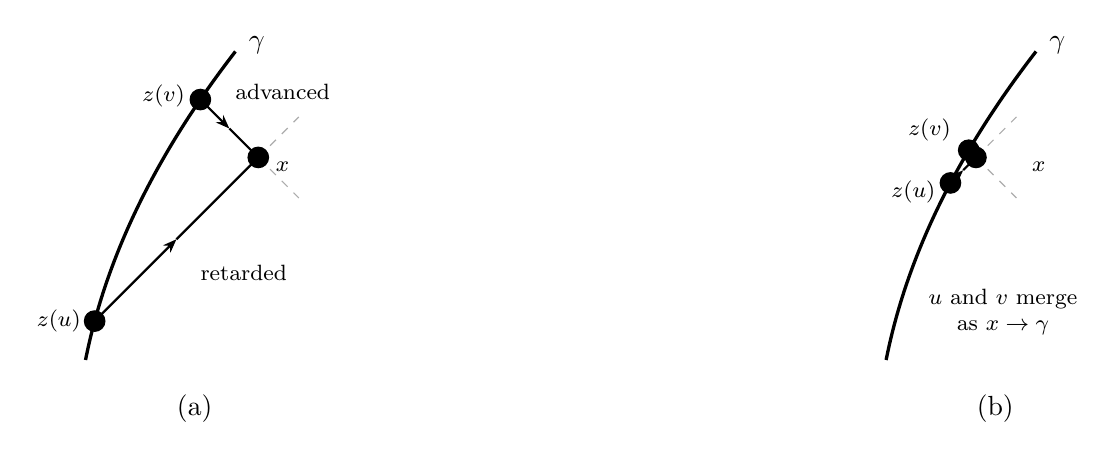
\begin{tikzpicture}[>={Stealth[length=5pt]},scale=2.45,line join=round]

%% ---------------- panel (a): a field point off the world line ----------
\begin{scope}
  %% short stubs marking the light cone through x
  \draw[dashed,gray!65] (0.95,1.6) -- (1.16,1.81);
  \draw[dashed,gray!65] (0.95,1.6) -- (1.16,1.39);
  %% world line
  \draw[very thick] plot[domain=0.55:2.15,samples=70,smooth]
       ({0.18*\x*\x},\x);
  \node[right] at (0.85,2.18) {$\gamma$};
  %% the two null rays that matter
  \draw[->,thick] (0.1017,0.7517) -- (0.5259,1.1759);
  \draw[thick] (0.5259,1.1759) -- (0.95,1.6);
  \draw[->,thick] (0.6498,1.9000) -- (0.7999,1.7499);
  \draw[thick] (0.7999,1.7499) -- (0.95,1.6);
  %% events
  \fill (0.1017,0.7517) circle (1.6pt);
  \node[left,font=\footnotesize] at (0.08,0.7517) {$z(u)$};
  \fill (0.6498,1.9000) circle (1.6pt);
  \node[left,font=\footnotesize] at (0.62,1.92) {$z(v)$};
  \fill (0.95,1.6) circle (1.6pt);
  \node[right,font=\footnotesize] at (0.99,1.55) {$x$};
  %% which ray is which, set level and clear of the rays
  \node[right,font=\footnotesize] at (0.60,1.00) {retarded};
  \node[right,font=\footnotesize] at (0.78,1.94) {advanced};
  \node at (0.62,0.30) {(a)};
\end{scope}

%% ---------------- panel (b): the field point brought close --------------
\begin{scope}[xshift=4.15cm]
  \draw[dashed,gray!65] (0.52,1.6) -- (0.73,1.81);
  \draw[dashed,gray!65] (0.52,1.6) -- (0.73,1.39);
  \draw[very thick] plot[domain=0.55:2.15,samples=70,smooth]
       ({0.18*\x*\x},\x);
  \node[right] at (0.85,2.18) {$\gamma$};
  \draw[->,thick] (0.3878,1.4678) -- (0.4539,1.5339);
  \draw[thick] (0.4539,1.5339) -- (0.52,1.6);
  \draw[->,thick] (0.4826,1.6374) -- (0.5013,1.6187);
  \draw[thick] (0.5013,1.6187) -- (0.52,1.6);
  \fill (0.3878,1.4678) circle (1.6pt);
  \node[left,font=\footnotesize] at (0.36,1.42) {$z(u)$};
  \fill (0.4826,1.6374) circle (1.6pt);
  \node[left,font=\footnotesize] at (0.44,1.74) {$z(v)$};
  \fill (0.52,1.6) circle (1.6pt);
  \node[right,font=\footnotesize] at (0.76,1.55) {$x$};
  \node[align=center,font=\footnotesize] at (0.66,0.80)
       {$u$ and $v$ merge\\as $x\to\gamma$};
  \node at (0.62,0.30) {(b)};
\end{scope}

\end{tikzpicture}
\caption{What the retarded and advanced potentials are, geometrically. The light
cone through a field point $x$ meets the world line twice: once in the past, at
$z(u)$, and once in the future, at $z(v)$. The first gives $A_{\rm ret}$, the
second $A_{\rm adv}$. \emph{(a)} For $x$ well off the world line the two events
are far apart, and only the retarded one is causally admissible. \emph{(b)} As
$x$ is brought towards the world line the two roots approach each other and both
approach the same event. Both potentials diverge there, at the same rate and
with the same coefficient, because both are being sourced by the same piece of
the same world line; that is why the singular parts cancel in the difference
$\tfrac12(A_{\rm ret}-A_{\rm adv})$ and survive undiminished in the sum
$\tfrac12(A_{\rm ret}+A_{\rm adv})$. Equation~(\ref{eq:retadvsplit}) splits them
where it does for this reason and no other.
\label{fig:retadv}}
\end{figure}
.
%% Needs tikz with the arrows.meta library, loaded in the main preamble.
%%
%% Same world line as fig-simultaneity.tex, x = 0.18 t^2, so that the two
%% figures can be read against each other. The intersections of the light cone
%% through the field point with the world line are solved exactly, not placed
%% by eye. For a field point at (X,T) the null condition 0.18 t^2 = X -+ (T - t)
%% is a quadratic in t:
%%
%%   panel (a), X = 0.95, T = 1.6:
%%       retarded   0.18 t^2 - t + 0.65 = 0  ->  t = 0.7517, x = 0.1017
%%       advanced   0.18 t^2 + t - 2.55 = 0  ->  t = 1.9000, x = 0.6498
%%   panel (b), X = 0.52, T = 1.6:
%%       retarded   0.18 t^2 - t + 1.08 = 0  ->  t = 1.4678, x = 0.3878
%%       advanced   0.18 t^2 + t - 2.12 = 0  ->  t = 1.6374, x = 0.4826
%%
%% Both null rays are therefore at 45 degrees by construction, and the merging
%% of u and v in panel (b) is a computed fact about those roots.

\begin{figure}[htb]
\centering
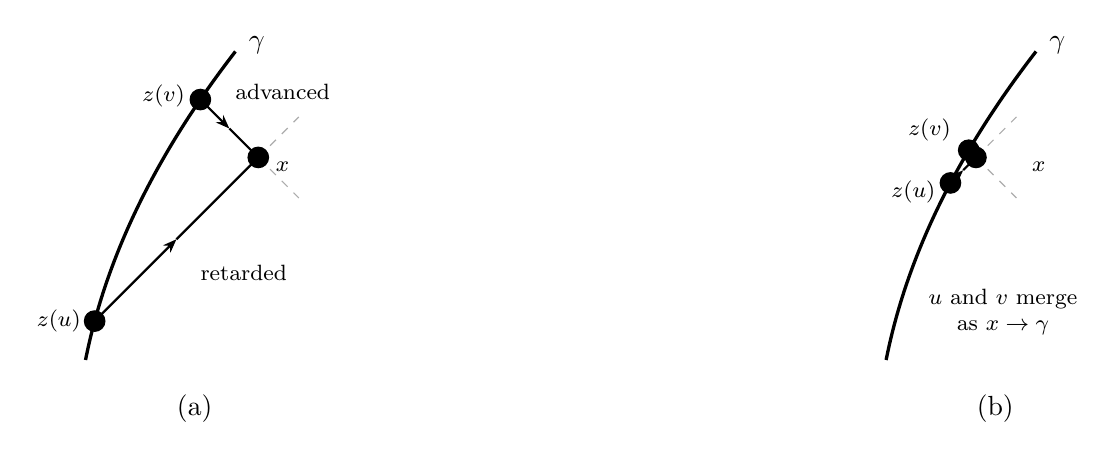
\begin{tikzpicture}[>={Stealth[length=5pt]},scale=2.45,line join=round]

%% ---------------- panel (a): a field point off the world line ----------
\begin{scope}
  %% short stubs marking the light cone through x
  \draw[dashed,gray!65] (0.95,1.6) -- (1.16,1.81);
  \draw[dashed,gray!65] (0.95,1.6) -- (1.16,1.39);
  %% world line
  \draw[very thick] plot[domain=0.55:2.15,samples=70,smooth]
       ({0.18*\x*\x},\x);
  \node[right] at (0.85,2.18) {$\gamma$};
  %% the two null rays that matter
  \draw[->,thick] (0.1017,0.7517) -- (0.5259,1.1759);
  \draw[thick] (0.5259,1.1759) -- (0.95,1.6);
  \draw[->,thick] (0.6498,1.9000) -- (0.7999,1.7499);
  \draw[thick] (0.7999,1.7499) -- (0.95,1.6);
  %% events
  \fill (0.1017,0.7517) circle (1.6pt);
  \node[left,font=\footnotesize] at (0.08,0.7517) {$z(u)$};
  \fill (0.6498,1.9000) circle (1.6pt);
  \node[left,font=\footnotesize] at (0.62,1.92) {$z(v)$};
  \fill (0.95,1.6) circle (1.6pt);
  \node[right,font=\footnotesize] at (0.99,1.55) {$x$};
  %% which ray is which, set level and clear of the rays
  \node[right,font=\footnotesize] at (0.60,1.00) {retarded};
  \node[right,font=\footnotesize] at (0.78,1.94) {advanced};
  \node at (0.62,0.30) {(a)};
\end{scope}

%% ---------------- panel (b): the field point brought close --------------
\begin{scope}[xshift=4.15cm]
  \draw[dashed,gray!65] (0.52,1.6) -- (0.73,1.81);
  \draw[dashed,gray!65] (0.52,1.6) -- (0.73,1.39);
  \draw[very thick] plot[domain=0.55:2.15,samples=70,smooth]
       ({0.18*\x*\x},\x);
  \node[right] at (0.85,2.18) {$\gamma$};
  \draw[->,thick] (0.3878,1.4678) -- (0.4539,1.5339);
  \draw[thick] (0.4539,1.5339) -- (0.52,1.6);
  \draw[->,thick] (0.4826,1.6374) -- (0.5013,1.6187);
  \draw[thick] (0.5013,1.6187) -- (0.52,1.6);
  \fill (0.3878,1.4678) circle (1.6pt);
  \node[left,font=\footnotesize] at (0.36,1.42) {$z(u)$};
  \fill (0.4826,1.6374) circle (1.6pt);
  \node[left,font=\footnotesize] at (0.44,1.74) {$z(v)$};
  \fill (0.52,1.6) circle (1.6pt);
  \node[right,font=\footnotesize] at (0.76,1.55) {$x$};
  \node[align=center,font=\footnotesize] at (0.66,0.80)
       {$u$ and $v$ merge\\as $x\to\gamma$};
  \node at (0.62,0.30) {(b)};
\end{scope}

\end{tikzpicture}
\caption{What the retarded and advanced potentials are, geometrically. The light
cone through a field point $x$ meets the world line twice: once in the past, at
$z(u)$, and once in the future, at $z(v)$. The first gives $A_{\rm ret}$, the
second $A_{\rm adv}$. \emph{(a)} For $x$ well off the world line the two events
are far apart, and only the retarded one is causally admissible. \emph{(b)} As
$x$ is brought towards the world line the two roots approach each other and both
approach the same event. Both potentials diverge there, at the same rate and
with the same coefficient, because both are being sourced by the same piece of
the same world line; that is why the singular parts cancel in the difference
$\tfrac12(A_{\rm ret}-A_{\rm adv})$ and survive undiminished in the sum
$\tfrac12(A_{\rm ret}+A_{\rm adv})$. Equation~(\ref{eq:retadvsplit}) splits them
where it does for this reason and no other.
\label{fig:retadv}}
\end{figure}


There is a second way through, and it has the opposite character. Dirac's route
declines to ask what force the charge exerts on itself and audits the momentum
instead. This one asks about the force after all, but subtracts, before asking,
the part of the self-field that makes the question meaningless.

The difficulty being addressed is the one stated in Sec.~\ref{sec:lorentz}: at
the electron both the potential and the field tensor are infinite, so the
Lorentz force expression cannot be applied to the self-field. The proposal is to
split the infinite self-field into an ``irrelevant'' singular part, which is
discarded, and a finite ``effective'' part, and then to apply the Lorentz force
law to the effective part alone, in the ordinary way. The discarded piece is
called the singular term, and the procedure is the method of separating the
singular part.

The split that works is between the advanced and retarded potentials. The
advanced potential $A_{\rm adv}$ violates causality and is not a candidate for
the physical field, but it is a perfectly good solution of
$\Box A^\alpha = -4\pi j^\alpha$, and near the world line its singular behaviour
is identical to that of $A_{\rm ret}$. In the difference the singular behaviour
cancels. What is kept and what is thrown away are therefore
\begin{equation}
A^\alpha_{(R)} = \tfrac12\left(\Aret - \Aadv\right),
\qquad
A^\alpha_{(S)} = \tfrac12\left(\Aret + \Aadv\right),
\label{eq:retadvsplit}
\end{equation}
the first being a difference of two solutions of the inhomogeneous equation and
hence a solution of the homogeneous Maxwell equations, regular on the world line,
with a finite Lorentz force
$f^\alpha = e\,F^{(R)\alpha}{}_\beta u^\beta$.

That this reproduces Dirac's answer is the content of the equivalence theorem:

\begin{quote}
The motion obtained from momentum--energy conservation is the same as the motion
produced by the Lorentz force of the potential
$\tfrac12(A_{\rm ret}-A_{\rm adv})$.
\end{quote}

Part of the check is already in hand. The finite term computed in
Sec.~\ref{sec:finiteterm} is precisely $e$ times
$\tfrac12(F_{\rm ret}-F_{\rm adv})$ evaluated on the world line, which is why
the same $2e^2/3c^3$ appeared there. The agreement of the two routes is not an
accident, but neither is it obvious: one of them never evaluates a field at the
particle and the other does nothing else.

Proofs are given by \citet{zhang_zongsui} and, in retarded coordinates, by
\citet{poisson2004}. The version reproduced here is deferred to
Sec.~\ref{sec:equiv}, and it is worth saying why it
gets a section of its own rather than a footnote. Its value is not that it
confirms Eq.~(\ref{eq:LD}) a third time. It is that carrying the proof out makes
visible something the statement conceals: that Eq.~(\ref{eq:retadvsplit}) is a
\emph{choice} of which combination to discard, and that the choice was made on
grounds of convenience. Section~\ref{sec:lk} relaxes it, replacing
Eq.~(\ref{eq:retadvsplit}) by a two-parameter family, and everything in that
section descends from the observation that the split is not forced.

\subsection{The end caps, and where the freedom in $B^\mu$ comes from}
\label{sec:reservations}

One reservation about the derivation remains to be entered, and it turns out not
to be independent of the freedom found in Sec.~\ref{sec:Bmu}.

The region $V$ occupied by the tube between $\tau_1$ and $\tau_2$ is bounded by
the wall $\Sigma_{\rm tube}$ and by two spacelike end caps $C(\tau_1)$ and
$C(\tau_2)$, the discs closing the tube at each end. Conservation applies to the
whole boundary, not to part of it:
\begin{equation}
\int_{C(\tau_2)} T^{\mu\nu}d\Sigma_\nu
- \int_{C(\tau_1)} T^{\mu\nu}d\Sigma_\nu
+ \int_{\Sigma_{\rm tube}} T^{\mu\nu}d\Sigma_\nu
= \int_V T^{\mu\nu}{}_{,\nu}\,dV .
\label{eq:capbalance}
\end{equation}
Both the calculation of Sec.~\ref{sec:tube} and Poisson's shorter version
\citep{poisson2004}
evaluate the third term only. The 2006 text records this and does not pursue it.

The two cap integrals are not incidental. Each is the four-momentum of the field
contained inside the tube at one end,
\begin{equation}
P_{\rm field}^\mu(\tau) = \int_{C(\tau)} T^{\mu\nu}d\Sigma_\nu ,
\label{eq:Pfield}
\end{equation}
so what Eq.~(\ref{eq:capbalance}) says is that the wall integral measures the
change in the field momentum \emph{inside} the tube, and not the change in the
particle's momentum. Those are different quantities, and separating them
requires knowing how the contents of the tube divide between the particle and
its field.

Which is exactly what Sec.~\ref{sec:Bmu} had to put in by hand. If
Eq.~(\ref{eq:Pfield}) could be evaluated, $P_{\rm mech}^\mu$ would follow from it
rather than being posited, Eq.~(\ref{eq:Pmech}) would not be needed, and the
four-vector $B^\mu$ would have no freedom left in it. The arbitrariness in
$B^\mu$ is not a second defect standing alongside the missing caps. It is the
missing caps, seen from the side of the equation of motion.

The caps are omitted because they diverge. On a cap the Coulomb energy density
goes as $e^2/r^4$ against a volume element $r^2dr$, and the momentum density,
carrying one factor of $\mathbf B \sim 1/r$, as $e^2/r^3$; the two radial
integrals
\begin{equation}
\int_0 \frac{dr}{r^2}, \qquad \int_0 \frac{dr}{r}
\label{eq:capdiv}
\end{equation}
diverge at the lower limit, the second only logarithmically but no less fatally.
The field momentum inside the tube is infinite, which is why it cannot be
apportioned, which is why a form for $P_{\rm mech}^\mu$ has to be assumed.

This closes the account of Sec.~\ref{sec:tube} in a way worth stating plainly.
The virtue of the tube construction and its cost are the same property. It works
because it is insensitive to what lies inside it, and it is for that reason
unable to say anything about what lies inside it. The divergence was not
removed. It was moved to a place where it could be ignored, and the price of
ignoring it is one undetermined four-vector.

A further consequence of the same divergence is left aside here. The
stress--energy tensor of the electron's own field curves spacetime, and a
quantity that diverges on the world line curves it without bound, so the
particle is not in Minkowski space and general relativity has nothing to say
about the region where the problem lives. The 2006 text raises this in its
Sec.~4 and builds an ``effective metric'' proposal on it; that material is not
covered in these notes.

%% ===================================================================
\section{The Lorentz--Dirac Equation: Discussion and Solutions}
\label{sec:LDdisc}

Equation~(\ref{eq:LD}) has been derived twice and its freedoms accounted for.
This section asks what it says, and the answer is that it says very nearly
everything the Abraham--Lorentz equation said in Sec.~\ref{sec:lorentz}, in
covariant dress. That is not a small disappointment. Dirac's construction
repaired the derivation --- no extended body, no omitted binding stress, no
$4/3$ --- and left the disease untouched.

\subsection{One-dimensional reduction}
\label{sec:1dreduction}

Restrict the motion to one spatial dimension. The normalization
$u^\alpha u_\alpha = -1$ reads $\dot t^2 - \dot x^2 = 1$, which is solved
identically by the rapidity $q(\tau)$,
\begin{equation}
\dot t = \cosh q, \qquad \dot x = \sinh q ,
\label{eq:rapidity}
\end{equation}
so that $q$ carries the whole of the kinematics and the constraint is disposed
of once and for all. Differentiating,
\begin{equation}
a^\alpha = \dot q\,(\sinh q,\ \cosh q),
\qquad
\dot a^\alpha = \ddot q\,(\sinh q,\ \cosh q)
             + \dot q^{\,2}(\cosh q,\ \sinh q).
\label{eq:rapidityderivs}
\end{equation}
Two things follow at once. First $a\cdot a = \dot q^{\,2}$, so the invariant
acceleration is just $|\dot q|$. Second, and more usefully, the awkward term in
Eq.~(\ref{eq:LD}) collapses:
\begin{equation}
\dot a^\alpha - u^\alpha\, a\cdot a
= \ddot q\,(\sinh q,\ \cosh q),
\label{eq:reactionreduced}
\end{equation}
because the $\dot q^{\,2}$ pieces of $\dot a^\alpha$ and of
$u^\alpha a\cdot a$ are identical and cancel. Both are proportional to the same
vector $(\sinh q,\cosh q)$ that carries $a^\alpha$, so the two components of
Eq.~(\ref{eq:LD}) are not independent: they reduce to a single scalar equation,
\begin{equation}
\dot q - \taunought\,\ddot q = \frac{1}{m}\,f(\tau),
\label{eq:LD1d}
\end{equation}
where $f = eE$ is the scalar force. In the normalization of the 2006 text,
$m=e=c=1$, one has $\taunought = 2/3$ and Eq.~(\ref{eq:LD1d}) is written
$\dot q - \tfrac23\ddot q = F^{01}$.

The reduction is worth pausing on, because it makes the structural point of
Sec.~\ref{sec:runaway} unmissable. Newton's equation in this variable would be
$m\dot q = f$: rapidity rate proportional to force, no more. What
Eq.~(\ref{eq:LD1d}) adds is $\ddot q$, and it adds it with a coefficient
$\taunought$ that is fixed, not adjustable. The equation is first order in the
acceleration $\dot q$, which is to say third order in the position.

\subsection{The free solution and the runaway}
\label{sec:freesol}

Set $f=0$. Equation~(\ref{eq:LD1d}) becomes
$\ddot q = \dot q/\taunought$, whence
\begin{equation}
q = C_1 e^{\tau/\taunought} + C_2
\qquad\text{and}\qquad
\dot t = \cosh\!\left(C_1e^{\tau/\taunought}+C_2\right),
\quad
\dot x = \sinh\!\left(C_1e^{\tau/\taunought}+C_2\right).
\label{eq:runaway}
\end{equation}
In the 2006 normalization this is $q = C_1e^{3\tau/2}+C_2$.

If $C_1\ne 0$ then $q\to\infty$, and since $dx/dt = \tanh q$, the velocity
approaches $c$. A free electron, in an inertial frame, with nothing whatever
acting on it, accelerates itself to the speed of light. The covariant equation
has improved on Eq.~(\ref{eq:AL}) only in the sense that the velocity now
saturates at $c$ rather than growing without bound; the world line is no less
absurd.

If $C_1 = 0$ then $q$ is constant, the electron moves uniformly, and Newton's
first law is recovered. This is the physical solution, and the difficulty is
the one already met in Sec.~\ref{sec:runaway}: nothing selects it. The three
constants of a third-order equation are fixed by three pieces of data, and
position and velocity supply only two. The third is $\dot q(0)$, the initial
acceleration, which the physical situation does not determine and which the
theory offers no way of measuring; and the only value of it that does not lead
to disaster must be imposed from outside.

The impulse problem sharpens this exactly as it did before. With
$f/m = \kappa\,\delta(\tau)$ and the electron moving uniformly beforehand,
integrating Eq.~(\ref{eq:LD1d}) across the pulse and solving on either side
gives, for $\tau>0$,
\begin{equation}
\dot q = -\frac{\kappa}{\taunought}\,e^{\tau/\taunought},
\label{eq:LDimpulse}
\end{equation}
so the acceleration grows without bound after the blow instead of returning to
zero. The problem Sec.~\ref{sec:runaway} found in Lorentz's equation is
untouched by Dirac's. The 2006 text notes that Zhang's treatment of the single
and double pulse \citep{zhang_zongsui} produces solutions of the same form.

\subsection{Dirac's asymptotic condition and the price paid}
\label{sec:asymptotic}

%% figures/fig-preaccel.tex -- Figure for Sec. 3.3.
%% Pulled into notes.tex with %% figures/fig-preaccel.tex -- Figure for Sec. 3.3.
%% Pulled into notes.tex with %% figures/fig-preaccel.tex -- Figure for Sec. 3.3.
%% Pulled into notes.tex with \input{figures/fig-preaccel}.
%% Needs pgfplots, loaded in the main preamble.
%%
%% Both curves solve tau_0 adot - a = -(J/m) delta(t). Integrating across the
%% delta gives a(0+) - a(0-) = -J/(m tau_0), which fixes each branch once one
%% end condition is chosen:
%%
%%   a(t) = 0 for t<0   ->  a = -(J/m tau_0) exp(t/tau_0) for t>0   (runaway)
%%   a(t) = 0 for t>0   ->  a = +(J/m tau_0) exp(t/tau_0) for t<0   (pre-acc.)
%%
%% The two are reflections of each other through the origin, which is the point
%% of drawing them on one axis. Plotted in units of J/(m tau_0).

\begin{figure}[htb]
\centering
\begin{tikzpicture}
\begin{axis}[
  width=11.2cm, height=6.0cm,
  xlabel={$\tau/\taunought$}, ylabel={$a\ \ [\,J/m\taunought\,]$},
  xmin=-3.1, xmax=3.1, ymin=-1.45, ymax=1.45,
  axis lines=middle,
  ytick={-1,1}, yticklabels={,},
  xtick={-3,-2,-1,1,2,3},
  every axis y label/.style={at={(ticklabel* cs:1.0)},anchor=south east},
  every axis x label/.style={at={(ticklabel* cs:1.0)},anchor=north west},
  clip=true, samples=90, font=\footnotesize,
]
  %% the impulse
  \draw[->,thick,gray] (axis cs:0,0) -- (axis cs:0,1.33);
  \node[anchor=west,font=\footnotesize,gray]
       at (axis cs:0.07,1.30) {$J\,\delta(\tau)$};

  %% branch 1: no pre-acceleration, runaway afterwards
  \addplot[domain=-3.1:0,thick] {0};
  \addplot[domain=0:0.38,thick] {-exp(x)};
  \fill (axis cs:0,-1) circle (1.3pt);

  %% branch 2: asymptotic condition, pre-acceleration beforehand
  \addplot[domain=-3.1:0,thick,dashed] {exp(x)};
  \addplot[domain=0:3.1,thick,dashed] {0};
  \fill (axis cs:0,1) circle (1.3pt);

  \node[anchor=west,font=\footnotesize,align=left] at (axis cs:0.55,-0.80)
       {$a(0^-)=0$\\runs away after};
  \node[anchor=east,font=\footnotesize,align=right] at (axis cs:-0.45,0.80)
       {$a(\infty)=0$\\acts before};
\end{axis}
\end{tikzpicture}
\caption{The choice Dirac's asymptotic condition makes. Both curves solve the
same equation with the same impulse, and differ only in which end condition is
imposed. Fixing the acceleration to vanish before the blow, as an
initial-value problem would, gives the solid curve: nothing happens until
$\tau=0$ and the particle then runs away, as in Fig.~\ref{fig:runaway}(b).
Fixing it to vanish at $\tau\to+\infty$ instead gives the dashed curve: the
runaway is gone, the particle ends in uniform motion with exactly the velocity
change $J/m$ that the impulse should produce, and it acquires that velocity
\emph{before} the impulse arrives, over a time of order $\taunought$. The two
branches are reflections of each other through the origin. There is no third
branch, and no choice that avoids both.
\label{fig:preaccel}}
\end{figure}
.
%% Needs pgfplots, loaded in the main preamble.
%%
%% Both curves solve tau_0 adot - a = -(J/m) delta(t). Integrating across the
%% delta gives a(0+) - a(0-) = -J/(m tau_0), which fixes each branch once one
%% end condition is chosen:
%%
%%   a(t) = 0 for t<0   ->  a = -(J/m tau_0) exp(t/tau_0) for t>0   (runaway)
%%   a(t) = 0 for t>0   ->  a = +(J/m tau_0) exp(t/tau_0) for t<0   (pre-acc.)
%%
%% The two are reflections of each other through the origin, which is the point
%% of drawing them on one axis. Plotted in units of J/(m tau_0).

\begin{figure}[htb]
\centering
\begin{tikzpicture}
\begin{axis}[
  width=11.2cm, height=6.0cm,
  xlabel={$\tau/\taunought$}, ylabel={$a\ \ [\,J/m\taunought\,]$},
  xmin=-3.1, xmax=3.1, ymin=-1.45, ymax=1.45,
  axis lines=middle,
  ytick={-1,1}, yticklabels={,},
  xtick={-3,-2,-1,1,2,3},
  every axis y label/.style={at={(ticklabel* cs:1.0)},anchor=south east},
  every axis x label/.style={at={(ticklabel* cs:1.0)},anchor=north west},
  clip=true, samples=90, font=\footnotesize,
]
  %% the impulse
  \draw[->,thick,gray] (axis cs:0,0) -- (axis cs:0,1.33);
  \node[anchor=west,font=\footnotesize,gray]
       at (axis cs:0.07,1.30) {$J\,\delta(\tau)$};

  %% branch 1: no pre-acceleration, runaway afterwards
  \addplot[domain=-3.1:0,thick] {0};
  \addplot[domain=0:0.38,thick] {-exp(x)};
  \fill (axis cs:0,-1) circle (1.3pt);

  %% branch 2: asymptotic condition, pre-acceleration beforehand
  \addplot[domain=-3.1:0,thick,dashed] {exp(x)};
  \addplot[domain=0:3.1,thick,dashed] {0};
  \fill (axis cs:0,1) circle (1.3pt);

  \node[anchor=west,font=\footnotesize,align=left] at (axis cs:0.55,-0.80)
       {$a(0^-)=0$\\runs away after};
  \node[anchor=east,font=\footnotesize,align=right] at (axis cs:-0.45,0.80)
       {$a(\infty)=0$\\acts before};
\end{axis}
\end{tikzpicture}
\caption{The choice Dirac's asymptotic condition makes. Both curves solve the
same equation with the same impulse, and differ only in which end condition is
imposed. Fixing the acceleration to vanish before the blow, as an
initial-value problem would, gives the solid curve: nothing happens until
$\tau=0$ and the particle then runs away, as in Fig.~\ref{fig:runaway}(b).
Fixing it to vanish at $\tau\to+\infty$ instead gives the dashed curve: the
runaway is gone, the particle ends in uniform motion with exactly the velocity
change $J/m$ that the impulse should produce, and it acquires that velocity
\emph{before} the impulse arrives, over a time of order $\taunought$. The two
branches are reflections of each other through the origin. There is no third
branch, and no choice that avoids both.
\label{fig:preaccel}}
\end{figure}
.
%% Needs pgfplots, loaded in the main preamble.
%%
%% Both curves solve tau_0 adot - a = -(J/m) delta(t). Integrating across the
%% delta gives a(0+) - a(0-) = -J/(m tau_0), which fixes each branch once one
%% end condition is chosen:
%%
%%   a(t) = 0 for t<0   ->  a = -(J/m tau_0) exp(t/tau_0) for t>0   (runaway)
%%   a(t) = 0 for t>0   ->  a = +(J/m tau_0) exp(t/tau_0) for t<0   (pre-acc.)
%%
%% The two are reflections of each other through the origin, which is the point
%% of drawing them on one axis. Plotted in units of J/(m tau_0).

\begin{figure}[htb]
\centering
\begin{tikzpicture}
\begin{axis}[
  width=11.2cm, height=6.0cm,
  xlabel={$\tau/\taunought$}, ylabel={$a\ \ [\,J/m\taunought\,]$},
  xmin=-3.1, xmax=3.1, ymin=-1.45, ymax=1.45,
  axis lines=middle,
  ytick={-1,1}, yticklabels={,},
  xtick={-3,-2,-1,1,2,3},
  every axis y label/.style={at={(ticklabel* cs:1.0)},anchor=south east},
  every axis x label/.style={at={(ticklabel* cs:1.0)},anchor=north west},
  clip=true, samples=90, font=\footnotesize,
]
  %% the impulse
  \draw[->,thick,gray] (axis cs:0,0) -- (axis cs:0,1.33);
  \node[anchor=west,font=\footnotesize,gray]
       at (axis cs:0.07,1.30) {$J\,\delta(\tau)$};

  %% branch 1: no pre-acceleration, runaway afterwards
  \addplot[domain=-3.1:0,thick] {0};
  \addplot[domain=0:0.38,thick] {-exp(x)};
  \fill (axis cs:0,-1) circle (1.3pt);

  %% branch 2: asymptotic condition, pre-acceleration beforehand
  \addplot[domain=-3.1:0,thick,dashed] {exp(x)};
  \addplot[domain=0:3.1,thick,dashed] {0};
  \fill (axis cs:0,1) circle (1.3pt);

  \node[anchor=west,font=\footnotesize,align=left] at (axis cs:0.55,-0.80)
       {$a(0^-)=0$\\runs away after};
  \node[anchor=east,font=\footnotesize,align=right] at (axis cs:-0.45,0.80)
       {$a(\infty)=0$\\acts before};
\end{axis}
\end{tikzpicture}
\caption{The choice Dirac's asymptotic condition makes. Both curves solve the
same equation with the same impulse, and differ only in which end condition is
imposed. Fixing the acceleration to vanish before the blow, as an
initial-value problem would, gives the solid curve: nothing happens until
$\tau=0$ and the particle then runs away, as in Fig.~\ref{fig:runaway}(b).
Fixing it to vanish at $\tau\to+\infty$ instead gives the dashed curve: the
runaway is gone, the particle ends in uniform motion with exactly the velocity
change $J/m$ that the impulse should produce, and it acquires that velocity
\emph{before} the impulse arrives, over a time of order $\taunought$. The two
branches are reflections of each other through the origin. There is no third
branch, and no choice that avoids both.
\label{fig:preaccel}}
\end{figure}


Dirac's response was not to modify the equation but to change where the data
are supplied. Instead of prescribing the state at some initial instant, impose
\begin{equation}
\dot q(\tau) \longrightarrow 0
\qquad\text{as}\qquad
\tau\to\pm\infty ,
\label{eq:asymptotic}
\end{equation}
that is, require the acceleration to die at both ends of the world line. For
the impulse problem this fixes the free constant uniquely, and the solution
turns out to be
\begin{equation}
\dot q = \frac{\kappa}{\taunought}\,e^{\tau/\taunought}
\quad (\tau<0),
\qquad\qquad
\dot q = 0 \quad (\tau>0).
\label{eq:preaccel}
\end{equation}

This works, and it works well. The runaway is gone. The velocity change
delivered is
$\int_{-\infty}^{0}\dot q\,d\tau = \kappa$, exactly what an impulse of that
strength should produce, so the final state is the correct one. Compared with
Eq.~(\ref{eq:LDimpulse}) the whole pathology has been reflected through
$\tau=0$, as Fig.~\ref{fig:preaccel} shows.

And reflecting it through $\tau=0$ is precisely the trouble. The electron is
accelerating at $\tau<0$. It begins to move before the force reaches it, on a
timescale $\taunought$, and it begins to move in the direction the force will
push it, by the amount the force will deliver. It anticipates. Two objections
follow, and the 2006 text states both.

The first is procedural. The condition $\dot q(0)$ is no longer required ---
it has been replaced by conditions at $\tau = \pm\infty$. But the motions one
actually wants to describe occupy finite stretches of time, and it is a strange
theory in which settling what an electron does over a microsecond requires
knowing what it will be doing infinitely far in the future. The initial-value
problem has not been solved; it has been exchanged for a boundary-value problem
whose boundaries are not accessible.

The second is physical. Pre-acceleration is a violation of causality of a
particularly naked kind: the effect is not merely correlated with the cause, it
precedes it, and it precedes it by an amount that carries information about the
cause. In defence one may say that $\taunought \sim 10^{-24}$ s is far below
any timescale on which classical electrodynamics could be trusted, and that is
true; but it is a statement about where the theory should be abandoned, not a
resolution of the problem inside it.

What Eq.~(\ref{eq:asymptotic}) buys, then, is criterion~\ref{crit:stability} of
Sec.~\ref{sec:criteria}, and what it spends is
criterion~\ref{crit:conservation}. That trade is the one fixed feature of this
subject, and it will be worth remembering when Secs.~\ref{sec:lk} and
\ref{sec:eliezer} try to arrange a better bargain.

\subsection{Energy balance and the Schott term}
\label{sec:schott}

The reaction force in Eq.~(\ref{eq:LD}) has two pieces, and
Sec.~\ref{sec:LDeq} distinguished them by their character. Their effect on the
energy budget is what makes the distinction matter. Care is needed here,
because a four-force is always orthogonal to $u^\alpha$. Contracting it with
$u_\alpha$ therefore gives zero identically. It is not a power.

To speak about energy, choose an inertial observer with unit time direction
$n^\alpha$. The energy associated with a four-vector $P^\alpha$ is
$E=-P\cdot n$. Write the reaction four-force as
$R^\alpha = m\taunought(\dot a^\alpha - u^\alpha a\cdot a)$. Its first piece is
a total proper-time derivative,
\begin{equation}
m\taunought\,\dot a^\alpha = \frac{d}{d\tau}\left(m\taunought\,a^\alpha\right),
\label{eq:schottderiv}
\end{equation}
and the quantity being differentiated is the Schott momentum already met in
Sec.~\ref{sec:Bmu}. Its second piece, $-m\taunought\,u^\alpha a\cdot a$, is the
radiated four-momentum, $-P_{\rm rad}u^\alpha/c^2$ with
$P_{\rm rad} = (2e^2/3c^3)\,a\cdot a$ the Larmor power in the instantaneous rest
frame. The energy balance over an interval is therefore
\begin{equation}
\underbrace{\int_{\tau_1}^{\tau_2} -R\cdot n\,d\tau}_{\text{energy supplied by the reaction}}
= \underbrace{\Big[-m\taunought\,a\cdot n\Big]_{\tau_1}^{\tau_2}}
  _{\text{change in Schott energy}}
- \underbrace{\int_{\tau_1}^{\tau_2} P_{\rm rad}(-u\cdot n)\,d\tau}
  _{\text{radiated energy seen by }n} ,
\label{eq:LDbalance}
\end{equation}
which is Eq.~(\ref{eq:byparts}) again, now written with an observer specified
and with the term that Sec.~\ref{sec:enbal} was allowed to discard carried
explicitly.

The radiated power and the work done by the reaction force therefore do not
match instant by instant. They match only when the Schott term contributes
nothing over the interval, which happens for periodic motion, or when the
motion begins and ends with the same value of $a\cdot n$. This is the same
condition, and the same evasion, as in Sec.~\ref{sec:enbal}. The difference is
that there it was a licence to simplify a derivation, and here it is a
statement about what the equation actually asserts. Between one instant and the
next, the energy the particle loses and the energy the field carries away are
not the same quantity. The discrepancy is stored in, and returned by, the near
field.

\subsection{Hyperbolic motion}
\label{sec:hyperbolic}

The sharpest form of the difficulty is uniformly accelerated motion. Take
\begin{equation}
z^\alpha(\tau) = \frac{1}{\alpha}\left(\sinh\alpha\tau,\ \cosh\alpha\tau\right),
\label{eq:hyperbolic}
\end{equation}
a hyperbola in spacetime, with constant proper acceleration $\alpha$. In the
rapidity variable this is simply $q = \alpha\tau$, so $\dot q = \alpha$ and
$\ddot q = 0$. By Eq.~(\ref{eq:reactionreduced}) the reaction force vanishes
identically,
\begin{equation}
\dot a^\alpha - u^\alpha\,a\cdot a = 0 ,
\label{eq:hypnoreaction}
\end{equation}
which is easily checked directly, since $\dot a^\alpha = \alpha^2u^\alpha$ and
$a\cdot a = \alpha^2$.

So Eq.~(\ref{eq:LD}) says that a uniformly accelerated charge feels no
radiation reaction at all, and follows exactly the world line an uncharged
particle of the same mass would follow under the same applied force. Yet
$a\cdot a = \alpha^2\ne0$, so the Larmor formula says it radiates, steadily and
forever, at the rate $(2e^2/3c^3)\alpha^2$. Something is paying for that
radiation and it is not the applied force, which is doing exactly the work
required to produce the motion and no more.

Equation~(\ref{eq:LDbalance}) says where the accounting goes. In the inertial
frame with $n^\alpha=(1,0)$, the Schott energy is
$E_{\rm Schott}=-m\taunought a\cdot n=m\taunought\alpha\sinh\alpha\tau$. Its
change over a finite interval is exactly
$\int P_{\rm rad}(-u\cdot n)d\tau$. The reaction force vanishes, so the left
side of Eq.~(\ref{eq:LDbalance}) is zero, and the radiated energy is paid for
by the change in the Schott energy of the near field.

This is a consistent account, but it is not a comfortable one. The result
depends on a near-field energy that grows without bound for eternal hyperbolic
motion, and it ties the energy emitted in a finite interval to the history of a
solution that has existed forever. The point to carry forward is not that
hyperbolic motion is a contradiction. It has been discussed for a century and
there are consistent ways of reading it. The point is that the trouble sits,
once again, in the Schott term. Every awkward feature of Eq.~(\ref{eq:LD})
traces back to the same $\dot a^\alpha$: the third order and the runaway, the
pre-acceleration that removing the runaway costs, the failure of the energy
budget to close instant by instant, and now a radiating particle with nothing
pushing back on it.

\subsection{Scorecard, and the fork in the road}
\label{sec:scorecard}

Against the three criteria of Sec.~\ref{sec:criteria}:

\begin{enumerate}

\item \textbf{Solvable as an ordinary initial-value problem?} No. The equation
is third order, so it needs three pieces of data, and the physical situation
supplies two. The third is the initial acceleration, and every value of it but
one leads to a runaway.

\item \textbf{Stable under a small disturbance?} Not as an initial-value
problem: Eq.~(\ref{eq:LDimpulse}) runs away. Yes, if
Eq.~(\ref{eq:asymptotic}) is imposed instead, but then the problem is no longer
an ordinary initial-value problem.

\item \textbf{Conservation and causality?} Causality fails as soon as
Eq.~(\ref{eq:asymptotic}) is imposed, by Eq.~(\ref{eq:preaccel}). Energy is
conserved, but only in the integrated sense of Eq.~(\ref{eq:LDbalance}), and
Sec.~\ref{sec:hyperbolic} shows how uncomfortable that can get.

\end{enumerate}

The pattern is worth stating in one line, because it is what the rest of these
notes is a response to. As an initial-value problem, LD keeps the equation local
and causal but is unstable. With Dirac's asymptotic condition it becomes stable,
but only by becoming a boundary-value problem with pre-acceleration. No choice
of boundary condition satisfies all three criteria, because the difficulty is
not in the boundary conditions. It is in the $\dot a^\alpha$.

Two ways of attacking that term present themselves, and they are the subjects
of the two sections that follow.

\begin{itemize}
\item \emph{Sideways.} Keep the structure of the reaction term and open up its
coefficient. Section~\ref{sec:lk} does this, arriving at it from the
observation of Sec.~\ref{sec:sepsing} that the retarded--advanced split of
Eq.~(\ref{eq:retadvsplit}) was a choice.
\item \emph{Upward.} Keep the coefficient and raise the order of the equation
by enlarging $B^\mu$ beyond Dirac's simplest choice, along the lines left open
by Eq.~(\ref{eq:Bgeneral}). Section~\ref{sec:eliezer} does this.
\end{itemize}

This contrast is the spine of the notes. One of the two routes will turn out to
survive its own motivation and the other will not, but that is not visible yet,
and both are pursued on their own terms.

%% ===================================================================
\section{Splitting Off the Singular Part: the $\lambda$--$\kappa$ Family}
\label{sec:lk}

This is the sideways branch of the fork of Sec.~\ref{sec:scorecard}: keep the
order of the equation and open up the coefficient of the reaction term. The
door was left open in Sec.~\ref{sec:sepsing}. There the self-field was split
into a singular part to be discarded and an effective part to be kept,
\begin{equation*}
A^\alpha_{(R)} = \tfrac12\left(\Aret - \Aadv\right),
\qquad
A^\alpha_{(S)} = \tfrac12\left(\Aret + \Aadv\right),
\end{equation*}
the decomposition being Dirac's \citep{dirac1938}, and the modern form of the
same idea being the singular--regular split of
\citet{detweiler_whiting2003}. It was said in Sec.~\ref{sec:sepsing} that this
split is a choice made on grounds of convenience rather than a result. This section makes good on that, by first
proving that the choice reproduces Dirac's equation
(Sec.~\ref{sec:equiv}), then asking whether the discarded part is really inert
(Sec.~\ref{sec:doesitact}), and then relaxing the split into a two-parameter
family and following where the parameters lead.

Of the two branches of the fork this is the one to watch. Whatever becomes of
the argument that motivates it --- and Sec.~\ref{sec:doesitact} will have to be
read with some care --- the equation it produces is Eq.~(\ref{eq:LD}) with the
coefficient of the reaction term replaced by a free parameter, and that object
has outlived everything else in \citet{zhang2006}.

\subsection{The equivalence theorem}
\label{sec:equiv}

\begin{quote}
The motion obtained from momentum--energy conservation is the same as the
motion produced by the Lorentz force of the potential
$\tfrac12(A_{\rm ret}-A_{\rm adv})$.
\end{quote}

The theorem is not new. Proofs are given by \citet{zhang_zongsui} and, in
retarded coordinates, by \citet{poisson2004}, and neither is short. The one
reproduced below is the elementary argument of \citet{zhang2006}, given there
precisely because the standard routes are laborious. It is worth setting out
not only because it is quicker but because of what becomes visible while it is
being carried out.

Start from the retarded potential of the charge \citep[see, e.g.,][ch.~14]
{jackson1999},
\begin{equation}
A^\alpha_{\rm ret}(t,\mathbf x)
= \int \frac{j^\alpha\!\left(t - |\mathbf x - \mathbf x'|,\ \mathbf x'\right)}
             {|\mathbf x - \mathbf x'|}\,d^3x' ,
\label{eq:Aret}
\end{equation}
and expand the source about the present time rather than the retarded one.
Writing $R = |\mathbf x - \mathbf x'|$ and using
$j^\alpha(t-R) = \sum_l \frac{(-R)^l}{l!}\partial_t^l j^\alpha(t)$,
\begin{equation}
A^\alpha_{\rm ret}
= \int \sum_{l=0}^{\infty}\frac{(-1)^l}{l!}\,R^{\,l-1}\,
  \partial_t^{\,l} j^\alpha(t,\mathbf x')\,d^3x' .
\label{eq:Aretexp}
\end{equation}
The advanced potential is the same integral with $t+R$ in place of $t-R$, so
its expansion is identical except that the factor $(-1)^l$ is absent,
\begin{equation}
A^\alpha_{\rm adv}
= \int \sum_{l=0}^{\infty}\frac{1}{l!}\,R^{\,l-1}\,
  \partial_t^{\,l} j^\alpha(t,\mathbf x')\,d^3x' .
\label{eq:Aadvexp}
\end{equation}

Everything now follows from the parity of $l$. In the half-difference the
coefficient of the $l$th term is $\tfrac12[(-1)^l - 1]$, which is zero for
every even $l$ and $-1$ for every odd one: \emph{the even terms cancel and the
odd terms survive}. Inserting the point-charge source,
$j^0 = e\,\delta(\mathbf x - \mathbf z(t))$ and
$\mathbf j = e\,\mathbf v\,\delta(\mathbf x - \mathbf z(t))$, and carrying out
the $\mathbf x'$ integration against the delta functions,
\begin{equation}
\mathbf A_{rr}
= -\sum_{l\ \rm odd}\frac{1}{l!}\,
  \frac{\partial^{\,l}}{\partial t^{\,l}}
  \Big[\mathbf v(t)\,|\mathbf x - \mathbf z(t)|^{\,l-1}\Big],
\qquad
\Phi_{rr}
= -\sum_{l\ \rm odd}\frac{1}{l!}\,
  \frac{\partial^{\,l}}{\partial t^{\,l}}
  \,|\mathbf x - \mathbf z(t)|^{\,l-1},
\label{eq:Arr}
\end{equation}
writing $A_{rr}$ for $\tfrac12(A_{\rm ret}-A_{\rm adv})$.

The regularity of $A_{rr}$ can now be read off, and it is not luck. (The
argument in the next two sentences is not in \citealt{zhang2006}, which
establishes finiteness instead by noting that a difference of two solutions of
the inhomogeneous equation solves the homogeneous one. The conclusion is the
same; the route below makes it visible one step earlier, and generalizes.) The only
term of Eqs.~(\ref{eq:Aretexp}) and (\ref{eq:Aadvexp}) carrying a negative
power of $R$ is $l=0$, which is the Coulomb term; and $l=0$ is even, so it is
exactly the term the half-difference removes. Every surviving term has
$l\ge1$, hence a non-negative power $R^{\,l-1}$, and nothing in
Eq.~(\ref{eq:Arr}) blows up as $\mathbf x \to \mathbf z(t)$. This is the
algebraic form of what Fig.~\ref{fig:retadv} showed geometrically: the two
potentials are sourced by the same piece of the same world line in the same way
and differ only in the sign of the retardation, so their singular parts are
identical and cancel in the difference.

The rest is computation. With $A_{rr}$ regular one may take
$\mathbf E = -\nabla\Phi_{rr} - \partial_t\mathbf A_{rr}$ and
$\mathbf B = \nabla\times\mathbf A_{rr}$, evaluate them on the world line, and
form $\mathbf F = e(\mathbf E + \mathbf v\times\mathbf B)$. Carrying out the
differentiations --- the $l=1$ and $l=3$ terms of Eq.~(\ref{eq:Arr}) are the
ones that contribute --- gives the three-dimensional form of the
Lorentz--Dirac equation, which is the content of Appendices A.1 and A.2 of
\citet{zhang2006}. The theorem is proved, and the equation of
Sec.~\ref{sec:LDeq} --- obtained there from momentum--energy conservation with
no field ever evaluated at the particle --- has been recovered from a Lorentz
force with a particular potential.

What the proof exposes is the thing to carry forward, and this too goes
beyond \citet{zhang2006}, which arrives at the same condition from the
field-theoretic side rather than from the expansion. The cancellation used no
property of $\tfrac12(A_{\rm ret}-A_{\rm adv})$ beyond the relative sign of its
two pieces. For a general combination
\begin{equation}
A^\alpha = \lambda\Aret + \kappa\Aadv ,
\label{eq:lkfamily}
\end{equation}
the $l=0$ term comes with the coefficient $\lambda+\kappa$, so
\begin{equation}
A^\alpha \text{ is regular on the world line}
\iff
\lambda + \kappa = 0 .
\label{eq:regularity}
\end{equation}
This is the same statement as ``the retained part satisfies the homogeneous
Maxwell equations'', since $\lambda\Aret + \kappa\Aadv$ has source
$(\lambda+\kappa)j^\alpha$; the parity argument simply makes it visible one
step earlier. And it says that $\tfrac12(A_{\rm ret}-A_{\rm adv})$ is not
singled out. It is one conveniently normalized point on a line of equally
regular choices, and Sec.~\ref{sec:branchA} is what happens if one moves along
that line.

\subsection{Does the singular part act?}
\label{sec:doesitact}

The split of Eq.~(\ref{eq:retadvsplit}) is legitimate only if the part thrown
away does nothing. That is a substantive claim and
\citet{zhang2006} examines it rather than assuming it. The examination is the
load-bearing step of this section, and it is also the step most in need of
checking, so both halves of that are set out here.

Begin with the difficulty that makes the claim non-trivial. Computing the field
of $A_{(S)}$ in retarded coordinates and contracting it with the four-velocity
gives a four-force whose leading behaviour is
\begin{equation}
f^\alpha = e F^{(S)\alpha}{}_\beta u^\beta
= e^2\left[\frac{k^\alpha - u^\alpha}{r^2} + O\!\left(\frac1r\right)\right],
\label{eq:fS}
\end{equation}
and $k^\alpha$ does not approach $u^\alpha$ as $r\to0$: the angle between them
is fixed along each generator. So Eq.~(\ref{eq:fS}) is an infinite force, going
as $1/r^2$, with nothing to balance it. This is the difficulty of
Sec.~\ref{sec:lorentz} returning in its original form. To make the point
picture work one has to delete an unbalanced infinity, and deleting it is not
something the theory licenses.

What licenses it, in the modern treatment, is a separate principle: the
singular field exerts no force on the particle, all of the self-force coming
from the regular field. This is the Detweiler--Whiting principle
\citep{detweiler_whiting2003}, and \citet{zhang2006} invokes it by name, from
Poisson's review \citep{poisson2004}, while describing it frankly as a
practical rule standing in for a principle that is missing.

The question is then a sharp one. \emph{Is the Detweiler--Whiting singular
field the same object as $\tfrac12(A_{\rm ret}+A_{\rm adv})$?} If it is, the
split of Eq.~(\ref{eq:retadvsplit}) is forced and there is nothing to relax. The
2006 text answers no, and the answer is a computation. Building the
stress--energy tensor of the symmetric combination,
\begin{equation}
T^{\alpha\beta}_{(S)} = \frac{1}{4\pi}
\left[F^{(S)\alpha}{}_{\delta}F^{\delta\beta}_{(S)}
      - \tfrac14\eta^{\alpha\beta}F^{(S)}_{\mu\rho}F_{(S)}^{\mu\rho}\right],
\label{eq:TS}
\end{equation}
and integrating its flux in the manner of Sec.~\ref{sec:tube} gives, for a unit
charge, Eq.~(1.2.17) of \citet{zhang2006}:
\begin{equation}
\frac{dP^\alpha}{d\tau} = \frac{a^\alpha}{2r} + \frac{2}{3}\dot a^\alpha .
\label{eq:1217}
\end{equation}
The first term is the familiar divergent piece proportional to the
acceleration, and is absorbed into the mass as in
Sec.~\ref{sec:Bmu}. The second is finite and does not vanish. Read as the
effect of $A_{(S)}$ on the particle, it says that the symmetric combination is
\emph{not} inert, hence is not the Detweiler--Whiting singular field, hence
that Eq.~(\ref{eq:retadvsplit}) is one choice among others. That is the licence
Sec.~\ref{sec:lkfam} uses.

Now the other half. Equation~(\ref{eq:1217}) should not be relied on without an
independent recomputation, for two reasons.

The first is that it stands against the literature. In flat spacetime the
Detweiler--Whiting singular field \emph{is} the half-sum, and the theorem
\citep{detweiler_whiting2003} is precisely that it exerts no force. Both
statements cannot be true. The 2006 text is aware of the principle and is
proposing that the identification fails; the modern position is that it does
not.

The second is that the quantity computed may not be the quantity wanted. The
force on the particle follows from the balance of the \emph{total} field, and
\begin{equation}
T\!\left[F_{\rm ret}\right]
= T\!\left[F_{(S)}\right] + T\!\left[F_{(R)}\right]
  + 2\,T\!\left[F_{(S)},F_{(R)}\right],
\label{eq:Tcross}
\end{equation}
so the flux of the singular field's own stress tensor omits the cross terms.
``The momentum carried by the singular field'' and ``the force the singular
field exerts'' are different quantities, and Eq.~(\ref{eq:1217}) computes the
first. Whether the $\tfrac23\dot a^\alpha$ survives once
Eq.~(\ref{eq:Tcross}) is treated in full, or whether it is an artefact of the
algebra in Appendix A.3 of \citet{zhang2006}, is not settled here.

What can be said without settling it is stated in
Sec.~\ref{sec:lk-summary}, and it is worth flagging now so that the reader is
not left waiting: the family constructed in the next two subsections does not
depend on Eq.~(\ref{eq:1217}) for its usefulness, only for its original
motivation.

\subsection{The two-parameter family}
\label{sec:lkfam}

Relax the form of the discarded part, but keep the requirement that what
remains be built from the same two potentials. Writing the retained field as in
Eq.~(\ref{eq:lkfamily}),
\begin{equation*}
A^\alpha = \lambda \Aret + \kappa \Aadv ,
\end{equation*}
the parity decomposition of Sec.~\ref{sec:equiv} does the work immediately.
The $l$th term of $A_{\rm ret}$ carries $(-1)^l$ and that of $A_{\rm adv}$
carries $1$, so the combination is
\begin{equation}
A^\alpha
= (\kappa-\lambda)\!\!\sum_{l\ \rm odd}\!\frac{1}{l!}\,
   \partial_t^{\,l}\!\left[\,\cdot\,\right]
\;+\;
  (\lambda+\kappa)\!\!\sum_{l\ \rm even}\!\frac{1}{l!}\,
   \partial_t^{\,l}\!\left[\,\cdot\,\right],
\label{eq:lkparity}
\end{equation}
the brackets standing for the same quantities as in Eq.~(\ref{eq:Arr}). The
odd series is the regular one; the even series is the one containing $l=0$ and
hence the whole of the singularity.

Two conditions on $(\lambda,\kappa)$ then suggest themselves, and
\citet{zhang2006} takes both.

\begin{enumerate}
\item \textbf{Branch (a), $\lambda+\kappa=0$.} The even series drops out
entirely, so the retained field is regular on the world line. This is
Eq.~(\ref{eq:regularity}), and equivalently the statement that the retained
field satisfies the homogeneous Maxwell equations. Section~\ref{sec:branchA}.
\item \textbf{Branch (b), $\lambda-\kappa=1$.} The \emph{discarded} part is
$(1-\lambda)\Aret - \kappa\Aadv$, and this condition makes retarded and
advanced enter it with equal weight. The retained field then keeps a singular
part. Section~\ref{sec:branchB}.
\end{enumerate}

These are two lines in the $(\lambda,\kappa)$ plane and they meet at one point,
\begin{equation}
\lambda = \tfrac12, \qquad \kappa = -\tfrac12 ,
\label{eq:diracpoint}
\end{equation}
which is Dirac's choice, Eq.~(\ref{eq:retadvsplit}). So the standard split is
the unique member of the family satisfying both conditions at once. That is
worth stating, because it explains why $\tfrac12(A_{\rm ret}-A_{\rm adv})$
looks canonical: it is distinguished, just not uniquely by either requirement
on its own.

A third line through the same plane is worth recording, because it was drawn
first and it arrives at the same place. \citet{eliezer1947} takes the field of
the electron to be $F_{\rm ret} + k(F_{\rm ret}-F_{\rm adv})$, that is
$\lambda = 1+k$ and $\kappa = -k$, so that $\lambda+\kappa = 1$: the retained
field keeps the full source rather than none of it. The singular part is then
disposed of not by cancelling it but by the stipulation of
Sec.~\ref{sec:doesitact} that it exerts no force, and what is left acting is
$(2k+1)$ times the Dirac field. Eliezer's resulting equation of motion, his
Eq.~(61), is Eq.~(\ref{eq:LD}) with its reaction term multiplied by $2k+1$.
The two routes could hardly look less alike --- one kills the singular part,
the other keeps it and declares it inert --- and they produce the same
one-parameter family of equations.

Branch (a) can be settled here, before any equation of motion is solved.
Setting $\lambda=-\kappa$ in Eq.~(\ref{eq:lkparity}) leaves
$\kappa - \lambda = 2\kappa$, so
\begin{equation}
A^\alpha\big|_{\lambda+\kappa=0} = -2\kappa\,A^\alpha_{rr},
\label{eq:branchArescale}
\end{equation}
with $A_{rr}$ the Dirac field of Sec.~\ref{sec:equiv}. The retained field on
this branch is nothing but Dirac's, rescaled by $-2\kappa$. Field, force and
reaction term are all linear in the potential, so the reaction term of
Eq.~(\ref{eq:LD}) is rescaled by the same factor and nothing else changes:
\begin{equation}
\frac{2e^2}{3} \;\longrightarrow\; -\frac{4\kappa e^2}{3},
\label{eq:coeffrescale}
\end{equation}
which is Eq.~(1.5.1) of \citet{zhang2006}, recovered without solving anything.
Setting $\kappa=-\tfrac12$ returns the coefficient $2e^2/3$ and with it
Eq.~(\ref{eq:LD}), as Eq.~(\ref{eq:diracpoint}) requires.

The whole of branch (a) is therefore the Lorentz--Dirac equation with one
number changed. Section~\ref{sec:branchA} has only to work out what changing it
does to the solutions. Branch (b) admits no such shortcut, since the retained
field keeps its singular part and the rescaling argument does not apply; it has
to be handled numerically, in Sec.~\ref{sec:branchB}.

\subsection{Branch (a): $\lambda+\kappa=0$}
\label{sec:branchA}

%% figures/fig-phase.tex -- Figure for Sec. 4.4.
%% Pulled into notes.tex with %% figures/fig-phase.tex -- Figure for Sec. 4.4.
%% Pulled into notes.tex with %% figures/fig-phase.tex -- Figure for Sec. 4.4.
%% Pulled into notes.tex with \input{figures/fig-phase}.
%% Needs pgfplots, loaded in the main preamble.
%%
%% Plots a(v) = [ -(3/8k) ln((1+v)/(1-v)) + C ] (1-v^2)^{3/2}, the closed-form
%% phase portrait of branch (a). Nothing here is drawn by hand: the zeros
%% marked on the v axis are v* = tanh(4 k C / 3), which follows from setting
%% the bracket to zero, and for the two curves shown they are
%%
%%   k = 1/2, C = 1  ->  v* = tanh(2/3)  = 0.5827
%%   k = 1,   C = 1  ->  v* = tanh(4/3)  = 0.8701
%%
%% Only v > 0 is drawn; the portrait is symmetric under (v,a,C) -> (-v,-a,-C).

\begin{figure}[htb]
\centering
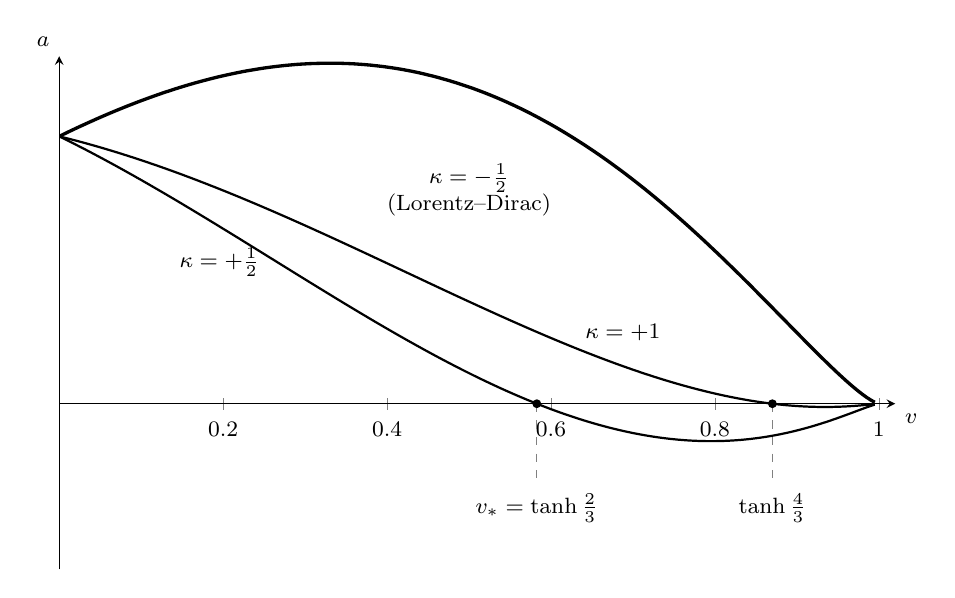
\begin{tikzpicture}
\begin{axis}[
  width=12.2cm, height=8.1cm,
  xlabel={$v$}, ylabel={$a$},
  xmin=0, xmax=1.02, ymin=-0.62, ymax=1.30,
  axis lines=middle,
  xtick={0.2,0.4,0.6,0.8,1.0},
  xticklabel style={anchor=north,yshift=-1pt},
  ytick=\empty,
  every axis y label/.style={at={(ticklabel* cs:1.0)},anchor=south east},
  every axis x label/.style={at={(ticklabel* cs:1.0)},anchor=north west},
  clip=true, samples=200, font=\footnotesize,
]

  %% drop lines marking the two equilibria, drawn first so the curves sit on top
  \draw[gray,dashed] (axis cs:0.5827,0) -- (axis cs:0.5827,-0.30);
  \draw[gray,dashed] (axis cs:0.8701,0) -- (axis cs:0.8701,-0.30);
  \node[anchor=north,font=\footnotesize] at (axis cs:0.5827,-0.30)
       {$v_*=\tanh\tfrac23$};
  \node[anchor=north,font=\footnotesize] at (axis cs:0.8701,-0.30)
       {$\tanh\tfrac43$};

  %% kappa < 0 : the Lorentz-Dirac value. a stays above the axis.
  \addplot[very thick,domain=0:0.995]
      {( 0.75*ln((1+x)/(1-x)) + 1 ) * (1-x^2)^(3/2)};
  \node[align=center,font=\footnotesize] at (axis cs:0.50,0.80)
       {$\kappa=-\tfrac12$\\(Lorentz--Dirac)};

  %% kappa > 0 : crosses the axis and returns to it
  \addplot[thick,domain=0:0.995]
      {( -0.375*ln((1+x)/(1-x)) + 1 ) * (1-x^2)^(3/2)};
  \node[anchor=south west,font=\footnotesize] at (axis cs:0.63,0.20)
       {$\kappa=+1$};

  \addplot[thick,domain=0:0.995]
      {( -0.75*ln((1+x)/(1-x)) + 1 ) * (1-x^2)^(3/2)};
  \node[anchor=south west,font=\footnotesize] at (axis cs:0.135,0.44)
       {$\kappa=+\tfrac12$};

  %% the equilibria themselves
  \fill (axis cs:0.5827,0) circle (1.6pt);
  \fill (axis cs:0.8701,0) circle (1.6pt);

\end{axis}
\end{tikzpicture}
\caption{The phase portrait of branch (a), Eq.~(\ref{eq:phase}), for $C=1$. The sign of $\kappa$ decides everything. For $\kappa<0$,
which includes the Lorentz--Dirac value $\kappa=-\tfrac12$, the bracket grows
with $v$ and the curve never returns to the axis: the acceleration is positive
at every speed, so nothing stops the particle short of $c$, and this is the
runaway of Sec.~\ref{sec:freesol} seen in the $(v,a)$ plane. For $\kappa>0$ the
bracket decreases, the curve must cross the axis, and the crossing at
$v_*=\tanh(4\kappa C/3)$ is an attractor: below it the acceleration is positive
and above it negative, so a particle released anywhere returns to $v_*$. The
terminal speed is then fixed by $C$, which is fixed by the applied impulse ---
force determines velocity rather than acceleration, which is why
\citet{zhang2006} calls this Aristotle motion. Only $v>0$ is shown; the
portrait is symmetric under $(v,a,C)\to(-v,-a,-C)$.
\label{fig:phase}}
\end{figure}
.
%% Needs pgfplots, loaded in the main preamble.
%%
%% Plots a(v) = [ -(3/8k) ln((1+v)/(1-v)) + C ] (1-v^2)^{3/2}, the closed-form
%% phase portrait of branch (a). Nothing here is drawn by hand: the zeros
%% marked on the v axis are v* = tanh(4 k C / 3), which follows from setting
%% the bracket to zero, and for the two curves shown they are
%%
%%   k = 1/2, C = 1  ->  v* = tanh(2/3)  = 0.5827
%%   k = 1,   C = 1  ->  v* = tanh(4/3)  = 0.8701
%%
%% Only v > 0 is drawn; the portrait is symmetric under (v,a,C) -> (-v,-a,-C).

\begin{figure}[htb]
\centering
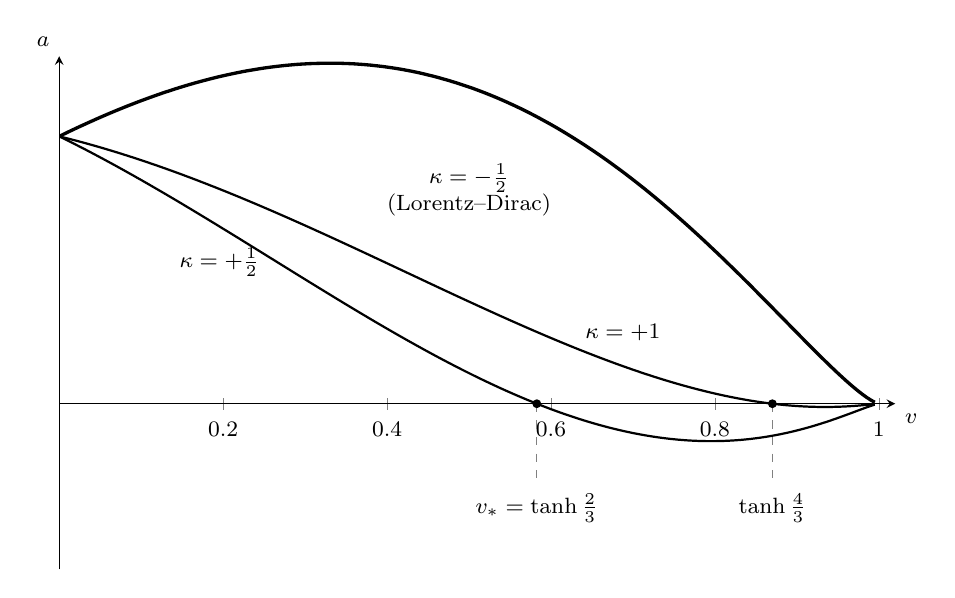
\begin{tikzpicture}
\begin{axis}[
  width=12.2cm, height=8.1cm,
  xlabel={$v$}, ylabel={$a$},
  xmin=0, xmax=1.02, ymin=-0.62, ymax=1.30,
  axis lines=middle,
  xtick={0.2,0.4,0.6,0.8,1.0},
  xticklabel style={anchor=north,yshift=-1pt},
  ytick=\empty,
  every axis y label/.style={at={(ticklabel* cs:1.0)},anchor=south east},
  every axis x label/.style={at={(ticklabel* cs:1.0)},anchor=north west},
  clip=true, samples=200, font=\footnotesize,
]

  %% drop lines marking the two equilibria, drawn first so the curves sit on top
  \draw[gray,dashed] (axis cs:0.5827,0) -- (axis cs:0.5827,-0.30);
  \draw[gray,dashed] (axis cs:0.8701,0) -- (axis cs:0.8701,-0.30);
  \node[anchor=north,font=\footnotesize] at (axis cs:0.5827,-0.30)
       {$v_*=\tanh\tfrac23$};
  \node[anchor=north,font=\footnotesize] at (axis cs:0.8701,-0.30)
       {$\tanh\tfrac43$};

  %% kappa < 0 : the Lorentz-Dirac value. a stays above the axis.
  \addplot[very thick,domain=0:0.995]
      {( 0.75*ln((1+x)/(1-x)) + 1 ) * (1-x^2)^(3/2)};
  \node[align=center,font=\footnotesize] at (axis cs:0.50,0.80)
       {$\kappa=-\tfrac12$\\(Lorentz--Dirac)};

  %% kappa > 0 : crosses the axis and returns to it
  \addplot[thick,domain=0:0.995]
      {( -0.375*ln((1+x)/(1-x)) + 1 ) * (1-x^2)^(3/2)};
  \node[anchor=south west,font=\footnotesize] at (axis cs:0.63,0.20)
       {$\kappa=+1$};

  \addplot[thick,domain=0:0.995]
      {( -0.75*ln((1+x)/(1-x)) + 1 ) * (1-x^2)^(3/2)};
  \node[anchor=south west,font=\footnotesize] at (axis cs:0.135,0.44)
       {$\kappa=+\tfrac12$};

  %% the equilibria themselves
  \fill (axis cs:0.5827,0) circle (1.6pt);
  \fill (axis cs:0.8701,0) circle (1.6pt);

\end{axis}
\end{tikzpicture}
\caption{The phase portrait of branch (a), Eq.~(\ref{eq:phase}), for $C=1$. The sign of $\kappa$ decides everything. For $\kappa<0$,
which includes the Lorentz--Dirac value $\kappa=-\tfrac12$, the bracket grows
with $v$ and the curve never returns to the axis: the acceleration is positive
at every speed, so nothing stops the particle short of $c$, and this is the
runaway of Sec.~\ref{sec:freesol} seen in the $(v,a)$ plane. For $\kappa>0$ the
bracket decreases, the curve must cross the axis, and the crossing at
$v_*=\tanh(4\kappa C/3)$ is an attractor: below it the acceleration is positive
and above it negative, so a particle released anywhere returns to $v_*$. The
terminal speed is then fixed by $C$, which is fixed by the applied impulse ---
force determines velocity rather than acceleration, which is why
\citet{zhang2006} calls this Aristotle motion. Only $v>0$ is shown; the
portrait is symmetric under $(v,a,C)\to(-v,-a,-C)$.
\label{fig:phase}}
\end{figure}
.
%% Needs pgfplots, loaded in the main preamble.
%%
%% Plots a(v) = [ -(3/8k) ln((1+v)/(1-v)) + C ] (1-v^2)^{3/2}, the closed-form
%% phase portrait of branch (a). Nothing here is drawn by hand: the zeros
%% marked on the v axis are v* = tanh(4 k C / 3), which follows from setting
%% the bracket to zero, and for the two curves shown they are
%%
%%   k = 1/2, C = 1  ->  v* = tanh(2/3)  = 0.5827
%%   k = 1,   C = 1  ->  v* = tanh(4/3)  = 0.8701
%%
%% Only v > 0 is drawn; the portrait is symmetric under (v,a,C) -> (-v,-a,-C).

\begin{figure}[htb]
\centering
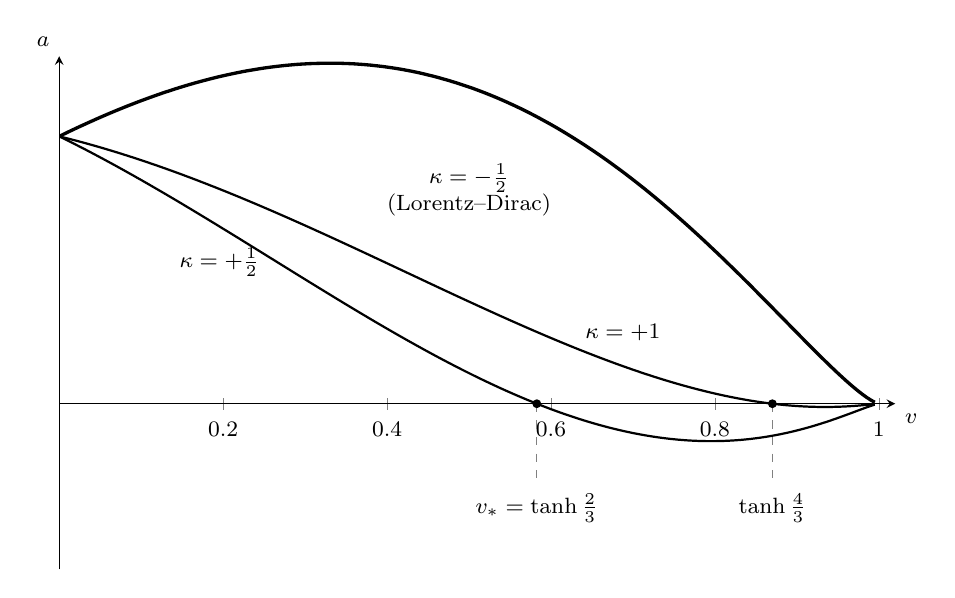
\begin{tikzpicture}
\begin{axis}[
  width=12.2cm, height=8.1cm,
  xlabel={$v$}, ylabel={$a$},
  xmin=0, xmax=1.02, ymin=-0.62, ymax=1.30,
  axis lines=middle,
  xtick={0.2,0.4,0.6,0.8,1.0},
  xticklabel style={anchor=north,yshift=-1pt},
  ytick=\empty,
  every axis y label/.style={at={(ticklabel* cs:1.0)},anchor=south east},
  every axis x label/.style={at={(ticklabel* cs:1.0)},anchor=north west},
  clip=true, samples=200, font=\footnotesize,
]

  %% drop lines marking the two equilibria, drawn first so the curves sit on top
  \draw[gray,dashed] (axis cs:0.5827,0) -- (axis cs:0.5827,-0.30);
  \draw[gray,dashed] (axis cs:0.8701,0) -- (axis cs:0.8701,-0.30);
  \node[anchor=north,font=\footnotesize] at (axis cs:0.5827,-0.30)
       {$v_*=\tanh\tfrac23$};
  \node[anchor=north,font=\footnotesize] at (axis cs:0.8701,-0.30)
       {$\tanh\tfrac43$};

  %% kappa < 0 : the Lorentz-Dirac value. a stays above the axis.
  \addplot[very thick,domain=0:0.995]
      {( 0.75*ln((1+x)/(1-x)) + 1 ) * (1-x^2)^(3/2)};
  \node[align=center,font=\footnotesize] at (axis cs:0.50,0.80)
       {$\kappa=-\tfrac12$\\(Lorentz--Dirac)};

  %% kappa > 0 : crosses the axis and returns to it
  \addplot[thick,domain=0:0.995]
      {( -0.375*ln((1+x)/(1-x)) + 1 ) * (1-x^2)^(3/2)};
  \node[anchor=south west,font=\footnotesize] at (axis cs:0.63,0.20)
       {$\kappa=+1$};

  \addplot[thick,domain=0:0.995]
      {( -0.75*ln((1+x)/(1-x)) + 1 ) * (1-x^2)^(3/2)};
  \node[anchor=south west,font=\footnotesize] at (axis cs:0.135,0.44)
       {$\kappa=+\tfrac12$};

  %% the equilibria themselves
  \fill (axis cs:0.5827,0) circle (1.6pt);
  \fill (axis cs:0.8701,0) circle (1.6pt);

\end{axis}
\end{tikzpicture}
\caption{The phase portrait of branch (a), Eq.~(\ref{eq:phase}), for $C=1$. The sign of $\kappa$ decides everything. For $\kappa<0$,
which includes the Lorentz--Dirac value $\kappa=-\tfrac12$, the bracket grows
with $v$ and the curve never returns to the axis: the acceleration is positive
at every speed, so nothing stops the particle short of $c$, and this is the
runaway of Sec.~\ref{sec:freesol} seen in the $(v,a)$ plane. For $\kappa>0$ the
bracket decreases, the curve must cross the axis, and the crossing at
$v_*=\tanh(4\kappa C/3)$ is an attractor: below it the acceleration is positive
and above it negative, so a particle released anywhere returns to $v_*$. The
terminal speed is then fixed by $C$, which is fixed by the applied impulse ---
force determines velocity rather than acceleration, which is why
\citet{zhang2006} calls this Aristotle motion. Only $v>0$ is shown; the
portrait is symmetric under $(v,a,C)\to(-v,-a,-C)$.
\label{fig:phase}}
\end{figure}


Section~\ref{sec:lkfam} already established what this branch is: the
Lorentz--Dirac equation with its reaction coefficient rescaled by $-2\kappa$,
\begin{equation}
ma^\alpha = \Fext - \frac{4\kappa}{3}e^2
\left(\dot a^\alpha - a^\beta a_\beta\,u^\alpha\right),
\label{eq:151}
\end{equation}
with $\kappa=-\tfrac12$ returning Eq.~(\ref{eq:LD}). What remains is to find out
what the rescaling does, and for the free particle in one dimension that can be
answered in closed form.

Write $a = \dot v = p(v)$, so that $\ddot v = p\,dp/dv$ and the equation of
motion becomes first order in the $(v,a)$ plane. With no external force
Eq.~(\ref{eq:151}) reduces to
\begin{equation}
\frac{dp}{dv} + \frac{3v}{1-v^2}\,p
= -\frac{3}{4\kappa}\sqrt{1-v^2},
\label{eq:phaseode}
\end{equation}
a linear equation whose integrating factor is $(1-v^2)^{-3/2}$, and which
therefore integrates at once to
\begin{equation}
a = \left[-\frac{3}{8\kappa}\ln\frac{1+v}{1-v} + C\right](1-v^2)^{3/2}.
\label{eq:phase}
\end{equation}
This is Eq.~(1.2.26) of \citet{zhang2006}. The constant $C$ is fixed by the
state the particle is put in --- for a particle kicked from rest, by the size
of the kick --- and $\kappa$ is the parameter of the family. Everything about
this branch can be read off the one curve, and it is drawn in
Fig.~\ref{fig:phase}.

The sign of $\kappa$ decides the whole question, and it decides it by
elementary means. As $v$ runs from $0$ to $1$ the logarithm runs from $0$ to
$+\infty$. So for $\kappa<0$ the bracket \emph{increases} without bound, the
curve stays above the axis at every speed, and the acceleration is positive
everywhere: nothing brings the particle to rest relative to its own motion and
it proceeds to $c$. That is the runaway of Sec.~\ref{sec:freesol}, and since
$\kappa=-\tfrac12$ lies in this range it is also the statement that
Eq.~(\ref{eq:LD}) belongs to the bad half of the family.

For $\kappa>0$ the bracket \emph{decreases}, from $C$ at $v=0$ towards
$-\infty$. It must therefore vanish somewhere, and where it vanishes the
acceleration does too. Setting the bracket to zero and using
$\ln\frac{1+v}{1-v} = 2\,\mathrm{artanh}\,v$,
\begin{equation}
v_* = \tanh\!\left(\frac{4\kappa C}{3}\right).
\label{eq:vstar}
\end{equation}
Below $v_*$ the acceleration is positive and above it negative, so $v_*$ is not
merely a zero but an attractor: a particle released at any speed is carried to
it. \citet{zhang2006} identifies the crossing and reads it as the point of
re-equilibration; Eq.~(\ref{eq:vstar}) writes it out.

That is a genuine damping. A particle disturbed from uniform motion settles
back to uniform motion, which is what criterion~\ref{crit:stability} of
Sec.~\ref{sec:criteria} asks for and what nothing in
Secs.~\ref{sec:LDdisc} or \ref{sec:eliezer} delivers.

It also has a peculiar character, and the 2006 text's name for it is the right
one. The speed the particle ends at is set by $C$, and $C$ is set by the force
that was applied. \emph{The force determines the velocity, not the
acceleration.} That is Aristotle's picture of motion rather than Newton's, and
Eq.~(\ref{eq:vstar}) is its quantitative form; hence \emph{Aristotle motion}.
It is worth being clear that this is not a slip. It is what a damping term of
this sign does: the reaction opposes the motion at every speed until the
opposition balances the applied force, exactly as a body in a viscous medium
reaches a terminal velocity, and Aristotle's mistake was to suppose that the
world is always in that regime.

Two things should be entered against this branch before it is left.

The first is that $\kappa$ is not determined. It is a free parameter, and the
theory says only that it must be positive for the behaviour above. The 2006
text is explicit that it would have to be fixed by experiment, which is what
its Sec.~5 is about and is not covered in these notes.

The second is more serious. It is not raised in the 2006 text, but it was
raised in 1947, in one sentence, by \citet{eliezer1947}: in the notation of his
Eq.~(61) a negative $2k+1$ turns what corresponds to self-acceleration into
self-retardation, and \emph{what corresponds to emission of radiation into
absorption of radiation}. Turning $\kappa$ positive reverses the sign of the
reaction term in Eq.~(\ref{eq:151}). The term whose sign was reversed is the one identified in
Sec.~\ref{sec:LDeq} as the radiated four-momentum, $-P_{\rm rad}u^\alpha/c^2$
with $P_{\rm rad}\ge0$ by the Larmor formula. Reversing it does not merely damp
the motion; it turns radiative loss into radiative gain, and
criterion~\ref{crit:conservation} of Sec.~\ref{sec:criteria} was written down
with exactly this kind of move in mind. No energy budget for
Eq.~(\ref{eq:151}) appears anywhere in the 2006 text, and it should be computed
before the $\kappa>0$ branch is taken to have solved anything. The runaway is
certainly gone. Where the energy comes from is an open question.

\subsection{Branch (b), and what the family amounts to}
\label{sec:lk-summary}
\label{sec:branchB}

Branch (b) can be dealt with quickly, because nothing later depends on it.
Setting $\lambda = 1+\kappa$ leaves the retained field with a singular part, so
the rescaling argument of Eq.~(\ref{eq:branchArescale}) does not apply and there
is no closed-form portrait; \citet{zhang2006} reduces the equation of motion and
integrates it numerically with $\kappa$ as the parameter. The result is one
watershed and two regimes. For $\kappa > -1$, of either sign, the phase curve is
convex and the electron self-accelerates much as under Eq.~(\ref{eq:LD}); larger
$\kappa$ merely lowers the acceleration without changing its sign. At
$\kappa=-1$ the portrait changes character. For $\kappa < -1$ a critical
velocity $v_c$ appears, and it is a different object from the attractor of
Sec.~\ref{sec:branchA}: a particle starting below $v_c$ remains below it for
ever, approaching it asymptotically, while one starting above it decelerates
stably.

\begin{table}[htb]
\centering
\begin{tabular}{lccccc}
\toprule
$\kappa$ & $-1.5$ & $-2$ & $-3$ & $-500$ & $-5000$ \\
\midrule
$v_c$ & $0.3473$ & $0.2261$ & $0.1341$ & $6.67\times10^{-3}$
      & $6.67\times10^{-4}$ \\
\bottomrule
\end{tabular}
\caption{The critical velocity of branch (b), from \citet{zhang2006}. The two
largest values give $|\kappa|\,v_c = 3.34$ apiece, so $v_c$ falls off as
$1/|\kappa|$ once $|\kappa|$ is large.
\label{tab:vcrit}}
\end{table}

One obstruction should be recorded, since it is the reason this branch is not
worth pursuing further as it stands. Taking it beyond one dimension requires
$\mathbf n\cdot\mathbf v$ at the position of the charge itself, where
$\mathbf n$ is not defined. \citet{zhang2006} suggests replacing it by its
angular average $\tfrac13 v$ and does not carry that through. Until something
is done about it, branch (b) exists only in one dimension.

\bigskip

What the section as a whole amounts to is branch (a), and it amounts to one
sentence. Equation~(\ref{eq:151}) is Eq.~(\ref{eq:LD}) with the coefficient of
the radiation-reaction term replaced by a free parameter. Everything else ---
the two potentials, the parity argument, the two-parameter family, the
condition $\lambda+\kappa=0$ --- is scaffolding that produces that one
modification and is then dispensable.

This is worth separating carefully from the argument that motivated it.
Section~\ref{sec:doesitact} rested the case for opening the split on
Eq.~(\ref{eq:1217}), and gave reasons to doubt it: if the singular field exerts
no force, as the Detweiler--Whiting principle asserts, then there was never any
licence to relax Eq.~(\ref{eq:retadvsplit}) and the derivation collapses. But
the equation it produced does not collapse with it. Written in a form that does
not mention $\lambda$ or $\kappa$ at all,
\begin{equation}
ma^\alpha = \Fext + \zeta\,\taunought\, m
\left(\dot a^\alpha - a^\beta a_\beta\,u^\alpha\right),
\qquad \zeta = -2\kappa ,
\label{eq:zeta}
\end{equation}
with $\zeta=1$ the standard value and $\zeta=1$ alone recovering
Eq.~(\ref{eq:LD}). This is Eliezer's Eq.~(61) again, with $\zeta = 2k+1$; the
parametrization is older than the derivation given for it here. This is a one-parameter deformation of the Lorentz--Dirac
equation, and it stands on its own whatever becomes of the reasoning that
suggested it. A derivation can be wrong and still have found something.

The virtue of Eq.~(\ref{eq:zeta}) is that $\zeta$ is a number that data can
constrain, which is more than can be said for anything else in these notes. The
sign question of Sec.~\ref{sec:branchA} is now the statement that $\zeta<0$
reverses the radiated term, and the Aristotle branch is the whole half-line
$\zeta<0$. What the existing measurements have to say about $\zeta$, and how
tightly they bound it, is a separate matter and is not taken up here.

%% ===================================================================
\section{The Eliezer-Type Series}
\label{sec:eliezer}

This is the upward branch of the fork of Sec.~\ref{sec:scorecard}: keep the
coefficient of the reaction term and raise the order of the equation. The door
was left open in Sec.~\ref{sec:Bmu}, where the tube calculation was found to fix
the particle's own four-momentum only through Eq.~(\ref{eq:Bcond}), and Dirac
closed it with the simplest choice.

The fork itself is not an invention of these notes, nor of \citet{zhang2006}. It
is stated at the head of the section \citet{eliezer1947} devotes to the problem:
there are two ways to modify the Lorentz--Dirac equation, one being to keep the
field of the electron equal to its retarded field and introduce derivatives of
the velocity higher than the second, the other to abandon the purely retarded
field and work with a combination of retarded and advanced. Those are
Secs.~\ref{sec:eliezer} and \ref{sec:lk} respectively. The 2006 text pursues
both without recording that the choice between them had been posed sixty years
earlier.

One warning before anything else, since two different equations carry the same
name. What the literature calls the Eliezer, or Eliezer--Ford--O'Connell,
equation \citep{eliezer1948,ford_oconnell1991} is obtained by \emph{reducing}
the order of Eq.~(\ref{eq:LD}), is free of runaway solutions, and is a live
candidate in present-day radiation-reaction experiments. What follows is the
opposite operation, carried out on an ansatz from the earlier review
\citep{eliezer1947}. The two sit on opposite sides of the fork just described,
and reading the conclusion of this section as a verdict on the first would
invert it exactly. Below, ``the Eliezer equation'' means the second.

\subsection{The Eliezer equation}
\label{sec:eliezereq}

Return to the balance of Sec.~\ref{sec:Bmu}. Written in Eliezer's notation the
equation of motion before any choice is made is
\begin{equation}
\dot A_\mu - \frac{2}{3}e^2\left(\frac{d\dot v_\mu}{d\tau}
  + \dot v^2 v_\mu\right) = e\,v_\sigma F^{\ \sigma}_{\mu\,\rm ext},
\label{eq:eliezerbalance}
\end{equation}
where $A_\mu$ is the particle's own four-momentum, the $P_{\rm mech}^\mu$ of
Eq.~(\ref{eq:Pmech}). Taking $A_\mu = mv_\mu$ gives Eq.~(\ref{eq:LD}); taking
$A_\mu=0$ describes a particle of zero rest mass. The question is what else
$A_\mu$ may be.

Two conditions restrict it. The first is Eq.~(\ref{eq:Bcond}), $v\cdot\dot A=0$.
The second, which Sec.~\ref{sec:Bmu} did not impose, is that
$v_\lambda A_\mu - v_\mu A_\lambda$ be a perfect differential. Together they are
much stronger than either alone. Trying the obvious two-term form,
\begin{equation}
A_\mu = P v_\mu + Q\dot v_\mu ,
\label{eq:PQform}
\end{equation}
\citet{eliezer1946} showed that no choice of $P$ and $Q$ satisfies both: the
form is simply not available. The shortest admissible extension carries one more
derivative,
\begin{equation}
A_\mu = P v_\mu + Q\dot v_\mu + R\,\frac{d\dot v_\mu}{d\tau},
\label{eq:PQRform}
\end{equation}
and imposing the two conditions on it fixes
\begin{equation}
P = \text{const} - \tfrac32 R\,\dot v^2, \qquad Q = 0, \qquad R = \text{const}.
\label{eq:PQRfixed}
\end{equation}

That $Q=0$ deserves emphasis. The coefficient of $\dot v_\mu$ is not small or
negligible; it is forbidden. So the admissible $A_\mu$ is
\begin{equation}
A_\mu = m v_\mu + k\left(\frac{2}{3}\frac{d\dot v_\mu}{d\tau}
        + \dot v^2 v_\mu\right),
\label{eq:Amu}
\end{equation}
with $m$ and $k$ constants, and substituting into
Eq.~(\ref{eq:eliezerbalance}) gives the equation this section is about,
\begin{equation}
\boxed{\;m\dot v_\mu - \frac{2}{3}e^2\left(\frac{d\dot v_\mu}{d\tau}
  + \dot v^2v_\mu\right)
+ k\,\frac{d}{d\tau}\left(\frac{2}{3}\frac{d\dot v_\mu}{d\tau}
  + \dot v^2 v_\mu\right) = e\,v_\nu F_\mu^{\ \nu}\;}
\tag{E}
\label{eq:eliezereq}
\end{equation}
the Eliezer equation, and Eq.~(1.3.4) of \citet{zhang2006}.

Set beside Eq.~(\ref{eq:LD}) the difference is a single term. Everything but
the $k$ term \emph{is} the Lorentz--Dirac equation, so
Eq.~(\ref{eq:eliezereq}) reduces to it at $k=0$, and the whole of the
modification is the proper-time derivative of the quantity whose undifferentiated
form is already there. That costs one order: Eq.~(\ref{eq:LD}) is third order in
the position and Eq.~(\ref{eq:eliezereq}) is fourth. It is the smallest step
that can be taken along this branch, and Sec.~\ref{sec:eliezerfree} is what it
buys.

Two remarks about the constants, both from \citet{eliezer1947} and neither in
the 2006 text.

First, the exclusion of $\dot v_\mu$ is the same fact that
Sec.~\ref{sec:Bexpand} obtains by a different route. There the chain of
identities from $v^\mu v_\mu=-1$ was used to trade odd derivatives for lower
ones, leaving only even terms in the series; here the two conditions on $A_\mu$
kill the odd term directly. The two arguments meet at $Q=0$.

Second, and more consequential, $k$ is not free. A classical point electron has
two constants, $m$ and $e$, and no others, so either $k$ describes some further
property of the electron or it is expressible in terms of those two. Eliezer
records that he had hoped for the first, as a way of getting Planck's constant
into a classical theory, and that it did not work. Dimensionally $k$ is a mass
times a length squared, that is $e^4/m$, so
\begin{equation}
k = \sigma\,\frac{e^4}{m},
\label{eq:sigma}
\end{equation}
with $\sigma$ a pure number to be determined by experiment. The family therefore
has one free parameter and not two, which will matter in
Sec.~\ref{sec:eliezerscan}.

\subsection{The free electron, solved}
\label{sec:eliezerfree}

Take Eq.~(\ref{eq:eliezereq}) with no external field and in the
non-relativistic limit, where it reduces to a linear equation for the
three-velocity,
\begin{equation}
\frac{d^3\mathbf V}{dt^3} - 2\alpha\,\frac{d^2\mathbf V}{dt^2}
+ \beta\,\frac{d\mathbf V}{dt} = 0,
\qquad
\alpha = \frac{e^2}{2k}, \quad \beta = \frac{3m}{2k}.
\label{eq:eliezerfree}
\end{equation}
This is third order, as promised, and being linear it can be solved outright.
Setting $\mathbf W = d\mathbf V/dt$ leaves $\ddot{\mathbf W} - 2\alpha
\dot{\mathbf W} + \beta\mathbf W = 0$, with roots
\begin{equation}
\lambda_\pm = \alpha \pm \sqrt{\alpha^2-\beta}\,,
\label{eq:roots}
\end{equation}
so that
\begin{equation}
\mathbf V = \mathbf A + e^{\alpha t}\left\{
\mathbf B\,e^{+\sqrt{\alpha^2-\beta}\,t}
+ \mathbf C\,e^{-\sqrt{\alpha^2-\beta}\,t}\right\}.
\label{eq:freesolgen}
\end{equation}

Everything now depends on the signs of $\alpha$ and of $\alpha^2-\beta$, and by
Eq.~(\ref{eq:sigma}) both are controlled by the single number $\sigma$:
\begin{equation}
\alpha = \frac{m}{2\sigma e^2},
\qquad
\alpha^2-\beta = \frac{m^2}{4\sigma^2 e^4}\left(1-6\sigma\right).
\label{eq:sigmadeps}
\end{equation}
Four regimes follow, and they exhaust the possibilities.

\begin{enumerate}

\item \textbf{$\sigma<0$.} Then $\alpha<0$ while $1-6\sigma>1$, so
$\sqrt{\alpha^2-\beta}>|\alpha|$ and the two roots straddle zero,
$\lambda_+>0>\lambda_-$. If $\mathbf B\neq0$ the motion is self-accelerating.
If $\mathbf B=0$ and $\mathbf C\neq0$ it is \emph{self-retarding}: any initial
acceleration dies away and the velocity tends to a finite constant. If both
vanish the motion is uniform. This is the only regime in which a physically
acceptable non-trivial free motion exists.

\item \textbf{$0<\sigma<\tfrac16$.} Now $\alpha>0$ and
$0<\sqrt{\alpha^2-\beta}<\alpha$, so both roots are positive. Any non-zero
$\mathbf B$ or $\mathbf C$ runs away, and the only physical solution is uniform
motion.

\item \textbf{$\sigma=\tfrac16$.} The roots coincide and
$\mathbf V = \mathbf A + e^{\alpha t}(\mathbf Bt+\mathbf C)$, with $\alpha>0$;
again both constants must vanish.

\item \textbf{$\sigma>\tfrac16$.} Here $\alpha^2<\beta$, the roots are complex,
and
\begin{equation}
\mathbf V = \mathbf A + e^{\alpha t}\left\{
\mathbf B\cos\!\big[\sqrt{\beta-\alpha^2}\,t\big]
+ \mathbf C\sin\!\big[\sqrt{\beta-\alpha^2}\,t\big]\right\}.
\label{eq:oscillating}
\end{equation}
Since $\alpha>0$ this is an oscillation whose amplitude grows without bound.
Eliezer's comment is that such a motion is quite foreign to classical theory
and cannot be compared with the wave packets of the quantum theory either.

\end{enumerate}

So the free electron already settles most of the question, analytically and in
1947. Only $\sigma<0$ admits a non-trivial acceptable motion, and even there it
requires $\mathbf B=0$, which is a condition on initial data of exactly the kind
Sec.~\ref{sec:freesol} objected to in Eq.~(\ref{eq:LD}). Raising the order has
not removed the need to impose something by hand; it has added a second
constant to impose it on.

\subsection{The electron struck by a pulse, solved}
\label{sec:eliezerpulse}

The impulse problem of Sec.~\ref{sec:freesol} can be done in the same closed
form. With a pulse of electric field $\epsilon\,\delta(t)$,
\begin{equation}
\frac{d^3v}{dt^3} - 2\alpha\frac{d^2v}{dt^2} + \beta\frac{dv}{dt}
= \gamma\,\delta(t),
\qquad \gamma = \frac{3e\epsilon}{2k},
\label{eq:eliezerpulse}
\end{equation}
and for $\sigma<0$, writing $s=\sqrt{\alpha^2-\beta}$, the solution that stays
finite at both ends is
\begin{equation}
v =
\begin{cases}
\dfrac{\gamma}{2\beta}\left(1-\dfrac{\alpha}{s}\right)
e^{(\alpha+s)t}, & t<0,\\[10pt]
\dfrac{\gamma}{\beta}\left[1-\dfrac12\left(1+\dfrac{\alpha}{s}\right)
e^{(\alpha-s)t}\right], & t>0.
\end{cases}
\label{eq:pulsesol}
\end{equation}
The two branches agree at $t=0$, and the exponents have the signs found in
Sec.~\ref{sec:eliezerfree}, so $v\to0$ as $t\to-\infty$ and
$v\to\gamma/\beta$ as $t\to+\infty$.

That limit is worth evaluating. From Eq.~(\ref{eq:eliezerpulse}),
\begin{equation}
\frac{\gamma}{\beta} = \frac{3e\epsilon}{2k}\cdot\frac{2k}{3m}
= \frac{e\epsilon}{m},
\label{eq:finalv}
\end{equation}
which is exactly the velocity a free Newtonian particle of mass $m$ acquires
from the same impulse. The equation delivers the right answer at late times,
and $k$ has dropped out of it entirely.

What $k$ controls is the approach. The electron is already moving before the
pulse arrives, on the timescale $(\alpha+s)^{-1}$, and it is still relaxing
afterwards, on the timescale $|\alpha-s|^{-1}$. Eliezer's own remark is that
this is \emph{more} symmetrical than the corresponding Lorentz--Dirac solution,
in which the electron accelerates until $t=0$ and then moves uniformly. Set
against Fig.~\ref{fig:preaccel}, this is the same trade in a different currency:
the runaway has been removed by a condition imposed at both ends, and the price
is again that the effect precedes the cause.

\subsection{An observable that was never used}
\label{sec:eliezerspectrum}

Because Eq.~(\ref{eq:pulsesol}) is explicit, so is the radiation it implies.
The rate of emission is $\tfrac23e^2(dv/dt)^2$, and Fourier resolving $dv/dt$
gives the energy radiated per unit frequency,
\begin{equation}
E_\nu = \frac{6e^4\epsilon^2}
{9\left(m-4\pi^2k\nu^2\right)^2 + 16\pi^2e^4\nu^2},
\label{eq:spectrum}
\end{equation}
against the corresponding Lorentz--Dirac result, which is
Eq.~(\ref{eq:spectrum}) with $k$ set to zero. At low frequency both reduce to
$\tfrac23e^4\epsilon^2/m^2$, the Thomson value. At high frequency they part
company: Eq.~(\ref{eq:spectrum}) falls as
$\tfrac23e^4\epsilon^2k^{-2}(2\pi\nu)^{-4}$, while the Lorentz--Dirac spectrum
falls only as $\nu^{-2}$.

This deserves to be flagged for what it is. It is a difference in a measurable
quantity --- the cross-section for scattering light off a free electron, at
frequencies high enough to matter --- between the Lorentz--Dirac equation and
its higher-order modification, available in closed form since 1947. Every
criterion in Sec.~\ref{sec:criteria} concerns the behaviour of solutions;
none of them looks at what the particle radiates. The 2006 text, which
scanned parameter space numerically for signs of unphysical motion, does not
mention Eq.~(\ref{eq:spectrum}), and neither did anything in
Secs.~\ref{sec:lorentz} to \ref{sec:lk}.

One further feature is visible in Eq.~(\ref{eq:spectrum}) and is not in
\citet{eliezer1947}. For $k>0$ the first term of the denominator vanishes at
$\nu_0 = (2\pi)^{-1}\sqrt{m/k}$, so the spectrum has a resonance there, with no
counterpart in the Lorentz--Dirac case. It is a sharp signature, and it belongs
to the sign of $k$ whose free-particle solutions Sec.~\ref{sec:eliezerfree}
has already excluded.

\subsection{The general series}
\label{sec:Bexpand}

Equation~(\ref{eq:Amu}) is the shortest admissible extension, and it is where
\citet{eliezer1947} stops: one extra derivative, one extra constant. The step
to a general series is not his. It is taken in \citet{zhang2006}, which writes
the undetermined vector as a full series in the derivatives of the
four-velocity,
\begin{equation}
B_\mu = P_0 v_\mu + P_1\dot v_\mu + P_2\ddot v_\mu + \cdots
      + P_i v^{(i)}_\mu + \cdots ,
\label{eq:Bseries}
\end{equation}
and asking which terms survive. The instrument is the normalization again.
Differentiating $v^\mu v_\mu=-1$ repeatedly gives a chain,
\begin{align}
v_\mu \dot v^\mu &= 0, \nonumber\\
v_\mu \ddot v^\mu + \dot v_\mu \dot v^\mu &= 0, \nonumber\\
v_\mu \dddot v^\mu + 3\dot v_\mu \ddot v^\mu &= 0, \nonumber\\
v_\mu v^{(4)\mu} + 4\dot v_\mu \dddot v^\mu + 3\ddot v_\mu \ddot v^\mu &= 0,
\nonumber\\
v_\mu v^{(5)\mu} + 5\dot v_\mu v^{(4)\mu} + 10\ddot v_\mu \dddot v^\mu &= 0,
\label{eq:vchain}
\end{align}
whose coefficients are those of Pascal's triangle, the identities coming from
the Leibniz rule; the general term is Appendix A.4 of \citet{zhang2006}. Each
identity lets an odd-order derivative of $v_\mu$ be traded for lower ones, so
the odd terms of Eq.~(\ref{eq:Bseries}) are not independent, and what remains is
\begin{equation}
B_\mu = \Big\{k - \tfrac32 P_2(\dot v)^2
  - 5P_4\,\dot v_\mu \dddot v^\mu - \tfrac52 P_4(\ddot v)^2 - \cdots\Big\}v_\mu
  \;+\; P_2\ddot v_\mu + P_4 v^{(4)}_\mu + \cdots + P_{2i}v^{(2i)}_\mu ,
\label{eq:Bgeneralform}
\end{equation}
Eq.~(1.3.2) of \citet{zhang2006}, with one undetermined constant for each even
derivative retained.

The relation to Sec.~\ref{sec:eliezereq} is worth stating precisely, since the
two arguments are easily confused. Eliezer's conditions kill the $\dot v_\mu$
term once, at the first step, and stop there; the identity chain kills every odd
term at every order, and so extends the same conclusion to the whole series.
Truncating Eq.~(\ref{eq:Bgeneralform}) after $P_2$ returns
Eq.~(\ref{eq:Amu}), and setting every $P_{2i}$ to zero returns
Eq.~(\ref{eq:LD}).

What Eq.~(\ref{eq:sigma}) said about $k$ applies at every order and gets worse.
Each retained $P_{2i}$ is a further constant that the theory does not fix and
that no measurement has been proposed to fix, and it arrives together with two
more orders of derivative.

\subsection{The relativistic equation and the 2006 scans}
\label{sec:eliezerscan}

The 2006 text works relativistically and numerically rather than
non-relativistically and analytically. Reducing Eq.~(\ref{eq:eliezereq}) to one
dimension with the rapidity of Sec.~\ref{sec:1dreduction} gives
\begin{equation}
\dddot q - B\ddot q + A\dot q - \tfrac12 \dot q^{\,3} = 0,
\qquad
A = \frac{3m}{2k}, \quad B = \frac{e^2}{k},
\label{eq:third}
\end{equation}
which is Eq.~(\ref{eq:eliezerfree}) with $A=\beta$, $B=2\alpha$, plus the
relativistic term $-\tfrac12\dot q^{\,3}$. The parameters therefore carry the
constraints already found: $A$ and $B$ have the same sign, since both are
divided by $k$, and their ratio is fixed,
\begin{equation}
\frac{B}{A} = \frac{2e^2}{3m} = \taunought
\label{eq:BoverA}
\end{equation}
in units with $c=1$. There is one free number, $\sigma$, exactly as
Eq.~(\ref{eq:sigma}) says.

The scan reported in \citet{zhang2006} finds that for every sampled $(A,B)$ the
electron accelerates itself to $c$: monotonically for $A,B<0$, much as under
Eq.~(\ref{eq:LD}), and for $A,B>0$ with $A\gg B$ by swinging between $+c$ and
$-c$ at large amplitude and high frequency. Figures 1-3-1 to 1-3-4 there show
$v(\tau)$ for $(A,B)=(2,1)$, $(3,1)$, $(10,1)$ and $(100,1)$.

Those results are not independent of Sec.~\ref{sec:eliezerfree}. The oscillatory
regime of Eq.~(\ref{eq:oscillating}) is $\alpha^2<\beta$, which in the present
variables reads
\begin{equation}
A > \frac{B^2}{4},
\label{eq:osccondition}
\end{equation}
and all four sampled pairs satisfy it. The violent swinging between $\pm c$ is
the relativistic form of the growing oscillation Eliezer wrote down in closed
form in 1947, with the relativistic term supplying the bound at $\pm c$ that the
linear equation lacks. The numerical scan rediscovered an analytic result rather
than establishing a new one, and reading the two together sharpens both.

Retaining $P_4$ as well produces a fifth-order equation, Eq.~(1.3.11) of
\citet{zhang2006},
%% CHECK: transcribed from the scanned Eq. (1.3.11); the coefficients 25/2,
%% 3/2 and 1/2 should be verified against the original.
\begin{equation}
q^{(5)} + \left[C + 5\dot q^{\,2}\right]\dddot q
 - B\ddot q
 + \left[A + \tfrac{25}{2}\dot q^{\,2}\right]\dot q
 - \tfrac32 \dot q^{\,5}
 - \tfrac12 C \dot q^{\,3} = 0 ,
\label{eq:fifth}
\end{equation}
with $C=P_2/P_4$, whose sign is free where those of $A$ and $B$ are not. The
scan of twenty-two triples, from rest with $q^{(4)}(0)=2$, produces three
classes of behaviour.

\begin{table}[htb]
\centering
\begin{tabular}{ll}
\toprule
Behaviour & Sampled $(A,B,C)$ \\
\midrule
Oscillation between $\pm c$
  & $(100,1,1)$, $(100,1,-1)$, $(100,1,-100)$, $(1000,1,-1000)$, \\
  & $(-1,-100,100)$ \\[2pt]
Monotonic approach to $c$, as under LD
  & $(-100,-1,1)$, $(-100,-1,100)$, $(-100,-1,-10)$, \\
  & $(-1000,-1,-1000)$ \\[2pt]
Neither: bounded periodic pulsation
  & $(100,1,100)$, $(100,1,1000)$, $(1000,1,100)$, \\
  & $(1000,1,1000)$, $(10000,1,1000)$, $(-1,-100,1)$, \\
  & $(-1,-1000,10)$ \\
\bottomrule
\end{tabular}
\caption{The fifth-order scan of \citet{zhang2006}, grouped by outcome rather
than in its original order. The original table lists $(100,1,1)$ twice with
contradictory verdicts and repeats three further triples; one of each is kept
here, and the class boundaries should be redone before any weight is put on
them.
\label{tab:fifthscan}}
\end{table}

The first two classes are the ones already met. The third is not: the electron
neither reaches $c$ nor returns to uniform motion, but settles into a periodic
pulsation of the speed within a bounded range --- in the 2006 text's phrase,
very like an oscillator, except that the oscillator itself keeps moving forward.
This is the case criterion~\ref{crit:stability} of Sec.~\ref{sec:criteria} was
written to admit, and it is the one thing in this section that the third-order
equation, and hence Eliezer's analysis, does not contain.

\subsection{What the branch was worth}
\label{sec:eliezerscore}

Against Sec.~\ref{sec:criteria}: criterion~\ref{crit:ivp} degrades at every
step, each retained $P_{2i}$ adding two orders and two more constants that no
measurement supplies; criterion~\ref{crit:stability} fails at third order for
every $\sigma$ except the negative ones, and there only if a constant is set to
zero by hand, and is met by part of the fifth-order parameter space;
criterion~\ref{crit:conservation} is never tested at all.

There is also a contemporary verdict that the 2006 text does not engage.
\citet{plass1961}, reviewing the whole subject, held that the standard
objections to the Lorentz--Dirac equation were largely invalid, that the extra
constants of integration are fixed by requiring that the particle not gain more
energy over long times than the external forces supply, and that on that
prescription a physical solution exists in every case examined --- including,
by numerical integration, attractive and repulsive Coulomb fields, where he
found no evidence of divergent or unstable solutions. On Eliezer specifically
he objected that demonstrating the existence of divergent solutions proves
nothing, since divergent solutions always exist, and that a non-divergent
physical solution exists for each set of initial conditions. Whether or not one
accepts that, it is the position the case for modifying Eq.~(\ref{eq:LD}) has
to answer, and neither \citet{eliezer1947} nor \citet{zhang2006} answers it.

There is also a sense in which nothing in this section is a finished theory,
and it is worth naming precisely, because it is not the usual complaint about
higher derivatives.

At Eliezer's order the equation carries one constant, $k$, that the theory does
not determine. He is candid about having wanted it to determine something --- to
be a place where Planck's constant might enter a classical theory --- and about
that not having worked, so that $k$ has to be written as $\sigma e^4/m$ with
$\sigma$ left to experiment. One undetermined number is a tolerable state of
affairs; it is what Eq.~(\ref{eq:zeta}) also amounts to, and numbers left to
experiment can be measured.

The general series is a different matter. Every retained $P_{2i}$ in
Eq.~(\ref{eq:Bgeneralform}) is another constant, the theory fixes none of them,
no measurement has been proposed for any of them, and there is no principle in
sight that would say where to truncate. What Eq.~(\ref{eq:Bseries}) defines is
therefore not an equation of motion but a family of them indexed by an infinite
sequence of unknowns --- a parametrization rather than a theory. That is the
respect in which the branch is incomplete, and it is incomplete by construction
rather than by oversight: the two conditions on $A_\mu$ constrain the series
without ever closing it.

What the branch was worth, then, is this. It produced one class of solution not
available at lower order, and one observable prediction,
Eq.~(\ref{eq:spectrum}), that nobody has used. It cost a free constant and two
orders per step, it did not remove the need to impose a condition by hand, and
it never closed.
And the question the 2006 text closed on ---

\begin{quote}
Would nature really go and choose a more complicated $B_\mu$? And if it did, we
truly cannot imagine the source of nature making such a choice.
\end{quote}

--- has since been answered, though not in a way available in 2006. That answer
belongs with the other twenty-years-on material and is not taken up here.

%% ===================================================================
\section{Twenty Years On}
\label{sec:twentyyears}

This section pays the debts the previous five deliberately left standing.
Section~\ref{sec:scorecard} set up the fork and declined to say which branch
survives. Sections~\ref{sec:lk} and \ref{sec:eliezer} each followed one branch
on its own terms, and each closed by saying that the verdict was not available
in 2006. It is available now, and so is the answer to the question
\citet{zhang2006} closed on, and so is the fate of its Sec.~5, which declared
the discriminating experiment infeasible.

\subsection{Why the runaway is not a defect of the equation}
\label{sec:verdict}

The runaway of Sec.~\ref{sec:freesol} is not a defect of Eq.~(\ref{eq:LD}). It
is what appears when every solution of an effective equation is read as a
possible motion, and it disappears as soon as the equation is read as the
approximation it is. That claim can be made precise using nothing beyond the
one-dimensional form already derived, and this subsection does so.

Take Eq.~(\ref{eq:LD1d}) and solve it for the highest derivative rather than
the lowest:
\begin{equation}
\taunought\,\ddot q = \dot q - \frac{f}{m}.
\label{eq:singular}
\end{equation}
The small parameter multiplies the highest derivative. That is the defining
signature of a \emph{singular} perturbation, and it carries a standard
consequence: the solutions split into a low-dimensional family on which the
motion is slow, and transverse directions on which it is fast.

The fast directions come out in two lines. Put $w=\dot q$, let $w_{\rm s}$ be
any solution, and perturb, $w = w_{\rm s}+\delta$; Eq.~(\ref{eq:singular}) then
gives $\taunought\dot\delta = \delta$, so
\begin{equation}
\delta = \delta_0\,e^{\tau/\taunought}.
\label{eq:fastmode}
\end{equation}
This is Eq.~(\ref{eq:runaway}) over again, and it has changed status. It is not
a solution that has to be forbidden; it is the unstable transverse direction of
a singularly perturbed system, and nothing physical is found on it for the
reason that nothing physical is found on any unstable direction.

The slow family is equally explicit. Ask for the motions in which $\dot q$ is
fixed by the applied force alone, and Eq.~(\ref{eq:singular}) is solved term by
term by
\begin{equation}
\dot q = \sum_{n=0}^{\infty}\taunought^{\,n}\,
\frac{d^n}{d\tau^n}\!\left(\frac{f}{m}\right)
= \frac{f}{m} + \taunought\frac{d}{d\tau}\!\left(\frac{f}{m}\right)
+ \taunought^{2}\frac{d^2}{d\tau^2}\!\left(\frac{f}{m}\right) + \cdots,
\label{eq:slowmanifold}
\end{equation}
as substituting back confirms at once. This is the slow manifold, and it
settles the question. It carries no free constant: given the force, the motion
is determined by position and velocity alone, which is the Newtonian count.
Equation~(\ref{eq:LD1d}) has state $(x,q,\dot q)$, one dimension more, and that
one extra dimension is Eq.~(\ref{eq:fastmode}). One extra dimension, one
unstable direction, one datum that Sec.~\ref{sec:freesol} had to supply by hand
--- three descriptions of the same thing.

Two complaints entered earlier can now be withdrawn in their own terms.
Section~\ref{sec:freesol} objected that $C_1=0$ is imposed without warrant; in
the present language it says that the data lie on
Eq.~(\ref{eq:slowmanifold}), which is an invariant set the equation itself
determines and not a convention. Section~\ref{sec:asymptotic}'s condition at
$\tau=\pm\infty$ was a way of locating that same set without having the concept
of it, and the pre-acceleration it introduced is the cost of the indirection
rather than a property of the motion.

None of the above is an invention of these notes. The reading of
Eq.~(\ref{eq:LD}) as a singularly perturbed system, and of its physical
solutions as a manifold rather than a selected subset, is due to
\citet{spohn2000} and is set out at length in \citet{spohn2004}. What is proved
there, for the Abraham--Lorentz model, is that the critical manifold exists,
that it is normally hyperbolic, that no solution on it runs away, and that to
first order in $\taunought$ the motion on it obeys
\begin{equation}
\dot q = \frac{f}{m} + \taunought\,\frac{d}{d\tau}\!\left(\frac{f}{m}\right),
\label{eq:LL1d}
\end{equation}
the truncation of Eq.~(\ref{eq:slowmanifold}) after the first correction. That
equation has a name and a section of its own, and the point to carry into it is
that it was not proposed as a replacement for Eq.~(\ref{eq:LD}). It is
Eq.~(\ref{eq:LD})'s own slow manifold, written down.

Where this stands now. The reading above is the standard one and is not in
dispute; the disagreements recorded in Secs.~\ref{sec:lorentz} to
\ref{sec:eliezer}, over which modification of Eq.~(\ref{eq:LD}) to adopt, are
closed, and they are closed because the premise they shared --- that the
equation needed modifying --- was abandoned. What remains active is narrower and
more technical. The series in Eq.~(\ref{eq:slowmanifold}) is asymptotic rather
than convergent, and its structure and resummation have continued to be studied,
as has the variational formulation of the equation and its extension to
post-Newtonian settings.%
%% TODO cite the 2021 transseries work and the 2025 variational and
%% post-Newtonian papers; REVIEW_2026.md lists them by year without references.
{}

\subsection{The Landau--Lifshitz equation, and why it has no free parameter}
\label{sec:LLeq}

Section~\ref{sec:verdict} produced Eq.~(\ref{eq:LL1d}) as the first truncation
of a slow manifold. Written covariantly it is
\begin{equation}
ma^\mu = F^\mu_{\rm ext}
+ \taunought\left(\delta^\mu{}_\nu + c^{-2}u^\mu u_\nu\right)
\frac{dF^\nu_{\rm ext}}{d\tau},
\label{eq:LL}
\end{equation}
the Landau--Lifshitz equation, given in \S76 of \citet{landau_lifshitz}, with
$dF/d\tau$ evaluated on the zeroth-order motion. Its provenance is worth being
exact about, because three separate results are doing the work. The equation
itself is Landau and Lifshitz's. That its solutions are the physical ones ---
that the reduction is not merely a convenient truncation --- is
\citet{spohn2000}. And that it follows from a controlled limit rather than from
a choice is \citet{gralla2009}, discussed below. It is not boxed, and the omission is the
point of Sec.~\ref{sec:verdict}: (AL), (LD) and (E) are candidate laws of
motion, and Eq.~(\ref{eq:LL}) is not a fourth candidate but a consequence of the
second.

Carrying out the differentiation makes the content visible. With
$F^\mu_{\rm ext} = (e/c)F^{\mu\nu}u_\nu$ and $\dot u_\nu = F_\nu/m$ to the order
kept,
\begin{equation}
\frac{dF^\mu_{\rm ext}}{d\tau}
= \frac{e}{c}\,\partial_\alpha F^{\mu\nu}u^\alpha u_\nu
+ \frac{e^2}{mc^2}\,F^{\mu\nu}F_{\nu\lambda}u^\lambda ,
\label{eq:Fdot}
\end{equation}
so the correction consists of one term in the gradient of the external field and
two quadratic in the field itself, the second of which is the radiated
four-momentum. No derivative of the acceleration survives anywhere:
$\dot a^\mu$ has been traded for $\dot F^\mu_{\rm ext}$, which is a property of
the applied field and is known before the motion is solved for.

That trade is what buys the good behaviour. Equation~(\ref{eq:LL}) is second
order, so it is solved from $(x,v)$ like any equation of mechanics; there is no
runaway, since Eq.~(\ref{eq:fastmode}) was the transverse direction that has
been projected out; and there is no pre-acceleration, since nothing is imposed
at $\tau\to\pm\infty$. All three criteria of Sec.~\ref{sec:criteria} are met at
once, which Sec.~\ref{sec:scorecard} showed Eq.~(\ref{eq:LD}) cannot do under
any choice of boundary condition. The price is stated plainly by
Sec.~\ref{sec:verdict}: Eq.~(\ref{eq:LL}) does not claim to be exact, and holds
to first order in $\taunought$.

\medskip

Now the count, which is the subject of this subsection.

\begin{center}
\begin{tabular}{lcc}
\toprule
Equation & Free parameters & Data beyond $(x,v)$ \\
\midrule
Lorentz--Dirac, Eq.~(\ref{eq:LD})      & $0$      & $1$ per particle \\
Eliezer, Eq.~(\ref{eq:eliezereq})      & $1$ ($\sigma$) & $2$ \\
The series, Eq.~(\ref{eq:Bseries})     & $\infty$ & grows with order \\
The $\lambda$--$\kappa$ family, Eq.~(\ref{eq:zeta}) & $1$ ($\zeta$) & $1$ \\
Landau--Lifshitz, Eq.~(\ref{eq:LL})    & $\mathbf 0$ & $\mathbf 0$ \\
\bottomrule
\end{tabular}
\end{center}

\medskip

The coefficient in Eq.~(\ref{eq:LL}) is $\taunought = 2e^2/3mc^3$, fixed by the
charge and the mass and by nothing else, and the same is true of every further
term of Eq.~(\ref{eq:slowmanifold}). This is not the usual situation in an
effective theory, where each order brings a coefficient to be measured. It
happens here because a classical point charge has nothing to renormalize beyond
its mass: once that is absorbed, as in Eq.~(\ref{eq:massren2}), the expansion is
determined.

The tower of Sec.~\ref{sec:Bexpand} therefore collapses, and it is worth being
exact about how. Different choices of $B^\mu$ correspond to adding to an
effective action terms proportional to the equation of motion, and such terms
are removed by a redefinition of the field variables, which changes no physical
prediction. So the constants $P_{2i}$ of Eq.~(\ref{eq:Bgeneralform}) are not
undetermined quantities awaiting measurement. They are a choice of coordinates,
not new structure in the point-particle theory. Section~\ref{sec:eliezerscore}
closed on the question of whether nature would choose a more complicated
$B_\mu$; in the point-charge limit the answer is that this is not an additional
choice of physics.

Two things make that a result rather than a convention. The first is
\citet{gralla2009}, who obtain the self-force from a controlled point-particle
limit --- a body of finite size scaled down along a one-parameter family of
solutions --- with no tube, no cap integrals and no undetermined four-vector.
Both reservations of Sec.~\ref{sec:reservations} are bypassed rather than
answered, since the construction that produced them is never used. The second
is Eq.~(\ref{eq:slowmanifold}) itself, which was constructed without any freedom
to choose.

One qualification. All of this is for a structureless point charge. Give the
particle structure and genuine parameters appear --- a polarizability, a form
factor --- but they describe the structure, and Sec.~\ref{sec:direct} already
showed where they live: the terms of Eq.~(\ref{eq:ALseries}) with $n\ge3$,
which the point limit destroys. They are not a radiation-reaction coefficient
under another name.

A count of zero is a strong statement, and it invites the obvious question:
if the equation has nothing to measure, what is left for an experiment to do?
Section~\ref{sec:whichequation} answers it, and the answer is not that nothing
is left.

Finally, a remark that belongs in these notes rather than in the literature. The
author's own later drafts, \texttt{2010paper.pdf} and \texttt{2011paper.pdf} in
this repository, both take Eq.~(\ref{eq:LL}) as their starting point and cite
Poisson and Rohrlich for it. The move away from the programme of
Secs.~\ref{sec:lk} and \ref{sec:eliezer} was therefore made in 2010, four years
after the text those sections reconstruct, and made without comment.

\subsection{Which equation the field uses, and why the rest cannot be told
apart}
\label{sec:whichequation}

Five sections have put nine equations on the table, and two of the nine are
families rather than single equations, one of them infinite. Before asking
where the classical description stops (Sec.~\ref{sec:classquantum}) and what
has been measured (Sec.~\ref{sec:experiment}), it is worth collecting them in
one place and saying what became of each. The answer is short, and it is not
the answer Secs.~\ref{sec:lk} and \ref{sec:eliezer} were working towards.

\subsubsection{The roster}
\label{sec:roster}

Table~\ref{tab:roster} is every equation these notes have written down.

\begin{deluxetable}{lccl}
\tablecaption{The candidates, in the order they were introduced.
\label{tab:roster}}
\tablehead{
\colhead{Equation} & \colhead{Order} & \colhead{Parameters} &
\colhead{Status in 2026}
}
\startdata
Lorentz force                              & 2 & 0        & exact when radiation is negligible \\
Abraham--Lorentz, Eq.~(\ref{eq:AL})        & 3 & 0        & teaching, non-relativistic \\
Lorentz--Dirac, Eq.~(\ref{eq:LD})          & 3 & 0        & the reference law; not a practical evolution law \\
Eliezer, Eq.~(\ref{eq:eliezereq})          & 3 & 1 ($\sigma$) & not standard \\
The $B^\mu$ series, Eq.~(\ref{eq:Bseries}) & $\ge3$ & $\infty$ & field redefinitions in the point limit \\
$\lambda$--$\kappa$ family, Eq.~(\ref{eq:zeta}) & 3 & 1 ($\zeta$) & not a viable free theory; see Sec.~\ref{sec:whycoefficient} \\
Landau--Lifshitz, Eq.~(\ref{eq:LL})        & 2 & 0        & \textbf{standard classical workhorse} \\
Eliezer--Ford--O'Connell, Eq.~(\ref{eq:third}) & 2 & 0    & alternative comparison model \\
LL with $g(\chi)$, Eq.~(\ref{eq:gaunt})    & 2 & 0        & the quantum-corrected mean \\
\enddata
\tablecomments{``Order'' is the highest derivative of position. ``Parameters''
counts numbers not fixed by $e$ and $m$. The kinetic descriptions of
Sec.~\ref{sec:classquantum} are omitted because they are not equations of
motion.}
\end{deluxetable}

The list has a shape worth noticing before any verdict is passed on it. Every
entry that is third order or higher carries either a free parameter or extra
initial data or both; both second-order entries carry neither. That is not a
coincidence, and Sec.~\ref{sec:verdict} explained it: an extra derivative is an
extra solution, and an extra solution has to be selected by something.

\subsubsection{Each candidate was removed by a different argument, and none of
them by experiment}
\label{sec:verdicts}

Four distinct arguments did the work, and it is worth keeping them separate
because they are not interchangeable.

\emph{Field redefinition.} The $B^\mu$ tower is not a set of undetermined
constants in the point-particle theory but a relabelling of what is called the
particle's position at order $\taunought$. Within that description there is no
separate observable attached to the constants $P_{2i}$. This is
Sec.~\ref{sec:LLeq}, and it removes the infinite family as a list of
independent point-charge theories.

\emph{Energy conservation.} The $\lambda$--$\kappa$ family varies the size of
the reaction term. That size is not available to be varied: the Larmor formula
follows from Maxwell's equations alone, with no equation of motion anywhere in
its derivation, and requiring that the energy the particle loses equal the
energy the field carries away fixes the coefficient. Eliezer made this objection
in 1947 and it has not been answered since.

\emph{Spurious degrees of freedom.} The higher-derivative branch of
Sec.~\ref{sec:eliezer} adds a solution at every order. The parent theory --- a
body of finite size coupled to its own field --- has position and velocity and
nothing else, so an equation requiring $\dddot q$ as initial data is asking for
information that does not exist. This is why the runaways of
Sec.~\ref{sec:freesol} are not a defect to be repaired but a signal that too
many solutions are being carried, and why the reduction of
Sec.~\ref{sec:verdict} is the cure.

\emph{Derivation.} What replaced all of it is not an argument against the
alternatives at all. \citet{gralla2009} obtain the self-force as a controlled
limit of a finite body, and what comes out is the form of Eq.~(\ref{eq:LL}).
Once the equation is derived rather than postulated there is no list to choose
from.

None of these is an experimental result. Nothing in the list was excluded by
data as a choice among classical point-particle forms, and
Sec.~\ref{sec:experiment} will show why: in the regime where that description
applies, the differences are too small to have been isolated experimentally.

\subsubsection{Landau--Lifshitz became the standard workhorse, for three reasons}
\label{sec:whyLL}

The practical answer to ``which equation'' is a single one.
Equation~(\ref{eq:LL}) is what is in the particle-in-cell codes, in the
strong-field laser modelling and in much of the pulsar-magnetosphere work, and
it is the classical limit against which quantum treatments are checked. Three
separate things put it there.

\emph{It is the only one that can be used as an ordinary initial-value law.}
Equation~(\ref{eq:LD}) needs an initial acceleration, and almost every choice of
it runs away; a numerical integration will find the runaway whether or not the
analyst wants it.
Equation~(\ref{eq:LL}) is solved from $(x,v)$ like any equation of mechanics.
This is a mundane reason and it is probably the operative one.

\emph{Inside the classical domain nothing else is distinguishable.} The
candidates differ at second order in the expansion parameter
$\epsilon = \taunought\gamma\omega_B$, and Fig.~\ref{fig:regime} fixes how
large that can get: the line $\epsilon=1$ lies a factor $3/2\alpha$ above the
line $\chi=1$, so
\begin{equation}
\epsilon\big|_{\chi=1} = \frac{2\alpha}{3} = 4.9\times10^{-3},
\qquad
\epsilon^2\big|_{\chi=1} = 2.4\times10^{-5},
\label{eq:formgap}
\end{equation}
and at $\chi=0.01$, where the quantum suppression of the radiated power is
still only $5\%$, $\epsilon^2\approx2\times10^{-9}$. So in the
whole region where the classical description is even approximately valid, the
trajectories predicted by Lorentz--Dirac, Landau--Lifshitz and
Eliezer--Ford--O'Connell agree to better than one part in $10^{5}$, and where it
is actually accurate they agree to one part in $10^{9}$. \emph{Within the
classical point-particle domain, the choice among these forms is not an
experimentally reachable question.} The disagreement between Landau--Lifshitz
and Ford--O'Connell is real, and it is located inside Eq.~(\ref{eq:formgap}).

\emph{It is derived, not selected.} This is Sec.~\ref{sec:verdicts}, and it is
the reason the first two do not feel like a compromise.

\subsubsection{The form cannot be tested, so the coefficient is what is left}
\label{sec:whycoefficient}

Equation~(\ref{eq:formgap}) has a consequence these notes have been building
towards without stating it. If the differences among the candidate \emph{forms}
are $10^{-5}$ at the very best and $10^{-9}$ in practice, then eighty years of
argument about which equation is correct has been an argument about something no
measurement has reached in the classical point-particle domain. Everything in
Secs.~\ref{sec:lorentz} to
\ref{sec:eliezer}, and everything in Table~\ref{tab:roster}, lives inside that
gap.

What does not live inside it is the coefficient. Write
\begin{equation}
ma^\alpha = \Fext + \zeta\,\taunought\,m
\left(\dot a^\alpha - a^\beta a_\beta u^\alpha\right),
\qquad \zeta = 1 \ \text{predicted},
\label{eq:zetadef}
\end{equation}
which is Eq.~(\ref{eq:zeta}) with $\zeta=-2\kappa$, reduced in order before use.
Then $\zeta$ multiplies the radiated power directly: double it and the energy
loss doubles. It is the one quantity in this problem to which an experiment is
linearly sensitive.

The distinction that matters is what $\zeta$ is for. It is not a free parameter
of any theory on the roster --- Lorentz--Dirac, Eliezer, Landau--Lifshitz and
Ford--O'Connell all predict $\zeta=1$, since all of them inherit the coefficient
from Larmor. Nor is it a revival of the $\lambda$--$\kappa$ family, which
offered a different value as an \emph{alternative} and was excluded for it in
Sec.~\ref{sec:verdicts}. It is a null-test parameter, introduced for the same
reason $\gamma$ and $\beta$ are introduced in the parameterised post-Newtonian
formalism: general relativity predicts $\gamma=1$ with no freedom whatever, and
one writes $\gamma$ anyway, in order to say how well the prediction is known.

Said that way the gap is visible. The parameters that are free --- the $P_{2i}$,
the order of the equation --- change no observable, which is why they can be
infinite in number. The parameter that changes an observable is not free. These
are not two statements but one, and the practical upshot is that the only
number in this subject that data can constrain is a number nobody has thought to
constrain, because theory fixed it and everyone believed the theory.

The state of that constraint is the subject of Sec.~\ref{sec:experiment}, and
the short version is a split: the storage rings of Sec.~\ref{sec:rings} measure
$\zeta$ and nothing else, at $\chi\sim10^{-6}$, but the literature does not
seem to quote a dedicated bound phrased this way; the strong-field experiments
of Secs.~\ref{sec:e144} to \ref{sec:los2026} measure $g(\chi)$ while
\emph{assuming} $\zeta=1$, so the joint constraint on the pair still appears to
be missing.

\subsection{When quantum electrodynamics takes over}
\label{sec:classquantum}

Everything so far has been classical, and the question of where that stops has
a sharp answer with an uncomfortable consequence: \emph{the classical theory
never reaches the field at which it would break down on its own terms.}
Quantum mechanics takes over first, and by a fixed factor.

The parameter that decides is
\begin{equation}
\chi = \frac{\gamma B_\perp}{B_S},
\qquad
B_S = \frac{m^2c^3}{e\hbar} = 4.41\times10^{13}~{\rm G},
\label{eq:chi}
\end{equation}
$B_\perp$ being the field component transverse to the motion and $B_S$ the
Schwinger field. What $\chi$ measures is the fraction of the particle's own
energy carried off by a single emitted photon. For $\chi\ll1$ the electron
loses its energy in many small pieces, which is what a continuous radiated
power describes; for $\chi\gtrsim1$ a single photon takes a sizeable part of
it, and a description in which energy leaks out smoothly is not an
approximation to that but a different thing altogether.

Three thresholds are worth separating, since they are usually run together and
they fail differently. All three run the same way: the classical description
requires the quantity to be \emph{small}, and it is exceeded by going to
stronger field or to higher energy, never the reverse. There is no lower
boundary to the classical region.

\begin{center}
\begin{tabular}{lll}
\toprule
Parameter & Classical requires & What fails once it is exceeded \\
\midrule
$\chi = \gamma B_\perp/B_S$ & $\chi\ll1$
  & photon recoil is not small, and the classical \\
 & & emission formula is wrong at leading order, \\
 & & not merely corrected \\[3pt]
$b = B/B_S$ & $B\ll4.41\times10^{13}$~G
  & Landau quantization freezes the transverse \\
 & & motion; there is no gyration left for an \\
 & & equation of motion to describe \\[3pt]
$\taunought\gamma\omega_B$ & $\gamma B\ll9.07\times10^{15}$~G
  & classical radiation reaction ceases to be \\
 & & perturbative, and $\taunought$ merges with the \\
 & & dynamical timescale \\
\bottomrule
\end{tabular}
\end{center}

%% figures/fig-regime.tex -- Figure for Sec. 6.3.
%% Pulled into notes.tex with %% figures/fig-regime.tex -- Figure for Sec. 6.3.
%% Pulled into notes.tex with %% figures/fig-regime.tex -- Figure for Sec. 6.3.
%% Pulled into notes.tex with \input{figures/fig-regime}.
%% Needs pgfplots, loaded in the main preamble.
%%
%% The (B, gamma) plane in log-log. Every boundary below is a computed number,
%% not a drawn one; the arithmetic is in the appendix of REVIEW_2026.md and
%% reproduced here:
%%
%%   B_S   = m^2 c^3 / (e hbar) = 4.414e13 G      log10 = 13.645
%%   B_cl  = m^2 c^4 / e^3      = 6.049e15 G      log10 = 15.782  ( = B_S/alpha )
%%   gamma B at tau_0 gamma omega_B = 1 : 3 m^2 c^4 / (2 e^3) = 9.073e15 G
%%                                                   log10 = 15.958
%%
%% Lines of constant gamma*B are straight with slope -1 here:
%%   chi = 0.1        log10 gamma = 12.645 - log10 B
%%   chi = 1          log10 gamma = 13.645 - log10 B
%%   tau_0 g w_B = 1  log10 gamma = 15.958 - log10 B
%% The last two are separated by a factor 3/(2 alpha) = 205.6, i.e. 2.31 decades.
%%
%% Laser point: a0 = 10 at 800 nm gives a lab field 1.34e9 G; head-on the
%% electron sees 2E = 2.68e9 G (log10 = 9.428), so with gamma = 1500
%% (log10 = 3.176) this is chi = 2 gamma E / B_S = 0.091.

\begin{figure}[htb]
\centering
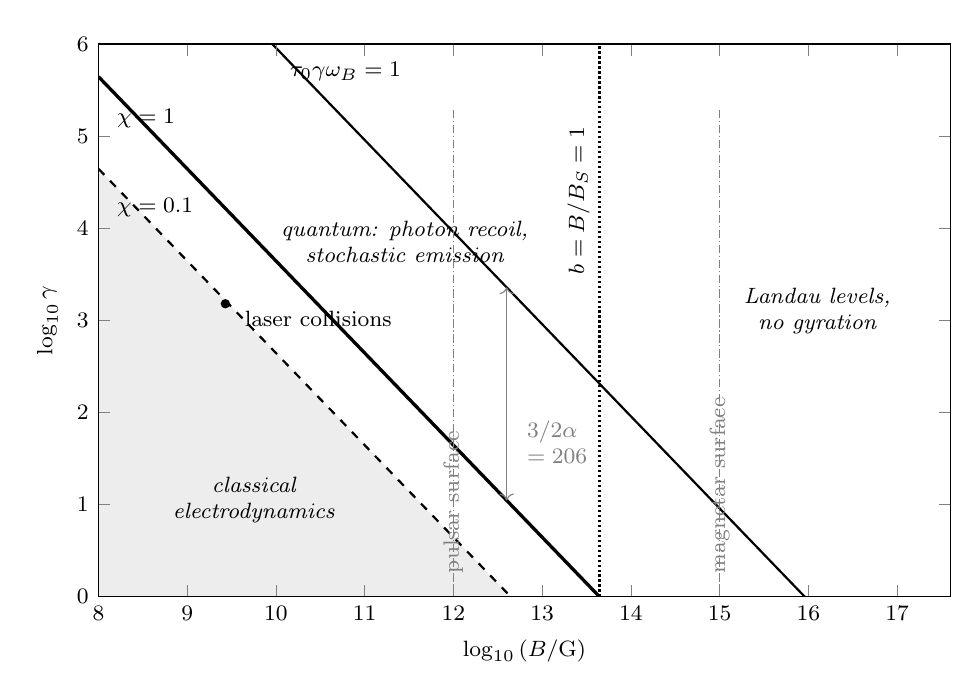
\begin{tikzpicture}
\begin{axis}[
  width=12.4cm, height=8.6cm,
  xlabel={$\log_{10}\,(B/\mathrm{G})$},
  ylabel={$\log_{10}\gamma$},
  xmin=8, xmax=17.6, ymin=0, ymax=6,
  xtick={8,9,10,11,12,13,14,15,16,17},
  ytick={0,1,2,3,4,5,6},
  axis on top, clip=true, samples=2, font=\footnotesize,
  legend style={draw=none,fill=none},
]

  %% ---- the classical wedge: below chi = 0.1 and left of B = B_S ----
  \fill[gray!14]
    (axis cs:8,0) -- (axis cs:8,4.645) -- (axis cs:12.645,0) -- cycle;

  %% ---- Landau quantization: B = B_S, vertical ----
  \addplot[thick,densely dotted,domain=0:6] coordinates {(13.645,0) (13.645,6)};
  \node[rotate=90,anchor=south,font=\footnotesize]
       at (axis cs:13.645,4.30) {$b=B/B_S=1$};

  %% ---- chi = 1 and chi = 0.1 ----
  \addplot[very thick,domain=8:17] {13.645 - x};
  \node[anchor=west,font=\footnotesize] at (axis cs:8.10,5.19) {$\chi=1$};

  \addplot[thick,dashed,domain=8:17] {12.645 - x};
  \node[anchor=west,font=\footnotesize] at (axis cs:8.10,4.22) {$\chi=0.1$};

  %% ---- classical radiation reaction becomes non-perturbative ----
  \addplot[thick,domain=8:17] {15.958 - x};
  \node[anchor=west,font=\footnotesize] at (axis cs:10.05,5.70)
       {$\taunought\gamma\omega_B=1$};

  %% ---- the gap between those two parallel lines, drawn where both are in view
  %%      at x = 12.6 they sit at y = 1.045 and y = 3.358 ----
  \draw[<->,gray] (axis cs:12.6,1.045) -- (axis cs:12.6,3.358);
  \node[anchor=west,font=\footnotesize,gray,align=left]
       at (axis cs:12.72,1.68) {$3/2\alpha$\\$=206$};

  %% ---- regime labels ----
  \node[font=\footnotesize\itshape,align=center] at (axis cs:9.75,1.05)
       {classical\\electrodynamics};
  \node[font=\footnotesize\itshape,align=center] at (axis cs:11.45,3.85)
       {quantum: photon recoil,\\stochastic emission};
  \node[font=\footnotesize\itshape,align=center] at (axis cs:16.1,3.1)
       {Landau levels,\\no gyration};

  %% ---- where things sit ----
  \fill (axis cs:9.43,3.18) circle (1.7pt);
  \node[anchor=west,font=\footnotesize] at (axis cs:9.54,3.02)
       {laser collisions};
  \draw[gray,densely dashdotted] (axis cs:12,0) -- (axis cs:12,5.3);
  \node[rotate=90,anchor=west,font=\footnotesize,gray]
       at (axis cs:12,0.15) {pulsar surface};
  \draw[gray,densely dashdotted] (axis cs:15,0) -- (axis cs:15,5.3);
  \node[rotate=90,anchor=west,font=\footnotesize,gray]
       at (axis cs:15,0.15) {magnetar surface};

\end{axis}
\end{tikzpicture}
\caption{Where classical electrodynamics applies. Shaded is the region in which
it does: $\chi\lesssim0.1$ and $B\lesssim B_S$. Crossing \emph{upward or to the
right} across any boundary leaves it, and the three boundaries fail in
different ways. Above $\chi=1$ a single photon carries a sizeable part of the
particle's energy, so the emission is quantum and stochastic. To the right of
$B=B_S$ the transverse motion is Landau quantized and there is no gyration for
an equation of motion to describe. The line $\taunought\gamma\omega_B=1$ is
where classical radiation reaction would itself become non-perturbative, which
is the regime Secs.~\ref{sec:lorentz} to \ref{sec:eliezer} are about --- and it
lies a factor $3/2\alpha=206$ above the line where the classical description of
the emission has already failed, so it is never reached. Laser--electron
collisions sit at $\chi\approx0.09$ for $a_0=10$ at $800$\,nm against a
$\gamma=1500$ beam, the relevant field being the $2\gamma E$ seen head-on, just inside the classical region and close enough to the
boundary to test it. Pulsar and magnetar surface fields are marked; at a
magnetar surface even a mildly relativistic electron is already past both
quantum boundaries.
\label{fig:regime}}
\end{figure}
.
%% Needs pgfplots, loaded in the main preamble.
%%
%% The (B, gamma) plane in log-log. Every boundary below is a computed number,
%% not a drawn one; the arithmetic is in the appendix of REVIEW_2026.md and
%% reproduced here:
%%
%%   B_S   = m^2 c^3 / (e hbar) = 4.414e13 G      log10 = 13.645
%%   B_cl  = m^2 c^4 / e^3      = 6.049e15 G      log10 = 15.782  ( = B_S/alpha )
%%   gamma B at tau_0 gamma omega_B = 1 : 3 m^2 c^4 / (2 e^3) = 9.073e15 G
%%                                                   log10 = 15.958
%%
%% Lines of constant gamma*B are straight with slope -1 here:
%%   chi = 0.1        log10 gamma = 12.645 - log10 B
%%   chi = 1          log10 gamma = 13.645 - log10 B
%%   tau_0 g w_B = 1  log10 gamma = 15.958 - log10 B
%% The last two are separated by a factor 3/(2 alpha) = 205.6, i.e. 2.31 decades.
%%
%% Laser point: a0 = 10 at 800 nm gives a lab field 1.34e9 G; head-on the
%% electron sees 2E = 2.68e9 G (log10 = 9.428), so with gamma = 1500
%% (log10 = 3.176) this is chi = 2 gamma E / B_S = 0.091.

\begin{figure}[htb]
\centering
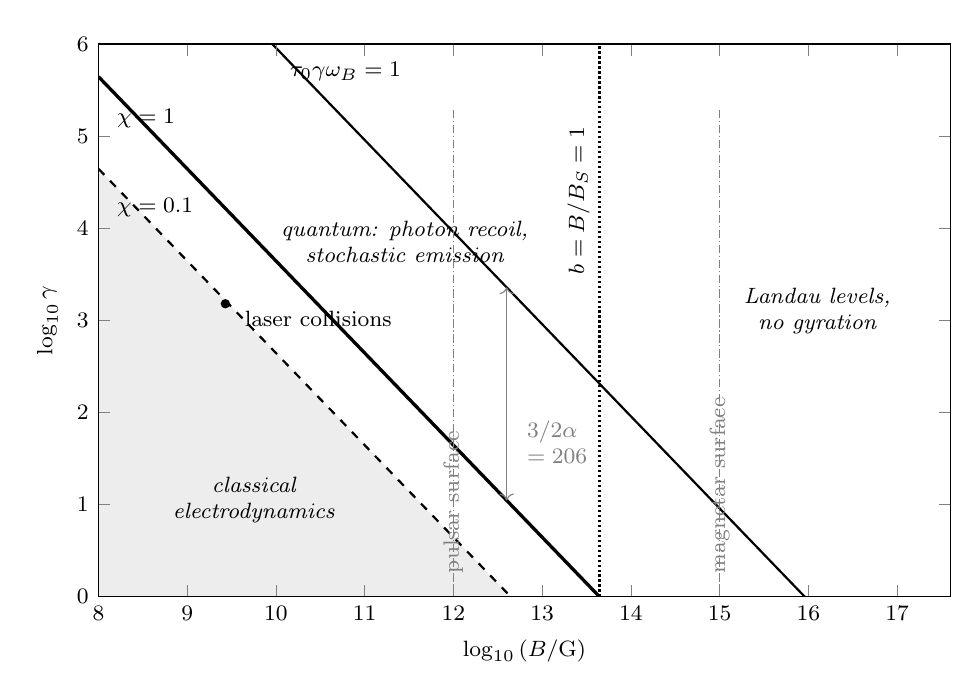
\begin{tikzpicture}
\begin{axis}[
  width=12.4cm, height=8.6cm,
  xlabel={$\log_{10}\,(B/\mathrm{G})$},
  ylabel={$\log_{10}\gamma$},
  xmin=8, xmax=17.6, ymin=0, ymax=6,
  xtick={8,9,10,11,12,13,14,15,16,17},
  ytick={0,1,2,3,4,5,6},
  axis on top, clip=true, samples=2, font=\footnotesize,
  legend style={draw=none,fill=none},
]

  %% ---- the classical wedge: below chi = 0.1 and left of B = B_S ----
  \fill[gray!14]
    (axis cs:8,0) -- (axis cs:8,4.645) -- (axis cs:12.645,0) -- cycle;

  %% ---- Landau quantization: B = B_S, vertical ----
  \addplot[thick,densely dotted,domain=0:6] coordinates {(13.645,0) (13.645,6)};
  \node[rotate=90,anchor=south,font=\footnotesize]
       at (axis cs:13.645,4.30) {$b=B/B_S=1$};

  %% ---- chi = 1 and chi = 0.1 ----
  \addplot[very thick,domain=8:17] {13.645 - x};
  \node[anchor=west,font=\footnotesize] at (axis cs:8.10,5.19) {$\chi=1$};

  \addplot[thick,dashed,domain=8:17] {12.645 - x};
  \node[anchor=west,font=\footnotesize] at (axis cs:8.10,4.22) {$\chi=0.1$};

  %% ---- classical radiation reaction becomes non-perturbative ----
  \addplot[thick,domain=8:17] {15.958 - x};
  \node[anchor=west,font=\footnotesize] at (axis cs:10.05,5.70)
       {$\taunought\gamma\omega_B=1$};

  %% ---- the gap between those two parallel lines, drawn where both are in view
  %%      at x = 12.6 they sit at y = 1.045 and y = 3.358 ----
  \draw[<->,gray] (axis cs:12.6,1.045) -- (axis cs:12.6,3.358);
  \node[anchor=west,font=\footnotesize,gray,align=left]
       at (axis cs:12.72,1.68) {$3/2\alpha$\\$=206$};

  %% ---- regime labels ----
  \node[font=\footnotesize\itshape,align=center] at (axis cs:9.75,1.05)
       {classical\\electrodynamics};
  \node[font=\footnotesize\itshape,align=center] at (axis cs:11.45,3.85)
       {quantum: photon recoil,\\stochastic emission};
  \node[font=\footnotesize\itshape,align=center] at (axis cs:16.1,3.1)
       {Landau levels,\\no gyration};

  %% ---- where things sit ----
  \fill (axis cs:9.43,3.18) circle (1.7pt);
  \node[anchor=west,font=\footnotesize] at (axis cs:9.54,3.02)
       {laser collisions};
  \draw[gray,densely dashdotted] (axis cs:12,0) -- (axis cs:12,5.3);
  \node[rotate=90,anchor=west,font=\footnotesize,gray]
       at (axis cs:12,0.15) {pulsar surface};
  \draw[gray,densely dashdotted] (axis cs:15,0) -- (axis cs:15,5.3);
  \node[rotate=90,anchor=west,font=\footnotesize,gray]
       at (axis cs:15,0.15) {magnetar surface};

\end{axis}
\end{tikzpicture}
\caption{Where classical electrodynamics applies. Shaded is the region in which
it does: $\chi\lesssim0.1$ and $B\lesssim B_S$. Crossing \emph{upward or to the
right} across any boundary leaves it, and the three boundaries fail in
different ways. Above $\chi=1$ a single photon carries a sizeable part of the
particle's energy, so the emission is quantum and stochastic. To the right of
$B=B_S$ the transverse motion is Landau quantized and there is no gyration for
an equation of motion to describe. The line $\taunought\gamma\omega_B=1$ is
where classical radiation reaction would itself become non-perturbative, which
is the regime Secs.~\ref{sec:lorentz} to \ref{sec:eliezer} are about --- and it
lies a factor $3/2\alpha=206$ above the line where the classical description of
the emission has already failed, so it is never reached. Laser--electron
collisions sit at $\chi\approx0.09$ for $a_0=10$ at $800$\,nm against a
$\gamma=1500$ beam, the relevant field being the $2\gamma E$ seen head-on, just inside the classical region and close enough to the
boundary to test it. Pulsar and magnetar surface fields are marked; at a
magnetar surface even a mildly relativistic electron is already past both
quantum boundaries.
\label{fig:regime}}
\end{figure}
.
%% Needs pgfplots, loaded in the main preamble.
%%
%% The (B, gamma) plane in log-log. Every boundary below is a computed number,
%% not a drawn one; the arithmetic is in the appendix of REVIEW_2026.md and
%% reproduced here:
%%
%%   B_S   = m^2 c^3 / (e hbar) = 4.414e13 G      log10 = 13.645
%%   B_cl  = m^2 c^4 / e^3      = 6.049e15 G      log10 = 15.782  ( = B_S/alpha )
%%   gamma B at tau_0 gamma omega_B = 1 : 3 m^2 c^4 / (2 e^3) = 9.073e15 G
%%                                                   log10 = 15.958
%%
%% Lines of constant gamma*B are straight with slope -1 here:
%%   chi = 0.1        log10 gamma = 12.645 - log10 B
%%   chi = 1          log10 gamma = 13.645 - log10 B
%%   tau_0 g w_B = 1  log10 gamma = 15.958 - log10 B
%% The last two are separated by a factor 3/(2 alpha) = 205.6, i.e. 2.31 decades.
%%
%% Laser point: a0 = 10 at 800 nm gives a lab field 1.34e9 G; head-on the
%% electron sees 2E = 2.68e9 G (log10 = 9.428), so with gamma = 1500
%% (log10 = 3.176) this is chi = 2 gamma E / B_S = 0.091.

\begin{figure}[htb]
\centering
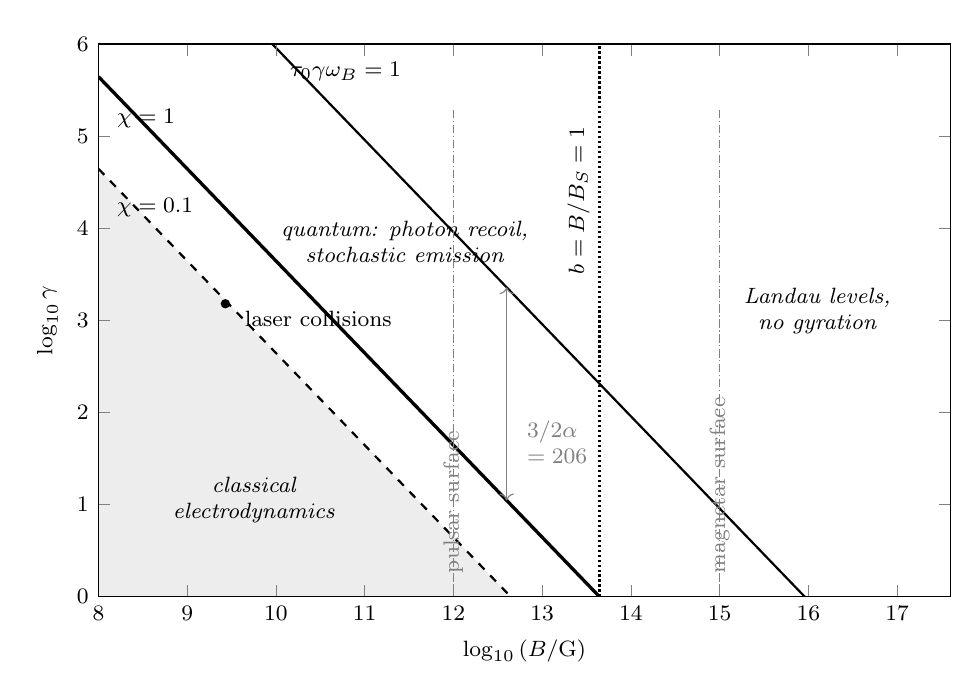
\begin{tikzpicture}
\begin{axis}[
  width=12.4cm, height=8.6cm,
  xlabel={$\log_{10}\,(B/\mathrm{G})$},
  ylabel={$\log_{10}\gamma$},
  xmin=8, xmax=17.6, ymin=0, ymax=6,
  xtick={8,9,10,11,12,13,14,15,16,17},
  ytick={0,1,2,3,4,5,6},
  axis on top, clip=true, samples=2, font=\footnotesize,
  legend style={draw=none,fill=none},
]

  %% ---- the classical wedge: below chi = 0.1 and left of B = B_S ----
  \fill[gray!14]
    (axis cs:8,0) -- (axis cs:8,4.645) -- (axis cs:12.645,0) -- cycle;

  %% ---- Landau quantization: B = B_S, vertical ----
  \addplot[thick,densely dotted,domain=0:6] coordinates {(13.645,0) (13.645,6)};
  \node[rotate=90,anchor=south,font=\footnotesize]
       at (axis cs:13.645,4.30) {$b=B/B_S=1$};

  %% ---- chi = 1 and chi = 0.1 ----
  \addplot[very thick,domain=8:17] {13.645 - x};
  \node[anchor=west,font=\footnotesize] at (axis cs:8.10,5.19) {$\chi=1$};

  \addplot[thick,dashed,domain=8:17] {12.645 - x};
  \node[anchor=west,font=\footnotesize] at (axis cs:8.10,4.22) {$\chi=0.1$};

  %% ---- classical radiation reaction becomes non-perturbative ----
  \addplot[thick,domain=8:17] {15.958 - x};
  \node[anchor=west,font=\footnotesize] at (axis cs:10.05,5.70)
       {$\taunought\gamma\omega_B=1$};

  %% ---- the gap between those two parallel lines, drawn where both are in view
  %%      at x = 12.6 they sit at y = 1.045 and y = 3.358 ----
  \draw[<->,gray] (axis cs:12.6,1.045) -- (axis cs:12.6,3.358);
  \node[anchor=west,font=\footnotesize,gray,align=left]
       at (axis cs:12.72,1.68) {$3/2\alpha$\\$=206$};

  %% ---- regime labels ----
  \node[font=\footnotesize\itshape,align=center] at (axis cs:9.75,1.05)
       {classical\\electrodynamics};
  \node[font=\footnotesize\itshape,align=center] at (axis cs:11.45,3.85)
       {quantum: photon recoil,\\stochastic emission};
  \node[font=\footnotesize\itshape,align=center] at (axis cs:16.1,3.1)
       {Landau levels,\\no gyration};

  %% ---- where things sit ----
  \fill (axis cs:9.43,3.18) circle (1.7pt);
  \node[anchor=west,font=\footnotesize] at (axis cs:9.54,3.02)
       {laser collisions};
  \draw[gray,densely dashdotted] (axis cs:12,0) -- (axis cs:12,5.3);
  \node[rotate=90,anchor=west,font=\footnotesize,gray]
       at (axis cs:12,0.15) {pulsar surface};
  \draw[gray,densely dashdotted] (axis cs:15,0) -- (axis cs:15,5.3);
  \node[rotate=90,anchor=west,font=\footnotesize,gray]
       at (axis cs:15,0.15) {magnetar surface};

\end{axis}
\end{tikzpicture}
\caption{Where classical electrodynamics applies. Shaded is the region in which
it does: $\chi\lesssim0.1$ and $B\lesssim B_S$. Crossing \emph{upward or to the
right} across any boundary leaves it, and the three boundaries fail in
different ways. Above $\chi=1$ a single photon carries a sizeable part of the
particle's energy, so the emission is quantum and stochastic. To the right of
$B=B_S$ the transverse motion is Landau quantized and there is no gyration for
an equation of motion to describe. The line $\taunought\gamma\omega_B=1$ is
where classical radiation reaction would itself become non-perturbative, which
is the regime Secs.~\ref{sec:lorentz} to \ref{sec:eliezer} are about --- and it
lies a factor $3/2\alpha=206$ above the line where the classical description of
the emission has already failed, so it is never reached. Laser--electron
collisions sit at $\chi\approx0.09$ for $a_0=10$ at $800$\,nm against a
$\gamma=1500$ beam, the relevant field being the $2\gamma E$ seen head-on, just inside the classical region and close enough to the
boundary to test it. Pulsar and magnetar surface fields are marked; at a
magnetar surface even a mildly relativistic electron is already past both
quantum boundaries.
\label{fig:regime}}
\end{figure}


Figure~\ref{fig:regime} puts the three boundaries in the $(B,\gamma)$ plane.
The classical region is the shaded wedge at the bottom left, and one leaves it
by going up or to the right.

The third row of the table is the one Secs.~\ref{sec:lorentz} to
\ref{sec:eliezer} were about. It is also the last of the three to arrive, and the ordering is not an
accident of numbers:
\begin{equation}
\frac{B_{\rm cl}}{B_S}
= \frac{m^2c^4/e^3}{m^2c^3/e\hbar}
= \frac{\hbar c}{e^2}
= \frac{1}{\alpha} \approx 137 .
\label{eq:ratio}
\end{equation}
The same statement can be made without reference to fields at all. The
classical electron radius and the reduced Compton wavelength stand in the ratio
\begin{equation}
\frac{r_0}{\lambda_C} = \frac{e^2/mc^2}{\hbar/mc} = \alpha ,
\label{eq:radii}
\end{equation}
so the length at which classical electrodynamics runs into itself lies inside
the length at which quantum mechanics has already taken over, and it lies
inside by exactly $\alpha$. Equation~(\ref{eq:ratio}) is Eq.~(\ref{eq:radii})
in the language of fields.

The consequence is worth stating flatly, because it settles the motivation of
everything before this section. The runaway of Sec.~\ref{sec:freesol}, the
pre-acceleration of Sec.~\ref{sec:asymptotic}, the merging of $\taunought$ with
the physical timescale --- these become $O(1)$ effects only at
$B_{\rm cl}$, and $B_{\rm cl}$ is $137$ times past the point where the
classical description of the emission has already failed. \emph{The classical
theory does not get to break down.} It is superseded well before its own
pathologies become measurable, which is why no experiment has ever seen a
runaway and why none ever will.

Where classical electrodynamics is still the right tool is correspondingly
specific: $\chi\lesssim0.1$. Three places qualify. Laser--electron collision
experiments work deliberately at $\chi\sim0.1$ to $1$, which is the transition
region and the only place the strength of the radiation reaction can be
measured against a classical prediction. The outer regions of pulsar
magnetospheres, far from the surface, have $B$ low enough for classical
treatment, and that is where the Aristotelian electrodynamics of
Sec.~\ref{sec:branchA} lives. And the classical result remains the $\chi\to0$
limit that any strong-field QED calculation has to reproduce, which is how such
calculations are checked.

None of this says that classical radiation reaction is wrong.
Section~\ref{sec:LLeq} stands and Eq.~(\ref{eq:LL}) is exact in its domain;
what the domain excludes is the regime in which the classical theory's own
difficulties would have become visible. Nor does it say the strong-field
problem is uninteresting. It says the problem there is a different one, and it
is worth setting down what that problem is, because it is where the subject
went.

Past $\chi\sim1$ the classical emission formula is replaced rather than
corrected. The radiated power becomes
\begin{equation}
P = g(\chi)\,P_{\rm cl},
\qquad
g(\chi)\simeq 0.56\,\chi^{-4/3} \quad (\chi\gg1),
\label{eq:gaunt}
\end{equation}
with $g$ the quantum suppression factor, and at $\chi=1$ the true power is
already about half the classical value. That much could be absorbed into an
equation of motion by rescaling a coefficient, and it is tempting to read it as
the measurement of $\zeta$ that Sec.~\ref{sec:lk-summary} asked for. It is not,
and the reason is the second change, which no rescaling reproduces.

Emission is not continuous. The electron radiates one photon at a time, and
once a single photon carries an appreciable fraction of the energy, two
electrons prepared identically do not follow the same trajectory: the energy
loss is a random variable and the final state is a distribution. This is
straggling, and it is not a correction to a deterministic law but a
statement that the law is the wrong kind of object. \emph{No equation of
motion, of any order, with any coefficient, produces a spread from identical
initial data.} Sections~\ref{sec:lk} and \ref{sec:eliezer} argued about which
ordinary differential equation to write down; past $\chi\sim1$ the answer is
none of them.

What is used instead is a kinetic description: photon emission sampled
event by event from the strong-field QED rates, usually under the
locally-constant-field approximation, with the particle pushed classically
between emissions; or a Fokker--Planck treatment when the second moment
suffices; or Eq.~(\ref{eq:gaunt}) inserted into Eq.~(\ref{eq:LL}) when only the
mean matters and the spread does not. The locally-constant-field approximation
is itself the subject of current work, since it is known to fail for the
low-energy part of the emitted spectrum.

\subsection{What has actually been measured}
\label{sec:experiment}

Sections~\ref{sec:lk} and \ref{sec:eliezer} argued on the only grounds
available to them, whether the solutions of a proposed equation look physical.
That is not the only ground available, and it is worth setting out what has
been measured, because the experimental record is both older and broader than
the recent laser work suggests, and most of it sits in the classical region of
Fig.~\ref{fig:regime} rather than outside it.

Each subsection below is one experiment or one class of them, in order of
increasing $\chi$, and each ends with the figure in the primary paper that
carries the result, so that the claim can be checked rather than taken on
trust. Table~\ref{tab:experiments} collects the same information.

\subsubsection{Storage rings have been measuring the coefficient for seventy
years}
\label{sec:rings}

Every electron storage ring is a radiation-reaction experiment that runs
continuously, and the quantity it measures is the coefficient of
Eq.~(\ref{eq:LL}) and nothing else. On a circular orbit of radius $\rho$ the
Larmor formula integrates over one turn to an energy loss
\begin{equation}
U_0 \;=\; \frac{4\pi}{3}\,\frac{e^2\gamma^4}{\rho},
\label{eq:U0}
\end{equation}
which is $\tfrac23 e^2\dot v^2/c^3$ carried around the ring, so the number in
front of it is the same $\taunought$ that Secs.~\ref{sec:lorentz} to
\ref{sec:eliezer} have been arguing about. That loss is what damps the betatron
and synchrotron oscillations, with damping times
\begin{equation}
\tau_i \;=\; \frac{2E_0T_0}{J_i\,U_0},
\qquad
J_x+J_y+J_s \;=\; 4,
\label{eq:robinson}
\end{equation}
$T_0$ being the revolution period and $J_i$ the partition numbers. The sum rule
is Robinson's theorem \citep{robinson1958}: the damping can be moved between the
three degrees of freedom by changing the lattice, but the total is fixed by the
radiated power alone. Both parts of Eq.~(\ref{eq:robinson}) are measured in
every machine that is commissioned. For a $3$~GeV ring with $\rho\sim10$~m the
loss is $\sim0.7$~MeV per turn and the damping time a few milliseconds, some
thousands of turns, which is short enough that a ring that did not damp would
not store beam at all.

The regime is deeply classical: $\gamma\approx6\times10^3$ in a $B=10^4$~G
bending field gives $\chi\approx1.3\times10^{-6}$, at the far lower left of
Fig.~\ref{fig:regime}. That is exactly why the result is worth stating, because
it settles a question the theoretical literature sometimes leaves open.
\emph{Radiation reaction is not a conjectural effect}, and a measured damping
time is a measurement of $\taunought$ on a real beam. The disputes of
Secs.~\ref{sec:LDdisc} to \ref{sec:eliezer} are disputes about what to do
with a term whose size was settled experimentally before any of them began.

\emph{Where to look.} There is no single canonical paper or figure here, which
is itself the point: it is accelerator engineering, not a result. The standard
derivation of Eqs.~(\ref{eq:U0}) and (\ref{eq:robinson}) is
\citet{sands1970}; the theorem is \citet{robinson1958}.

\subsubsection{The same machines have measured the granularity of the emission
since the 1970s}
\label{sec:excitation}

Those rings also measure the quantity Sec.~\ref{sec:classquantum} called the
signature of the quantum regime. Emission is by photons, so the energy loss
fluctuates, and the equilibrium energy spread is set by the balance of that
fluctuation against the damping of Eq.~(\ref{eq:robinson}):
\begin{equation}
\Big(\frac{\sigma_E}{E}\Big)^{\!2} \;=\; \frac{C_q\,\gamma^2}{J_s\,\rho},
\qquad
C_q \;=\; \frac{55}{32\sqrt3}\,\frac{\hbar}{mc}
\;=\; 3.83\times10^{-13}~\mathrm{m}.
\label{eq:cq}
\end{equation}
The constant is proportional to $\hbar$ and to nothing else, so a beam with a
measured energy spread is a measurement of the granularity: were the emission
continuous, $\sigma_E$ would be zero. The same shot noise sets the horizontal
emittance, and the spin polarizes radiatively by the Sokolov--Ternov effect
\citep{sokolov_ternov1964} to an asymptotic $8/5\sqrt3=92.4\%$, first seen at
ACO and VEPP-2 around 1971.

The consequence for Sec.~\ref{sec:classquantum} is that stochastic emission is
not a strong-field novelty. It has been observed for half a century at
$\chi\sim10^{-6}$, where it is a small diffusion superposed on a deterministic
drift and where Eq.~(\ref{eq:cq}) describes it completely. What changes at
$\chi\sim1$ is not that the emission becomes stochastic --- it always was ---
but that the diffusion stops being small compared with the drift, so that the
spread can no longer be carried as a correction to a deterministic trajectory.

\emph{Where to look.} \citet{sands1970} again for Eq.~(\ref{eq:cq}); the
figure worth reproducing is a polarization build-up curve from any of the
$e^+e^-$ rings, which shows the exponential approach to $92.4\%$ on the
Sokolov--Ternov time scale.

\subsubsection{A single trapped electron shows the effect is not collective,
and that it depends on the boundary}
\label{sec:penning}

A beam is many particles, and one could ask whether the damping is a collective
effect. It is not. The cyclotron motion of one electron in a Penning trap damps
radiatively at
\begin{equation}
\gamma_{\rm damp} \;=\; \taunought\,\omega_c^2,
\qquad
\omega_c=\frac{eB}{mc},
\label{eq:cyclodamp}
\end{equation}
which is the Abraham--Lorentz damping rate of Eq.~(\ref{eq:AL}) evaluated on a
circular orbit and nothing more; it is the rate for the amplitude, so the
cyclotron energy decays at $2\taunought\omega_c^2$. At $B=5$~T,
$\omega_c/2\pi=140$~GHz and Eq.~(\ref{eq:cyclodamp}) gives an energy lifetime
of about $0.1$~s, long enough to watch directly. It is measured on one particle, which is as clean a test of the
coefficient as exists.

The interesting part is that the measured rate is not always the free-space
one. \citet{gabrielse1985} found the decay inhibited by more than an order of
magnitude when the cyclotron frequency was tuned away from a mode of the
microwave cavity formed by the trap electrodes. This is the first observation
of inhibited spontaneous emission, and it makes a point that matters for these
notes: the self-force is not a property of the particle. It is a property of
the particle together with the field it radiates into, and changing the
boundary conditions on that field changes it. Nothing in
Secs.~\ref{sec:LDderiv} to \ref{sec:eliezer} could have anticipated this, because
all of them work in unbounded Minkowski space.

\emph{Where to look.} \citet{gabrielse1985}, the figure giving the measured
cyclotron decay rate as the trap is tuned through the cavity resonances; the
suppression is read off directly against the free-space value of
Eq.~(\ref{eq:cyclodamp}).

\subsubsection{E-144 did in 1997 the experiment the thesis said could not be
done}
\label{sec:e144}

The first strong-field experiment predates \citet{zhang2006} by nearly a decade.
At the SLAC Final Focus Test Beam a $46.6$~GeV electron beam was collided with
terawatt pulses of $527$~nm light at $\sim10^{18}$~W/cm$^2$, giving $\eta=0.36$
in the notation of Eq.~(\ref{eq:a0chi}) --- their $\eta$ is $a_0$ --- and
$\Upsilon=0.84\,\eta=0.3$, their $\Upsilon$ being $\chi$. Two results came out
of it. \citet{bula1996} observed nonlinear Compton scattering, an electron
absorbing several laser photons in one event. \citet{burke1997} then observed
electron--positron pairs from the collision of the backscattered GeV photon
with several more laser photons, $106\pm14$ positrons above background, and
this was the first observation of inelastic light-by-light scattering with real
photons only. The yield scaled as
\begin{equation}
R_{e^+} \;\propto\; \eta^{2n},
\qquad
n = 5.1\pm0.2\,(\mathrm{stat})\,^{+0.5}_{-0.8}\,(\mathrm{syst}),
\label{eq:e144}
\end{equation}
the fifth power of the intensity, which is the multiphoton threshold made
visible: the process needs at least five photons and the rate reports that
number back.

This is not a radiation-reaction measurement --- the electrons emitted at most
a few photons, so nothing recoiled appreciably --- but it establishes that
$\chi\sim0.3$ was experimentally accessible in 1997, and it is the direct
counterexample to the conclusion of Sec.~5 of \citet{zhang2006} that this
regime was out of reach.

\emph{Where to look.} \citet{burke1997}, Fig.~4: positron yield per laser shot
against $\eta$ on log axes, with the power-law fit of Eq.~(\ref{eq:e144}) and
the shaded $95\%$ background limit. Fig.~3 of the same paper is the raw
laser-on minus laser-off positron spectrum.

\subsubsection{Aligned crystals reach $\chi\sim1$ with no laser at all}
\label{sec:crystal}

A crystal aligned to a beam presents a channelled particle with the coherent
field of an atomic string, of order $10^{11}$~V/cm, and in the rest frame of a
$100$~GeV particle that is already comparable with $B_S$.
\citet{wistisen2018} sent $178.2$~GeV positrons along the $\langle111\rangle$
axis of silicon crystals $3.8$ and $10.0$~mm thick, reaching $\chi\lesssim1.4$,
and measured the emitted photon spectrum. In that regime each positron emits
several photons carrying an appreciable fraction of its own energy, so the
recoil is not a perturbation and the spectrum is sensitive to how it is
treated. They compared four calculations --- classical with radiation reaction,
semiclassical, quantum with radiation reaction, and quantum without --- and only
the quantum treatment including recoil reproduced the data.

The platform matters because its systematics have nothing in common with a
laser collision. The field is static in the lab, the target is a solid with a
known thickness, and the number of interacting particles is not in doubt; there
is no beam overlap to estimate, which is the dominant uncertainty in everything
in Sec.~\ref{sec:laser2018}. An agreement between crystal and laser data is
therefore a stronger statement than either alone.

\emph{Where to look.} \citet{wistisen2018}, Fig.~3: background-subtracted
photon power spectrum for the two thicknesses, panels (a) and (b), with the
four model curves overlaid. Fig.~4 of the same paper shows the four models on
their own, without the detector response folded in, which is the cleaner figure
for seeing how far apart the classical and quantum predictions actually are.

\subsubsection{The 2018 laser collisions saw radiation reaction but could not
separate the models}
\label{sec:laser2018}

The modern line begins with two experiments on the same laser in the same year.
The controlled quantities are
\begin{equation}
a_0 = \frac{eE}{mc\omega},
\qquad
\chi = \frac{2\gamma a_0\hbar\omega}{mc^2},
\label{eq:a0chi}
\end{equation}
the factor $2\gamma$ being the boost of the laser field into the electron rest
frame in a head-on collision; $a_0=10$ at $800$~nm against a $\gamma=1500$ beam
gives $\chi\approx0.09$, the point marked in Fig.~\ref{fig:regime}.

\citet{cole2018} collided a laser-wakefield beam above $500$~MeV with a pulse
at $a_0>10$ and measured two things at once: the electron energy after the
collision and the critical energy of the $\gamma$-ray spectrum, above $30$~MeV.
Neither alone is conclusive, because $a_0$ is not known shot to shot, but the
\emph{correlation} between them is, since each model of radiation reaction
predicts a different curve in the $(\varepsilon_{\rm final},
\varepsilon_{\rm crit})$ plane parameterised by $a_0$ along its length. The
data preferred a quantum description. \citet{poder2018} pushed to beams above
$2$~GeV at $4\times10^{20}$~W/cm$^2$, where the electrons see about a quarter
of the critical field, and lost up to $30\%$ of their energy; comparing against
four models --- Lorentz force only, Landau--Lifshitz, semiclassical, and full
QED --- the classical Landau--Lifshitz curve overshot the loss and the two
quantum treatments did not.

Neither experiment separated the quantum treatments from one another, and
neither was a high-significance exclusion of the classical one. The reason was
the same in both: the dominant uncertainty is the spatial and temporal overlap
of two beams a few microns across, which is not a statistical error and does
not improve with more shots.

\emph{Where to look.} \citet{cole2018}, Fig.~9 of arXiv:1707.06821:
$\varepsilon_{\rm crit}$ against $\varepsilon_{\rm final}$, four data points,
with shaded bands showing what each model would produce for $a_0$ uniform on
$[4,20]$ --- the bands overlap, which is the honest picture of the
discrimination available in 2018. \citet{poder2018}, Fig.~4 of
arXiv:1709.01861: the measured post-collision electron spectrum against the
four models in panels (a)--(d), which is the single most legible
model-comparison figure in this literature.

\subsubsection{The 2026 measurement separates the models, and the classical one
loses}
\label{sec:los2026}

The discrimination that 2018 could not make has now been made.
\citet{los2026} report the first observation of strong-field radiation reaction
at above $5\sigma$ in which quantum effects matter, using a $609$~MeV beam
against a pulse of peak $a_0=21.4\pm1.8$, with $a_0$ between $7$ and $13$
inferred for the shots analysed. The method is what the 2018 work lacked:
over $600$ collisions and $608$ null shots, so that the difference between hit
and null distributions can be established statistically, followed by a Bayesian
inference on the ten highest-yield shots that treats the unknown $a_0$ as a
parameter to be marginalised rather than a systematic to be quoted. The result
is a Bayes factor favouring the quantum-continuous and quantum-stochastic
models over the classical one, driven by the classical model predicting too
much energy loss. The two quantum models are still not separated from each
other.

The parameter to note is $\chi$: at most $0.13$ at focus and $0.05$ to $0.1$
for the shots used. That is not deep in the quantum regime; it is the
$\chi=0.1$ line of Fig.~\ref{fig:regime}. The classical description of the
emission fails, measurably and at high significance, exactly where that figure
says it should, and this is the strongest evidence available that the boundary
drawn there is the physical one.

\emph{Where to look.} \citet{los2026}, arXiv:2407.12071. Fig.~4: the measured
post-collision electron spectrum for the highest-yield shot against the three
models. Fig.~5: the Bayes factors, shot by shot and combined, which is the
figure that carries the $5\sigma$ claim and the one to reproduce if only one is
wanted.

\subsubsection{LUXE and E-320 are being built to scan $\chi$ through unity}
\label{sec:future}

Everything above either sits well below $\chi=1$ or, in the crystal case,
reaches it in a target that cannot be tuned. Two experiments now under
construction are designed to sweep through it. LUXE at DESY will collide the
$16.5$~GeV European XFEL beam with a laser, and E-320 at SLAC will do the same
with the $10$~GeV FACET-II beam; both can vary the laser intensity at fixed
beam energy, so that $\chi$ becomes a knob rather than a shot-to-shot accident.
That is what is needed to test $g(\chi)$ of Eq.~(\ref{eq:gaunt}) as a function
rather than at a point, and to reach the regime where the locally-constant-field
approximation of Sec.~\ref{sec:classquantum} can be checked against data.

\begin{deluxetable}{llccl}
\tablecaption{The experimental record, in order of increasing $\chi$.
\label{tab:experiments}}
\tablehead{
\colhead{Experiment} & \colhead{When} & \colhead{$\chi$} &
\colhead{Measured} & \colhead{Fig.}
}
\startdata
Penning trap        & 1985     & $10^{-9}$     & cyclotron damping, one electron & ---            \\
Storage rings       & 1950s--  & $10^{-6}$     & damping times, Robinson rule    & ---            \\
Quantum excitation  & 1970s--  & $10^{-6}$     & energy spread, polarization     & ---            \\
E-144               & 1996--97 & $0.3$         & Compton, pair creation          & 4              \\
Cole 2018           & 2018     & $\sim0.1$     & $\varepsilon_{\rm crit}$ vs.\ $\varepsilon_{\rm final}$ & 9$^{\rm a}$ \\
Poder 2018          & 2018     & $\sim0.25$    & electron spectrum               & 4$^{\rm a}$    \\
Wistisen 2018       & 2018     & $\lesssim1.4$ & photon spectrum                 & 3              \\
Los 2026            & 2026     & $0.05$--$0.1$ & Bayes factors, $>5\sigma$       & 4, 5$^{\rm a}$ \\
LUXE, E-320         & building & through $1$   & $g(\chi)$ as a function         & ---            \\
\enddata
\tablecomments{Full references in the text, Secs.~\ref{sec:rings} to
\ref{sec:future}. $^{\rm a}$Figure numbers of the preprint version, which is the
version checked here. The first three rows are standing accelerator practice
rather than single experiments and have no canonical figure.}
\end{deluxetable}

\medskip

Three things follow from the list. The first is that the existence of radiation
reaction, and the accuracy of its classical description where that description
applies, are not open questions and have not been for seventy years; the rings
of Sec.~\ref{sec:rings} settle it, on beams and, in Sec.~\ref{sec:penning}, on
one particle at a time. The second is that the strong-field regime was reached
in 1997, not in 2018, and the 2006 assessment of what was feasible was already
nine years out of date when it was written. The third is that the classical
description has now been excluded, at $5\sigma$ and at $\chi\approx0.1$, which
is the first time any of the equations in these notes has been ruled out by
data rather than by argument --- and what was ruled out was
Eq.~(\ref{eq:LL}), the survivor of Secs.~\ref{sec:lorentz} to
\ref{sec:eliezer}, in the one place where it was ever going to fail.

\subsection{Open questions, and one that nobody has attempted}
\label{sec:stillopen}
A list of open questions is only worth reading if the list of settled ones is
given first, since otherwise every unanswered question looks equally live. So:
Eq.~(\ref{eq:LD}) is an effective equation and not a fundamental one, and
reduction of order is its physical content, not a numerical convenience
(Sec.~\ref{sec:verdict}). The $B^\mu$ freedom is a field redefinition in the
point-particle limit (Sec.~\ref{sec:LLeq}). A derivation exists that needs no
world-tube and no undetermined four-vector \citep{gralla2009}. The singular
part of the field exerts no force \citep{detweiler_whiting2003}. And
Eq.~(\ref{eq:LL}) is the standard classical workhorse, for the reasons of
Sec.~\ref{sec:whyLL}. This is the standard reading in 2026.

\subsubsection{Every physical open question is now on the quantum side}
\label{sec:openquantum}

What remains is a short list, and its most striking feature is where all of it
sits. Not one physical item is a question about the classical equation of
motion.

\emph{Which description holds in the transition region.} At $\chi\sim0.1$ to
$1$ the candidates are the quantum-continuous treatment, in which the mean
radiated power is suppressed by $g(\chi)$ of Eq.~(\ref{eq:gaunt}) and the motion
stays deterministic, and stochastic emission, in which identical initial data
give a distribution of final states. \citet{los2026} excluded the classical
alternative but could not separate these two, because they predict the same mean
and differ only in the spread, which the incoming beam's own energy spread
masks. This is the live question, and it is a question about which \emph{kinetic}
description is right, not which equation of motion is.

\emph{The rates themselves.} The locally-constant-field approximation
underlying every calculation in the previous paragraph is known to fail for the
low-energy end of the emitted spectrum, and $g(\chi)$ at $\chi\gg1$ is not
tested at all. LUXE and E-320 (Sec.~\ref{sec:future}) are built to address
exactly this.

\emph{Whether an equation of motion returns.} Above $\chi\sim1$ a deterministic
single trajectory is no longer the right object, and the description is a
kinetic equation for a distribution. Whether anything recognisable as an
equation of motion survives that limit, for the mean or for a suitably defined
effective particle, is open. It is the closest thing in the modern subject to
the question Secs.~\ref{sec:lorentz} to \ref{sec:eliezer} were asking.

\subsubsection{The one classical question left is mathematical, not physical}
\label{sec:openclassical}

The $\taunought$ expansion of Eq.~(\ref{eq:slowmanifold}) is asymptotic, not
convergent, and its resummation and Borel structure have been studied without
being settled. This is a real question and it should be listed, but its status
should be stated honestly: Eq.~(\ref{eq:formgap}) bounds the whole expansion
beyond first order by $2.4\times10^{-5}$ anywhere the classical description
applies at all. Nothing observable depends on the answer. The same estimate
disposes of the Landau--Lifshitz versus Ford--O'Connell disagreement, which is
sometimes written as though it were open: it is open, and it is unmeasurable,
and those are compatible.

\subsubsection{What nobody has attempted: how well is the coefficient known?}
\label{sec:unattempted}

The remaining item is of a different kind, and it is flagged as such because it
is not on the field's agenda. It is the proposal of \citet{zhang2026}, and it is
listed here as a gap these notes claim to have found rather than as a question
the literature is asking.

Section~\ref{sec:whycoefficient} argued that $\zeta$ of Eq.~(\ref{eq:zetadef})
is the only number in this subject to which an experiment is linearly
sensitive. The question is then embarrassingly simple: \emph{what is the
experimental bound on $\zeta$?} There does not appear to be a published answer.

The reason there is none is visible in Sec.~\ref{sec:experiment}, and it is a
gap between two communities rather than a hard problem. Storage-ring damping
data are directly sensitive to $\zeta$, at $\chi\sim10^{-6}$ where $g(\chi)$
differs from unity by one part in $10^{5}$. But to accelerator physics a
damping time is a machine parameter, not a test of electrodynamics. These notes
have not found a standard bound quoted in this language. The strong-field
experiments of Secs.~\ref{sec:e144} to \ref{sec:los2026} do treat their
measurements as tests of electrodynamics, but they test the \emph{form}: three
or four precomputed model curves, and the question of which fits. Every one of
them holds
$\zeta=1$ fixed while doing so, because no reason to do otherwise has ever been
offered.

Two things follow, and they are worth separating because they differ in
difficulty and in interest.

The first is bookkeeping: convert existing classical-regime data into an
interval for $\zeta$. The expected answer is $\zeta=1$, and the result is a
number with an error bar rather than a discovery. It is nonetheless a number
that a subject eighty years old ought to be able to quote and cannot.

The second is not bookkeeping. In the transition region the observable is
$P_{\rm rad} = \zeta\,g(\chi)\,P_{\rm cl}$, in which $\zeta$ and the quantum
suppression enter multiplicatively. Every strong-field result quoted in
Sec.~\ref{sec:experiment} is a statement about $g$ obtained by holding $\zeta$
fixed. Whether those conclusions survive letting both float has not been
examined. The model selection of \citet{los2026} may be partly absorbing a
coefficient. It may also be that the two are cleanly separable, in which case
the answer is a joint constraint on a pair rather than a ranking of three
models. Or they may be degenerate, in which case a headline result rests on an
assumption nobody stated. Either outcome is worth knowing, and neither requires
new data.

The honest scoping is the one \citet{zhang2026} gives. This is not a programme
to reopen the classical theory of the electron, and it should not be written as
one. The classical theory is settled for the purposes of these notes, as
Secs.~\ref{sec:verdict} to \ref{sec:whichequation} argued at length. It is a
narrow question about the
observability of, and the existing constraints on, one coefficient. The risks
are stated there too, and the sharpest is the obvious one: $\zeta$ may
decohere against collision geometry and beam-parameter systematics badly enough
that no useful interval comes out. That is a result as well, and a cheaper one
to obtain than to speculate about.

\subsection{What survives is the coefficient, not the equation}
\label{sec:survives}
\note{Settle the naming debt here, moved out of Sec.~\ref{sec:verdict}, since it
is a statement about what survived: comparing Eq.~(\ref{eq:LL1d}) with
Eq.~(\ref{eq:third}), both start from Eq.~(\ref{eq:LD}), one replaces $\ddot q$
by a derivative of the force and lowers the order, the other adds $\dddot q$ and
raises it, and the two carry the same name --- the first being the
Eliezer--Ford--O'Connell equation \citep{eliezer1948,ford_oconnell1991}, free of
runaways and a live experimental candidate.
The upward branch of Sec.~\ref{sec:eliezer} does not survive, and it runs
opposite to the cure: each retained order adds an unphysical mode rather than
removing the one already there. The sideways branch of Sec.~\ref{sec:lk} does.
Strip the scaffolding and what is left, Eq.~(\ref{eq:zeta}), is a number that
data can constrain, and the transition region of Sec.~\ref{sec:LLeq} is where
it can be constrained. And the Aristotle motion of Sec.~\ref{sec:branchA}
survives under another name, as the Aristotelian electrodynamics now used in
pulsar magnetosphere modelling, where the field fixes the velocity rather than
the acceleration. Close on the shape of the whole thing: the pathology these
notes tracked for five sections turns out to be an artefact of treating an
effective equation as a fundamental one, while the parameter invented to cure
it is the only part that can be measured.}

%% ===================================================================
%% MATERIAL DEFERRED TO A LATER ROUND (not part of this outline):
%%   - Sec. 4 of the 2006 text: general-relativistic corrections,
%%     the "effective metric" ansatz, the iterated Einstein solution.
%%   - Sec. 5 of the 2006 text: the discriminating experiment,
%%     dP/dOmega as the observable, and the feasibility estimate.
%%   - Part 2 of the 2006 text: the MiSaTaQuWa equation.
%%   - The twenty-years-on commentary: order reduction (LL, EFO),
%%     the slow-manifold theorem, Gralla-Harte-Wald, and the
%%     2018-2026 laser-electron collision experiments.
%%
%%     A draft of this existed briefly as a subsection 3.7, "What to do
%%     instead", and was removed: placed there it announced the answer
%%     before Secs. 4 and 5 had been argued, and pre-judged Sec. 5 in so
%%     many words. Its content, to be written up after Sec. 5:
%%       * (LD) is an effective equation, not a literal third-order law;
%%         tau_0 is the warning label and the bad solution lives on
%%         exactly that timescale.
%%       * Reduction of order: differentiate ma = F_ext, substitute for
%%         adot in the reaction term, keep first order in tau_0. Gives
%%         Landau-Lifshitz: second order, no runaway, no pre-acceleration,
%%         and agrees with LD to the order a classical point-particle
%%         equation can be trusted at.
%%       * The geometric version: the physical solutions of LD lie on a
%%         slow manifold; Spohn (2000) makes this precise for the
%%         Abraham-Lorentz model, and LL is its first-order description.
%%         Gralla-Harte-Wald (2009) put the self-force on a firmer footing
%%         without treating the bare LD initial-value problem as
%%         fundamental.
%%       * The verdict on the two routes of Secs. 4 and 5: changing the
%%         coefficient survives as a phenomenological test of radiation
%%         reaction; raising the order runs opposite to the modern cure
%%         and should be expected to add unphysical modes rather than
%%         remove the one already there.
%% ===================================================================

%% Works the sections still to be written will need. Delete this command if the
%% reference list should carry only what is actually cited so far.
\nocite{eliezer1947,eliezer1948,ford_oconnell1991,spohn2000,gralla2009,
dewitt_brehme1960,hobbs1968,detweiler_whiting2003,mino_sasaki_tanaka1997,
quinn_wald1997,weinberg1972,cole2018,poder2018,poisson1999}

\bibliography{notes}
\bibliographystyle{aasjournalv7}

\end{document}
